%_____________________________________________________________________________
%=============================================================================
% main.tex v10 (02-10-2016) \ldots dibuat oleh Lionov - Informatika FTIS UNPAR 
% 
% Ini adalah file utama (main.tex), berisi perintah-perintah yang khusus 
% dibuat untuk template ini
%
% 			JANGAN MENGUBAH APAPUN DI DALAM FILE INI, 
%			KECUALI ANDA TAHU APA YANG ANDA LAKUKAN !!! 
% 
% Perubahan pada versi 10 (02-10-2016):
%	- Perubahan nama file dari main.tex menjadi skripsi.tex
%	- Perubahan style bibliography dari "ieeetr" menjadi "compj" yang digunakan
%     di jurnal "The Computer Journal" yg diterbitkan oleh Oxford University 
%     Press/British Computer Society
%	- Penempatan gambar otomatis di folder "Gambar", jadi tidak perlu menuliskan
%	  nama folder lagi (\includegraphics{Gambar/tes} --> \includegraphics{tes})
%	- Perubahan font menjadi latin modern yg sdh banyak digunakan di jurnal2 intl
%   - Perbaikan kecil: jeda antara ttd pembimbing dan penguji
%	- Pembimbing Tunggal --> Pembimbing (karena sdh jelas tunggal 
%	- Penggunaan kantlipsum (output bhs inggris) sebagai pengganti lipsum
%	- \onespacing otomatis untuk buku skripsi final, untuk buku sidang tetap 
%	  \onehalfspacing
%	- Perbaikan hfill dan hfil yang masih menjadi masalah, bagian itu dipindahkan
%	  ke dekat deklarasi Daftar Isi
%_____________________________________________________________________________
%=============================================================================

%setup.tex
\documentclass[11pt,a4paper,twoside,openright,notitlepage]{report}  

\usepackage{lmodern} %font latin modern 
\usepackage[bahasa]{babel} %bahasa indonesia
\usepackage[T1]{fontenc}  %encoding
% \usepackage{mathptmx}
% \usepackage{venturisold}
% \usepackage{helvet}
% \usepackage{fouriernc} 
\usepackage{abstract} %manipulasi abstract
\usepackage{chappg} % format daftar isi 
\usepackage{color} %warna 
\usepackage{etoolbox} %untuk programming if-then
\usepackage{fancyhdr} %format header & footer
\usepackage{float} %penempatan gambar di tempat yg seharusnya 
\usepackage[inner=2.5cm,outer=2cm,top=2.5cm,bottom=2.5cm]{geometry} %margin
\usepackage{graphicx} %gambar
\usepackage{listings} %source code
\usepackage{lscape} %landscape untuk source code
\usepackage{multicol} %multiple column
\usepackage{ifthen} % if then
\usepackage[pagewise]{lineno} %line numbering
\usepackage{kantlipsum} % untuk dummy text
\usepackage{titlesec} %judul header
\usepackage{tocbibind} %daftar isi, gambar, tabel dll
\usepackage{tocloft} % format daftar isi 
\usepackage{setspace} %line spacing
\usepackage{xstring} %manipulasi string
\usepackage[plainpages=false,pdfpagelabels,unicode]{hyperref} %\autoref, \phantomsection & link 
\usepackage{emptypage} %halaman kosong antar bab
\graphicspath{{./Gambar/}} 

\usepackage{lcg}
\newcommand{\random}{\rand\arabic{rand}}

\let\abstractname\Abstrak

\normalfont
\DeclareFontShape{T1}{lmr}{bx}{sc} { <-> ssub * cmr/bx/sc }{}

\titleformat{\chapter}[display] {\Large\bfseries\centering}{\MakeUppercase{\chaptertitlename} \thechapter}{15pt}{\Large\MakeUppercase}

\renewcommand{\cftchapfont}{\scshape \bfseries}

% Tidak perlu ada kata "Bab", "Gambar" atau "Tabel" di daftar 
% \renewcommand{\cftchappresnum}{{\bf \scshape Bab} } 
% \renewcommand{\cftchapnumwidth}{1.5cm}
% \renewcommand{\cftfigpresnum}{{Gambar\ }} 
% \renewcommand{\cftfignumwidth}{2.5cm}
% \renewcommand{\cfttabpresnum}{{Tabel\ }} 
% \renewcommand{\cfttabnumwidth}{2cm}


\newcommand{\vnama}{Jane Doe}
\newcommand{\vlnama}{John Doe}
\newcommand{\vnpm}{1992700001}
\newcommand{\vprodiINA}{SAINS}
\newcommand{\vprodiENG}{SCIENCE}
\newcommand{\vstaINA}{UJIAN}
\newcommand{\vstaENG}{EXAM}
%\newcommand{\vjudul}{Judul Skripsi/Tugas Akhir}
\newcommand{\vpembu}{Plato}
\newcommand{\vpembs}{Euclid}
\newcommand{\vpengi}{Plato}
\newcommand{\vpengii}{Euclid}
\newcommand{\vtanggal}{1}
\newcommand{\vbulan}{Januari}
\newcommand{\vtahun}{1970}
\newcommand{\vmode}{final}
\newcommand{\vspacing}{double}
\newcommand{\vlineno}{yes}
\newcommand{\vkunciina}{Skripsi, Tugas Akhir}
\newcommand{\vkuncieng}{Undergraduate Thesis, Final Project}
\newcommand{\vkajur}{Jack Doe}
\newcommand{\vkajurmat}{Jack Doe}
\newcommand{\vkajurfis}{Jack Doe}
\newcommand{\vkajurtif}{Jack Doe}
\newcommand{\vtabel}{}
\newcommand{\vgambar}{}
\newcommand{\vdierror}{}

\newcommand{\namanpm}[2]{
	\renewcommand{\vstaINA}{<<SKRIPSI/TUGAS AKHIR>>}
	\renewcommand{\vprodiINA}{<<MATEMATIKA/FISIKA/TEKNIK INFORMATIKA>>}
	\renewcommand{\vstaENG}{<<FINAL PROJECT/UNDERGRADUATE THESIS>>}
	\renewcommand{\vprodiENG}{<<MATHEMATICS/PHYSICS/INFORMATICS>>}
	\renewcommand{\vnama}{\uppercase{#1}} \renewcommand{\vlnama}{#1} \hypersetup{pdfauthor={#2 - #1}}
	\renewcommand{\vnpm}{#2} \hypersetup{pdfcreator={#2}} \StrChar{\vnpm}{6}[\vprodiN]
%	\renewcommand{\vnpm}{#2} \hypersetup{pdfcreator={\jobname}} \StrChar{\vnpm}{6}[\vprodiN]
	\ifdefstring{\vprodiN}{1}{
		\renewcommand{\vprodiINA}{MATEMATIKA} \renewcommand{\vprodiENG}{MATHEMATICS} 
		\renewcommand{\vstaINA}{SKRIPSI} \renewcommand{\vstaENG}{FINAL PROJECT} \renewcommand{\vkajur}{\vkajurmat}}{}
	\ifdefstring{\vprodiN}{2}{
		\renewcommand{\vprodiINA}{FISIKA} \renewcommand{\vprodiENG}{PHYSICS} 
		\renewcommand{\vstaINA}{TUGAS AKHIR} \renewcommand{\vstaENG}{FINAL PROJECT} \renewcommand{\vkajur}{\vkajurfis}}{}
	\ifdefstring{\vprodiN}{3}{
		\renewcommand{\vprodiINA}{TEKNIK INFORMATIKA} \renewcommand{\vprodiENG}{INFORMATICS} 
		\renewcommand{\vstaINA}{SKRIPSI} \renewcommand{\vstaENG}{UNDERGRADUATE THESIS} \renewcommand{\vkajur}{\vkajurtif}}{}
	}

%\newcommand{\judul}[1]{\renewcommand{\vjudul}{\uppercase{#1}}\hypersetup{pdftitle={#1}, pdfsubject={#1}}}
\newcommand{\pembimbing}[2]{\renewcommand{\vpembu}{#1}\renewcommand{\vpembs}{#2}}
\newcommand{\penguji}[2]{\renewcommand{\vpengi}{#1}\renewcommand{\vpengii}{#2}}
\newcommand{\kajur}[3]{\renewcommand{\vkajurmat}{#1}\renewcommand{\vkajurfis}{#2}\renewcommand{\vkajurtif}{#3}}
\renewcommand{\vbulan}{<<bulan>>}
\newcommand{\tanggal}[3]{\renewcommand{\vtanggal}{#1}\renewcommand{\vtahun}{#3}
	\newcommand{\vcbulan}{#2}
	\ifdefstring{\vcbulan}{1}{\renewcommand{\vbulan}{Januari}}{}
	\ifdefstring{\vcbulan}{2}{\renewcommand{\vbulan}{Februari}}{}
	\ifdefstring{\vcbulan}{3}{\renewcommand{\vbulan}{Maret}}{}
	\ifdefstring{\vcbulan}{4}{\renewcommand{\vbulan}{April}}{}
	\ifdefstring{\vcbulan}{5}{\renewcommand{\vbulan}{Mei}}{}
	\ifdefstring{\vcbulan}{6}{\renewcommand{\vbulan}{Juni}}{}
	\ifdefstring{\vcbulan}{7}{\renewcommand{\vbulan}{Juli}}{}
	\ifdefstring{\vcbulan}{8}{\renewcommand{\vbulan}{Agustus}}{}
	\ifdefstring{\vcbulan}{9}{\renewcommand{\vbulan}{September}}{}
	\ifdefstring{\vcbulan}{10}{\renewcommand{\vbulan}{Oktober}}{}
	\ifdefstring{\vcbulan}{11}{\renewcommand{\vbulan}{November}}{}
	\ifdefstring{\vcbulan}{12}{\renewcommand{\vbulan}{Desember}}{}	
}

\newcommand{\judulINA}[1]{\newcommand{\vjudulINA}{\uppercase{#1}}\hypersetup{pdftitle={#1},pdfsubject={#1}}}
\newcommand{\judulENG}[1]{\newcommand{\vjudulENG}{\uppercase{#1}}\hypersetup{pdftitle={#1},pdfsubject={#1}}}
\newcommand{\abstrakINA}[1]{\newcommand{\vabstrakina}{#1}}
\newcommand{\abstrakENG}[1]{\newcommand{\vabstrakeng}{#1}}
\newcommand{\kunciINA}[1]{\renewcommand{\vkunciina}{#1} \hypersetup{pdfkeywords={#1}}}
\newcommand{\kunciENG}[1]{\renewcommand{\vkuncieng}{#1}}
\newcommand{\untuk}[1]{\newcommand{\vuntuk}{#1}}
\newcommand{\prakata}[1]{\newcommand{\vprakata}{#1}}
\newcommand{\mode}[1]{\renewcommand{\vmode}{#1}}
\newcommand{\linespacing}[1]{\renewcommand{\vspacing}{#1}}
\newcommand{\linenumber}[1]{\renewcommand{\vlineno}{#1}}

\newcommand{\daftarIsiError}[1]{\renewcommand{\vdierror}{#1}} 
\newcommand{\gambar}[1]{\renewcommand{\vgambar}{#1}}
\newcommand{\tabel}[1]{\renewcommand{\vtabel}{#1}}

\newcommand{\bab}[1]{\newcommand{\vbab}{#1}}
\newcommand{\lampiran}[1]{\renewcommand{\vlmp}{#1}} 

\newcommand{\vpilbab}{0}
\newcommand{\vbaba}{0}\newcommand{\vbabb}{0}\newcommand{\vbabc}{0}
\newcommand{\vbabd}{0}\newcommand{\vbabe}{0}\newcommand{\vbabf}{0}
\newcommand{\vbabg}{0}\newcommand{\vbabh}{0}\newcommand{\vbabi}{0}
\newcommand{\vpillmp}{0}
\newcommand{\vlmpa}{0}\newcommand{\vlmpb}{0}\newcommand{\vlmpc}{0}
\newcommand{\vlmpd}{0}\newcommand{\vlmpe}{0}\newcommand{\vlmpf}{0}
\newcommand{\vlmpg}{0}\newcommand{\vlmph}{0}\newcommand{\vlmpi}{0}
\newcommand{\vlmp}{x}

%	\ifdefempty{#1}{\bab{1,2,3,4,5,6,7,8,9} \tampilbab{\vbab}}{
\newcommand{\tampilbab}[1]{
	\ifdefempty{#1}{
		\renewcommand{\vbaba}{1}\renewcommand{\vbabb}{1}\renewcommand{\vbabc}{1}
		\renewcommand{\vbabd}{1}\renewcommand{\vbabe}{1}\renewcommand{\vbabf}{1}
		\renewcommand{\vbabg}{1}\renewcommand{\vbabh}{1}\renewcommand{\vbabi}{1}}{
	\renewcommand{\do}[1]{
		\renewcommand{\vpilbab}{##1}
		\ifdefstring{\vpilbab}{1}{\renewcommand{\vbaba}{1}}{}
		\ifdefstring{\vpilbab}{2}{\renewcommand{\vbabb}{1}}{}
		\ifdefstring{\vpilbab}{3}{\renewcommand{\vbabc}{1}}{}
		\ifdefstring{\vpilbab}{4}{\renewcommand{\vbabd}{1}}{}
		\ifdefstring{\vpilbab}{5}{\renewcommand{\vbabe}{1}}{}
		\ifdefstring{\vpilbab}{6}{\renewcommand{\vbabf}{1}}{}
		\ifdefstring{\vpilbab}{7}{\renewcommand{\vbabg}{1}}{}
		\ifdefstring{\vpilbab}{8}{\renewcommand{\vbabh}{1}}{}
		\ifdefstring{\vpilbab}{9}{\renewcommand{\vbabi}{1}}{}
	}
	\expandafter\docsvlist\expandafter{#1}
	}
}

\newcommand{\tampillmp}[1]{
	\ifdefempty{#1}{
		\renewcommand{\vlmpa}{1}\renewcommand{\vlmpb}{1}\renewcommand{\vlmpc}{1}
		\renewcommand{\vlmpd}{1}\renewcommand{\vlmpe}{1}\renewcommand{\vlmpf}{1}
		\renewcommand{\vlmpg}{1}\renewcommand{\vlmph}{1}\renewcommand{\vlmpi}{1}}{
	\ifdefstring{#1}{-1}{ }{
		\renewcommand{\do}[1]{ 
			\renewcommand{\vpillmp}{##1}
			\ifdefstring{\vpillmp}{A}{\renewcommand{\vlmpa}{1}}{}
			\ifdefstring{\vpillmp}{B}{\renewcommand{\vlmpb}{1}}{}
			\ifdefstring{\vpillmp}{C}{\renewcommand{\vlmpc}{1}}{}
			\ifdefstring{\vpillmp}{D}{\renewcommand{\vlmpd}{1}}{}
			\ifdefstring{\vpillmp}{E}{\renewcommand{\vlmpe}{1}}{}
			\ifdefstring{\vpillmp}{F}{\renewcommand{\vlmpf}{1}}{}
			\ifdefstring{\vpillmp}{G}{\renewcommand{\vlmpg}{1}}{}
			\ifdefstring{\vpillmp}{H}{\renewcommand{\vlmph}{1}}{}
			\ifdefstring{\vpillmp}{I}{\renewcommand{\vlmpi}{1}}{}}
		}
	\expandafter\docsvlist\expandafter{#1}
	}
}

\newcommand{\appspacing}{
	\ifdefstring{\vspacing}{single}{\singlespacing}{}
	\ifdefstring{\vspacing}{onehalf}{\onehalfspacing}{}
	\ifdefstring{\vspacing}{double}{\doublespacing}{}
	\ifdefstring{\vmode}{sidang}{\onehalfspacing}{}	
	\ifdefstring{\vmode}{sidang_akhir}{\onehalfspacing}{}	
	\ifdefstring{\vmode}{final}{\singlespacing}{}
}

\newcommand{\appline}{
	\ifdefstring{\vmode}{final}{\renewcommand{\vlineno}{no}}{}
	\ifdefstring{\vlineno}{yes}{\linenumbers \def\linenumberfont{\normalfont\tiny\sffamily}}{}
	\ifdefstring{\vlineno}{no}{\lstset{numbers=left, stepnumber=1, numbersep=5pt}}{}
	
}

\newcommand{\appmargin}{
	\ifdefstring{\vmode}{final}{}{\newgeometry{inner=3cm,outer=2.75cm,top=2cm,bottom=2cm}}
}

\renewcommand{\abstractnamefont}{\bf \MakeUppercase}

\makeatletter
\def\headrule{{%
  \if@fancyplain\let\headrulewidth\plainheadrulewidth\fi
  \hrule\@height\footrulewidth\@width\headwidth\vskip2pt%
  \hrule\@height\headrulewidth\@width\headwidth\vskip-\headrulewidth\vskip-4pt
}}
\def\footrule{}

\def\cleardoublepage{
	\clearpage
	\if@twoside \ifodd\c@page
	\else
		\hbox{}
		\vspace{\fill} 
		\thispagestyle{empty}
		\newpage
	\if@twocolumn\hbox{}\newpage\fi\fi\fi}
\makeatother

\renewcommand{\headrulewidth}{1.25pt}
\renewcommand{\footrulewidth}{0.25pt}

\setlength{\headheight}{15pt}
\fancyhead[LE,RO]{\thepage}
\fancyhead[RE]{\small{\textsc{\nouppercase{\leftmark}}}}
\fancyhead[LO]{\small{\textsc{\nouppercase{\rightmark}}}}
\fancyfoot{}

\hypersetup{unicode=true,colorlinks=true,linkcolor=blue,citecolor=green,filecolor=magenta, urlcolor=cyan}

\lstset{basicstyle=\tiny, commentstyle=\color{blue}}
\lstset{frame=leftline, tabsize=4, breaklines=true}

%end setup.tex

%_____________________________________________________________________________
%=============================================================================
% data.tex v7 (30-11-2015) \ldots dibuat oleh Lionov - Informatika FTIS UNPAR
%
% Perubahan pada versi 7 (30-11-2015)
%	- Perubahan nomor bagian karena penyisipan Bagian V
%	- Penambahan Bagian V : pengaturan kemunculan daftar gambar dan/atau tabel 
%	  dipindahkan dari main.tex
%	- Penambahan Bagian XV : tempat untuk menambahkan perintah yang dibuat 
%	  sendiri, dipindahkan dari main.tex
%	- Penambahan Bagian 0 : perintah bagi yang caption daftar isi tidak bisa
%	  ke bagian tengah
%
% Perubahan pada versi sebelumnya dapat dilihat di bagian akhir file ini
%_____________________________________________________________________________
%=============================================================================

%=============================================================================
% 								PETUNJUK
%=============================================================================
% Ini adalah file data (data.tex)
% Masukkan ke dalam file ini, data-data yang diperlukan oleh template ini
% Cara memasukkan data dijelaskan di setiap bagian
% Data yang WAJIB dan HARUS diisi dengan baik dan benar adalah SELURUHNYA !!
% Hilangkan tanda << dan >> jika anda menemukannya
%=============================================================================

%_____________________________________________________________________________
%=============================================================================
% 								BAGIAN 0
%=============================================================================
% PERHATIAN!! PERHATIAN!! Bagian ini hanya ada untuk sementara saja
% Jika "DAFTAR ISI" tidak bisa berada di bagian tengah halaman, isi dengan XXX
% jika sudah benar posisinya, biarkan kosong (i.e. \daftarIsiError{ })
%=============================================================================
\daftarIsiError{ }
%=============================================================================

%_____________________________________________________________________________
%=============================================================================
% 								BAGIAN I
%=============================================================================
% Tambahkan package2 lain yang anda butuhkan di sini
%=============================================================================
\usepackage{booktabs} 
\usepackage[table]{xcolor}
\usepackage{longtable}
\usepackage{amsmath}
\usepackage{todo}
%=============================================================================

%_____________________________________________________________________________
%=============================================================================
% 								BAGIAN II
%=============================================================================
% Mode dokumen: menetukan halaman depan dari dokumen, apakah harus mengandung 
% prakata/pernyataan/abstrak dll (termasuk daftar gambar/tabel/isi) ?
% - kosong : tidak ada halaman depan sama sekali (untuk dokumen yang 
%            dipergunakan pada proses bimbingan)
% - cover : cover saja tanpa daftar isi, gambar dan tabel
% - sidang : cover, daftar isi, gambar, tabel (IT: UTS-UAS Seminar 
%			 dan UTS TA)
% - sidang_akhir : mode sidang + abstrak + abstract
% - final : seluruh halaman awal dokumen (untuk cetak final)
% Jika tidak ingin mencetak daftar tabel/gambar (misalkan karena tidak ada 
% isinya), edit manual di baris 439 dan 440 pada file main.tex
%=============================================================================
%\mode{kosong}
% \mode{cover}
% \mode{sidang}
%\mode{sidang_akhir}
\mode{final} 
%=============================================================================

%_____________________________________________________________________________
%=============================================================================
% 								BAGIAN III
%=============================================================================
% Line numbering: penomoran setiap baris, otomatis di-reset setiap berganti
% halaman
% - yes: setiap baris diberi nomor
% - no : baris tidak diberi nomor, otomatis untuk mode final
%=============================================================================
\linenumber{yes}
%=============================================================================

%_____________________________________________________________________________
%=============================================================================
% 								BAGIAN IV
%=============================================================================
% Linespacing: jarak antara baris 
% - single: opsi yang disediakan untuk bimbingan, jika pembimbing tidak
%            keberatan (untuk menghemat kertas)
% - onehalf: default dan wajib (dan otomatis) jika ingin mencetak dokumen
%            final/untuk sidang.
% - double : jarak yang lebih lebar lagi, jika pembimbing berniat memberi 
%            catatan yg banyak di antara baris (dianjurkan untuk bimbingan)
%=============================================================================
\linespacing{single}
%\linespacing{onehalf}
%\linespacing{double}
%=============================================================================

%_____________________________________________________________________________
%=============================================================================
% 								BAGIAN V
%=============================================================================
% Tidak semua skripsi memuat gambar dan/atau tabel. Untuk skripsi yang seperti
% itu, tidak diperlukan Daftar Gambar dan Daftar Tabel. Sayangnya hal ini 
% sulit dilakukan secara manual karena membutuhkan kedisiplinan pengguna 
% template.  
% Jika tidak akan menampilkan Daftar Gambar/Tabel, isi dengan NO. Jika ingin
% menampilkan, kosongkan parameter (i.e. \gambar{ }, \tabel{ })
%=============================================================================
\gambar{ }
\tabel{ }
%=============================================================================

%_____________________________________________________________________________
%=============================================================================
% 								BAGIAN VI
%=============================================================================
% Bab yang akan dicetak: isi dengan angka 1,2,3 s.d 9, sehingga bisa digunakan
% untuk mencetak hanya 1 atau beberapa bab saja
% Jika lebih dari 1 bab, pisahkan dengan ',', bab akan dicetak terurut sesuai 
% urutan bab (e.g. \bab{1,2,3}).
% Untuk mencetak seluruh bab, kosongkan parameter (i.e. \bab{ })  
% Catatan: Jika ingin menambahkan bab ke-10 dan seterusnya, harus dilakukan 
% secara manual
%=============================================================================
\bab{}
%=============================================================================

%_____________________________________________________________________________
%=============================================================================
% 								BAGIAN VII
%=============================================================================
% Lampiran yang akan dicetak: isi dengan huruf A,B,C s.d I, sehingga bisa 
% digunakan untuk mencetak hanya 1 atau beberapa lampiran saja
% Jika lebih dari 1 lampiran, pisahkan dengan ',', lampiran akan dicetak 
% terurut sesuai urutan lampiran (e.g. \bab{A,B,C}).
% Jika tidak ingin mencetak lampiran apapun, isi dengan -1 (i.e. \lampiran{-1})
% Untuk mencetak seluruh mapiran, kosongkan parameter (i.e. \lampiran{ })  
% Catatan: Jika ingin menambahkan lampiran ke-J dan seterusnya, harus 
% dilakukan secara manual
%=============================================================================
\lampiran{ }
%=============================================================================

%_____________________________________________________________________________
%=============================================================================
% 								BAGIAN VIII
%=============================================================================
% Data diri dan skripsi/tugas akhir
% - namanpm: Nama dan NPM anda, penggunaan huruf besar untuk nama harus benar
%			 dan gunakan 10 digit npm UNPAR, PASTIKAN BAHWA BENAR !!!
%			 (e.g. \namanpm{Jane Doe}{1992710001}
% - judul : Dalam bahasa Indonesia, perhatikan penggunaan huruf besar, judul
%			tidak menggunakan huruf besar seluruhnya !!! 
% - tanggal : isi dengan {tangga}{bulan}{tahun} dalam angka numerik, jangan 
%			  menuliskan kata (e.g. AGUSTUS) dalam isian bulan
%			  Tanggal ini adalah tanggal dimana anda akan melaksanakan sidang 
%			  ujian akhir skripsi/tugas akhir
% - pembimbing: isi dengan pembimbing anda, lihat daftar dosen di file dosen.tex
%				jika pembimbing hanya 1, kosongkan parameter kedua 
%				(e.g. \pembimbing{\JND}{  } ) , \JND adalah kode dosen
% - penguji : isi dengan para penguji anda, lihat daftar dosen di file dosen.tex
%				(e.g. \penguji{\JHD}{\JCD} ) , \JND dan \JCD adalah kode dosen
% !!Lihat singkatan pembimbing dan penguji anda di file dosen.tex
%=============================================================================
\namanpm{Dony Erlangga}{2012730071}	%hilangkan tanda << & >>
\tanggal{26}{09}{2016}			%hilangkan tanda << & >>
\pembimbing{\TAB}{} %hilangkan tanda << & >>    
\penguji{}{} 				%hilangkan tanda << & >>
%=============================================================================

%_____________________________________________________________________________
%=============================================================================
% 								BAGIAN IX
%=============================================================================
% Judul dan title : judul bhs indonesia dan inggris
% - judulINA: judul dalam bahasa indonesia
% - judulENG: title in english
% PERHATIAN: - langsung mulai setelah '{' awal, jangan mulai menulis di baris 
%			   bawahnya
%			 - Gunakan \texorpdfstring{\\}{} untuk pindah ke baris baru
%			 - Judul TIDAK ditulis dengan menggunakan huruf besar seluruhnya !!
%			 - Gunakan perintah \texorpdfstring{\\}{} untuk baris baru
%=============================================================================
\judulINA{SIKSA (Sistem Informasi Kebutuhan Surat Akademik)}
\judulENG{<<Judul Bahasa Inggris>>}
%_____________________________________________________________________________
%=============================================================================
% 								BAGIAN X
%=============================================================================
% Abstrak dan abstract : abstrak bhs indonesia dan inggris
% - abstrakINA: abstrak bahasa indonesia
% - abstrakENG: abstract in english
% PERHATIAN: langsung mulai setelah '{' awal, jangan mulai menulis di baris 
%			 bawahnya
%=============================================================================
\abstrakINA{<<Tuliskan abstrak anda di sini, dalam bahasa Indonesia>> \lipsum[5]}
\abstrakENG{<<Tuliskan abstrak anda di sini, dalam bahasa Inggris>> \lipsum[5]} 
%=============================================================================

%_____________________________________________________________________________
%=============================================================================
% 								BAGIAN XI
%=============================================================================
% Kata-kata kunci dan keywords : diletakkan di bawah abstrak (ina dan eng)
% - kunciINA: kata-kata kunci dalam bahasa indonesia
% - kunciENG: keywords in english
%=============================================================================
\kunciINA{<<Tuliskan di sini kata-kata kunci yang anda gunakan, dalam bahasa Indonesia>>}
\kunciENG{<<Tuliskan di sini kata-kata kunci yang anda gunakan, dalam bahasa Inggris>>}
%=============================================================================

%_____________________________________________________________________________
%=============================================================================
% 								BAGIAN XII
%=============================================================================
% Persembahan : kepada siapa anda mempersembahkan skripsi ini ...
%=============================================================================
\untuk{<<kepada siapa anda mempersembahkan skripsi ini\ldots?>>}
%=============================================================================

%_____________________________________________________________________________
%=============================================================================
% 								BAGIAN XIII
%=============================================================================
% Kata Pengantar: tempat anda menuliskan kata pengantar dan ucapan terima 
% kasih kepada yang telah membantu anda bla bla bla ....  
%=============================================================================
\prakata{\lipsum[3]}
%=============================================================================

%_____________________________________________________________________________
%=============================================================================
% 								BAGIAN XIV
%=============================================================================
% Tambahkan hyphen (pemenggalan kata) yang anda butuhkan di sini 
%=============================================================================
\hyphenation{ma-te-ma-ti-ka}
\hyphenation{fi-si-ka}
\hyphenation{tek-nik}
\hyphenation{in-for-ma-ti-ka}
%=============================================================================

%_____________________________________________________________________________
%=============================================================================
% 								BAGIAN XV
%=============================================================================
% Tambahkan perintah yang anda buat sendiri di sini 
%=============================================================================
\newcommand{\vtemplateauthor}{lionov}
%=============================================================================

%=============================================================================
% Perubahan pada versi 6 (13-04-2015)
% 	- Perubahan untuk data-data ``template" menjadi lebih generik dan 
%	  menggunakan tanda << dan >>
% Perubahan pada versi 5 (10-11-2013)
% 	- Perbaikan pada memasukkan bab : tidak perlu menuliskan apapun untuk 
%	  memasukkan seluruh bab (bagian V)
% 	- Perbaikan pada memasukkan lampiran : tidak perlu menuliskan apapun untuk
%	  memasukkan seluruh lampiran atau -1 jika tidak memasukkan apapun
% Perubahan pada versi 4 (21-10-2012)
%	- Data dosen dipindah ke dosen.tex agar jika ada perubahan/update data 
%	  dosen, mahasiswa tidak perlu mengubah data.tex
%	- Perubahan pada keterangan dosen	
% Perubahan pada versi 3 (06-08-2012)
% 	- Perubahan pada beberapa keterangan 
% Perubahan pada versi 2 (09-07-2012):
% 	- Menambahkan data judul dalam bahasa inggris
% 	- Membuat bagian khusus untuk judul (bagian VIII)
% 	- Perbaikan pada gelar dosen
% Versi 1 (08-11-2011)
%=============================================================================
%_____________________________________________________________________________
%=============================================================================
% dosen.tex v5 (30-11-2015) \ldots dibuat oleh Lionov - Informatika FTIS UNPAR
%
% Perubahan pada versi 5 (30-11-2015)
% 	- Perubahan ketua jurusan matematika menjadi JDL
% 	- Perubahan ketua jurusan teknik informatika menjadi MAR
%	- Penghapusan dosen (Hariman,Farica,Lukcy,Verli,Wahyu)
%	- Penambahan dosen (Risti, Bagoes, Reinard, Haryanto)
%	- Perbaikan gelar (Ferry, Rusli, Fla, Kian Ming, Wono, Gede, Pascal)
%	- Penggunaan thin-space untuk spasi pada nama, agar tidak terpotong
%
% Perubahan pada versi sebelumnya dapat dilihat di bagian akhir file ini
%_____________________________________________________________________________
%=============================================================================

%=============================================================================
% Data dosen dan kajur FTIS - JANGAN MENGUBAH APAPUN DI BAGIAN INI, KECUALI
% untuk mengubah kajur (jika kajur telah berganti orang) atau menambahkan 
% pembimbing anda yang tidak/belum tercantum pada daftar ini atau 
% memperbaiki penulisan gelar jika penguji anda meminta
% perintah: \kajur{1}{2}{3} 1: Matematika 2: Fisika 3: Teknik Informatika
%=============================================================================
% CATATAN UNTUK MAHASISWA TEKNIK INFORMATIKA :
% dosen yang ditandai * :
% - jika menjadi penguji,tetap,hapus komentar (tanda % dan *) agar dapat digunakan
% - jika menjadi pembimbing, harus diganti namanya dengan dosen lain, ikuti
% 	petunjuk dari koordinator Skripsi !
% - khusus untuk MAR, harus diganti juga sesuai petunjuk koordinator
%=============================================================================

\kajur{\JDL}{\PNG}{Mariskha\,Tri\,Adithia,\,P.D.Eng} 

%dummy person
\newcommand{\JND}{Jane\,Doe} 
\newcommand{\JHD}{John\,Doe}
\newcommand{\JCD}{Jack\,Doe}

% Dosen-dosen Program Studi Matematika
\newcommand{\JDL}{Dr.\,Julius\,Dharma\,Lesmono}
\newcommand{\FAR}{Farah\,Kristiani,\,M.Si.}
\newcommand{\ERW}{Erwinna\,Chendra,\,M.Si.}
\newcommand{\FJP}{Dr.\,Ferry\,Jaya\,Permana,\,ASAI}
\newcommand{\AGS}{Agus\,Sukmana,\,M.Sc.}
\newcommand{\WSB}{Prof.\,M.\,Wono\,Setya\,Budhi,\,Ph.D.}
\newcommand{\LIM}{Liem\,Chin,\,M.Si.}
\newcommand{\IWS}{Iwan\,Sugiarto,\,M.Si.}
\newcommand{\IVM}{Ivonne\,Martin,\,M.Sc.}
\newcommand{\OWN}{Livia\,Owen,\,M.Si.}
\newcommand{\BNY}{Benny\,Yong,\,M.Si.}
\newcommand{\TFK}{Taufik\,Limansyah,\,M.T.}
\newcommand{\MRA}{Maria\,Anestasia,\,M.Si.}

% Dosen-dosen Program Studi Fisika
\newcommand{\PCT}{Paulus\,Cahyono\,Tjiang,\,Ph.D.}
\newcommand{\BSB}{Prof.\,B.\,Suprapto\,Brotosiswojo,\,Ph.D.}
\newcommand{\RUS}{Aloysius\,Rusli,\,Ph.D.}
\newcommand{\KMG}{Kian\,Ming,\,M.Si.}
\newcommand{\SHS}{Sylvia\,Hastuti\,Sutanto,\,Ph.D.}
\newcommand{\JVS}{Janto\,Vincent\,Sulungbudi,\,S.Si.}
\newcommand{\FLA}{Flaviana,\,M.T.}
\newcommand{\PNG}{Philips\,Nicolas\,Gunawidjaja,\,Ph.D.}
\newcommand{\ELK}{Elok\,Fidiani,\,M.Sc.}
\newcommand{\RIS}{Risti\,Suryantari,\,M.Sc.}
\newcommand{\HAS}{Haryanto\,Siahaan,\,Ph.D.}
\newcommand{\RND}{Reinard\,Primulando,\,Ph.D.}

% Dosen-dosen Program Studi Teknik Informatika
\newcommand{\CEN}{Dr.rer.nat.\,Cecilia\,Esti\,Nugraheni}
\newcommand{\VSM}{Dr.\,Veronica\,Sri\,Moertini}
\newcommand{\RDL}{Rosa\,De\,Lima,\,M.Kom.}
\newcommand{\TAB}{Dott.\,Thomas\,Anung\,Basuki}
\newcommand{\LNV}{Lionov,\,M.Sc.}
% \newcommand{\OSS}{Dr.\,Oerip\,S.\,Santoso}
% * \newcommand{\MAR}{Mariskha\,Tri\,Adithia,\,P.D.Eng}
\newcommand{\LCA}{Luciana\,Abednego,\,M.T.}
\newcommand{\ELH}{Elisati\,Hulu,\,M.T.}
% * \newcommand{\CAN}{Chandra\,Wijaya,\,M.T.}
\newcommand{\GDK}{Gede\,Karya,\,M.T.,\,CISA}
\newcommand{\NIS}{Nico\,Saputro,\,M.T.}
% * \newcommand{\JNH}{Joanna\,Helga,\,M.Sc.}
% * \newcommand{\PAS}{Pascal\,Alfadian,\,M.Comp.} 
% * \newcommand{\HUS}{Husnul\,Hakim,\,M.T.} 
% * \newcommand{\VAN}{Vania\,Natali,\,M.T.} 
% * \newcommand{\BHR}{Aditya\,Bagoes\,Saputra,\,M.T.} 

%=============================================================================
% Perubahan pada versi 4 (01-03-2014)
% 	- Perubahan ketua jurusan teknik informatika menjadi TAB
%	- Penambahan dosen jurusan informatika (Lucky)
%
% Perubahan pada versi 3 (10-11-2013)
% 	- Perubahan ketua jurusan teknik informatika menjadi MAR
%	- Penambahan dosen jurusan informatika (Joanna, Wahyu)
%	- Penghapusan dosen informatika (Lucky, Dharu)
%
% Perubahan pada versi 2 (25-02-2013)
% 	- Tambahan catatan untuk mhs T. Inf. terkait dosen yg tidak bisa menjadi pemb.
% 	- Update data gelar untuk Taufik (MAT)
% 	- Penambahan baru (Farica-Fisika, Husnul-T.Informatika)
% 	- Dosen keluar atau tidak menjadi pembimbing lagi (Nisa, Ghifary)
%
% Versi 1 (21-10-2012)
% 	- Data dosen dipindah dari data.tex agar jika ada perubahan/update data dosen
%     mahasiswa tidak perlu mengubah data.tex
% 	- Beberapa dosen Informatika yang tidak boleh menjadi pembimbing digantikan OSS
% 	- Update data gelar untuk Maria (MAT)
% 	- Penambahan baru (Flaviana-Fisika, Elok-Fisika)
% 	- Dosen keluar atau tidak menjadi pembimbing lagi (Monika, David)
%=============================================================================

\begin{document}

\raggedbottom

\def\bibname{Daftar Referensi}
\def\abstractname{Abstrak}

\pagestyle{empty}

%depan.tex
\ifdefstring{\vmode}{kosong}{}{

\pagenumbering{roman}

%cover INA
\begin{center}
	{\Large\bf \vstaINA \\} 	\vspace{1.5cm}
	{\Large \bf \vjudulINA \\} \vspace{2.5cm}
	
\includegraphics[scale=0.4]{Gambar/logo-unpar}\\ \vspace{1cm}
	{\Large \bf \vnama \\} \vspace{0.5cm}
	{\Large \bf NPM: \vnpm \\}
	\vfill
	\Large{ \textbf { 
		PROGRAM STUDI \vprodiINA \\
		FAKULTAS TEKNOLOGI INFORMASI DAN SAINS\\
		UNIVERSITAS KATOLIK PARAHYANGAN\\
		\vtahun 
	}}
\end{center}
\cleardoublepage

%cover ENG
\begin{center}
	{\Large\bf \vstaENG \\} 	\vspace{1.5cm}
	{\Large \bf \vjudulENG \\} \vspace{2.5cm}
	
\includegraphics[scale=0.4]{Gambar/logo-unpar}\\ \vspace{1cm}
	{\Large \bf \vnama \\} \vspace{0.5cm}
	{\Large \bf NPM: \vnpm \\}
	\vfill
	\Large{ \textbf { 
		DEPARTMENT OF \vprodiENG \\
		FACULTY OF INFORMATION TECHNOLOGY AND SCIENCES\\
		PARAHYANGAN CATHOLIC UNIVERSITY\\
		\vtahun 
	}}
\end{center}
\cleardoublepage


% Lembar pengesahan
\ifdefstring{\vmode}{final}{
\begin{center}
	{\Large\bf LEMBAR PENGESAHAN \\} 	\vspace{1.5cm}
	{\Large \bf \vjudulINA \\} 			\vspace{1cm}
	{\Large \bf \vnama \\}				\vspace{0.5cm}
	{\Large \bf NPM: \vnpm \\}			\vspace{1.5cm}
	\large{ \bfseries{
		\begin{centering} 
			Bandung, \vtanggal\ \vbulan\ \vtahun \\ \vspace{0.25cm} Menyetujui,\\
			\vspace{0.75cm}
			\ifdefempty{\vpembs}
					{\centering Pembimbing\\ \vspace{2.25cm} \vpembu\\}
					{ 	\begin{minipage}[b]{0.46\linewidth}
							\centering Pembimbing Utama \\ \vspace{2.5cm} \vpembu \\
						\end{minipage} \hspace{0.5cm}
						\begin{minipage}[b]{0.46\linewidth}
							\centering Pembimbing Pendamping \\	\vspace{2.5cm} \vpembs \\
						\end{minipage}	
					}
		\end{centering} 
		\vspace{1.5cm}\\
		\begin{centering}	
			\begin{minipage}[b]{0.46\linewidth}
				\centering Ketua Tim Penguji \\ \vspace{2.5cm} \vpengi \\
			\end{minipage} \hspace{0.5cm}
			\begin{minipage}[b]{0.46\linewidth}
				\centering Anggota Tim Penguji \\ \vspace{2.5cm} \vpengii 
			\end{minipage}
		\end{centering}
		\vspace{1.5cm} \\
		\centering Mengetahui,\\ \vspace{0.5cm}	
		Ketua Program Studi \\ \vspace{2.5cm} \vkajur\\
	}}			
\end{center}
\cleardoublepage

% Lembar Pernyataan
\vspace*{4cm}
{\Large\bf \centering PERNYATAAN\\} \vspace{1cm}
\noindent
Dengan ini saya yang bertandatangan di bawah ini menyatakan bahwa \MakeLowercase{\vstaINA} dengan judul:  \vspace{0.5cm}
\begin{center}
	{\large \bf \vjudulINA \\}
\end{center}
\vspace{0.75cm}
adalah benar-benar karya saya sendiri, dan saya tidak melakukan penjiplakan atau pengutipan dengan cara-cara yang tidak sesuai dengan etika keilmuan yang berlaku dalam masyarakat keilmuan.
			
Atas pernyataan ini, saya siap menanggung segala risiko dan sanksi yang dijatuhkan kepada saya, apabila di kemudian hari ditemukan adanya pelanggaran terhadap etika keilmuan dalam karya saya, atau jika ada tuntutan formal atau non-formal dari pihak lain berkaitan dengan keaslian karya saya ini.\\
\vspace{0.25cm}

\begin{flushright}	
	Dinyatakan di Bandung,\\
	Tanggal \vtanggal\ \vbulan\ \vtahun \\ \vspace{0.5cm}
	\begin{tabular}{|p{1.75cm}|}
		\hline
		\\ Meterai \\ Rp. 6000 \\  
		\hline
	\end{tabular}\\
	\vspace{0.5cm}   
	\vlnama \\
	NPM: \vnpm
\end{flushright}
 \cleardoublepage
}{}

% Abstrak & Abstract
\ifthenelse{{\equal{\vmode}{sidang_akhir}}\or{\equal{\vmode}{final}}}{
\ifdefempty{\vabstrakina}{}
	  { \vspace*{4cm} 
		\begin{abstract}
			%\noindent \normalsize{\onehalfspacing{\vabstrakina \vspace*{1cm}\\
			\noindent \normalsize{\vabstrakina \vspace*{1cm} 
			
			{\noindent \bfseries Kata-kata kunci:\ } \vkunciina} 
		\end{abstract}
  		\cleardoublepage 
	  } 
\ifdefempty{\vabstrakeng}{}
	  { \def\abstractname{Abstract}
		\vspace*{4cm}
		\begin{abstract}
			%\noindent \normalsize{\onehalfspacing{\vabstrakeng \vspace*{1cm}\\ 
			\noindent \normalsize{\vabstrakeng \vspace*{1cm}     
			
			{\noindent \bfseries Keywords:\ } \vkuncieng} 
		\end{abstract}			
 		\cleardoublepage
	  } 
}{}

% Lembar persembahan
\ifdefstring{\vmode}{final}{ 
\ifdefempty{\vuntuk}{} 
	  { \vspace*{5cm}
		\begin{quote} 
			\em \raggedleft \Large{\vuntuk} 
		\end{quote}
 		\cleardoublepage
	  }

\pagestyle{plain} 
	  
% Kata pengantar
\ifdefempty{\vprakata}{}
	  {	\chapter*{Kata Pengantar}
		\label{ch:prakata}
		\addcontentsline{toc}{chapter}{Kata Pengantar}
		\vprakata \vspace{0.25cm}
		\begin{flushright}	
			Bandung,\ \vbulan\ \vtahun \\ \vspace{1cm}
			Penulis \\
		\end{flushright}
		\cleardoublepage		
	  }
}{}


\ifdefempty{\vdierror}
	{\renewcommand{\cfttoctitlefont}{\hfil\Large\bfseries\MakeUppercase}}
	{\renewcommand{\cfttoctitlefont}{\hfill\Large\bfseries\MakeUppercase}}
\renewcommand{\cftaftertoctitle}{\hfill}
\renewcommand{\cftloftitlefont}{\hfill\Large\bfseries\MakeUppercase} 
\renewcommand{\cftafterloftitle}{\hfill}
\renewcommand{\cftlottitlefont}{\hfill\Large\bfseries\MakeUppercase}
\renewcommand{\cftafterlottitle}{\hfill}

\newcommand{\apptoc}{
	% Hapus kata "Lampiran" dari daftar isi
	%\addtocontents{toc}{\protect\renewcommand{\protect\cftchappresnum}{\bf \scshape Lampiran\  }}%
	%\addtocontents{toc}{\protect\renewcommand{\protect\cftchapnumwidth}{2.75cm}}
	\addtocontents{toc}{\protect\renewcommand{\protect\cftchappresnum}{\bf \scshape}}%	
}

\ifthenelse{{\equal{\vmode}{kosong}}\or{\equal{\vmode}{cover}}}{}
	{ \tableofcontents \newpage 	% Daftar isi
	  \ifdefempty{\vgambar}{\listoffigures \newpage}{} 	% Daftar gambar
	  \ifdefempty{\vtabel}{\listoftables \newpage}{} 		% Daftar tabel 
	}
	\cleardoublepage
%	\cleardoublepagewithpagenumber 
}   

%end depan.tex
\clearpage
\pagenumbering{arabic}

\appmargin
\appspacing
\appline

\pagestyle{fancy}

\tampilbab{\vbab}
\ifdefstring{\vbaba}{1}{%versi 2 (8-10-2016) 
\chapter{Pendahuluan}
\label{chap:pendahuluan}

\section{Latar Belakang}
\label{sec:latar_belakang}
Surat akademik merupakan surat resmi untuk kebutuhan akademik yang dikeluarkan oleh suatu institusi pendidikan. Surat akademik biasanya dibutuhkan untuk memenuhi permintaan dari suatu lembaga atau organisasi tertentu yang akan dituju oleh mahasiswa untuk berbagai macam tujuan. TU (Tata Usaha) Fakultas Teknologi Informasi dan Sains Universitas Katolik Parahyangan menyediakan layanan pembuatan surat akademik. Jenis surat akademik yang dikeluarkan oleh TU FTIS pun bermacam-macam tergantung dari surat apa yang dibutuhkan oleh mahasiswa. Berdasarkan hasil wawancara yang telah dilakukan dengan Pak Sudarno selaku Kasubag Kemahasiswaan dan Alumni TU FTIS yang bertugas mengurusi pembuatan surat akademik, permintaan surat akademik yang masuk perharinya terbilang cukup banyak. Hal ini mengakibatkan lamanya proses pembuatan surat akademik apabila dalam satu hari sudah banyak permintaan serupa. Apalagi jika surat tersebut dibutuhkan dalam keadaan mendesak dan harus segera selesai. Selain itu setiap surat akademik memiliki formulir yang berbeda-beda, sehingga selain menangani surat akademik, pihak TU FTIS perlu menyediakan formulir tersebut. Belum lagi proses pembuatan surat akademik dapat melibatkan banyak pihak yang terkait, seperti pada saat menandatangani surat tersebut.  \

Masih berdasarkan hasil wawancara, didapati bahwa proses pembuatan surat akademik masih dilakukan secara manual. Prosedur yang dilalui mahasiswa apabila hendak membuat surat akademik adalah meminta formulir surat kepada resepsionis lalu mengisi formulir yang disediakan. Apabila pengisian formulir sudah selesai, formulir tersebut kemudian dikembalikan kepada resepsionis. Apabila permintaan surat akademik sedang kosong atau sedikit maka surat dapat langsung diproses dan mahasiswa tidak perlu menunggu lama untuk mendapatkannya. Namun yang menjadi kendala adalah apabila permintaan surat sedang banyak, biasanya mahasiswa diminta untuk kembali keesokan harinya untuk mengambil surat sehingga mahasiswa pemohon tidak bisa mendapatkan surat yang dibutuhkan dengan cepat. \

Untuk menyelesaikan masalah tersebut, dibutuhkan suatu \textit{software} yang dapat menggantikan peran dari resepsionis yang biasanya merangkap jabatan sebagai pembuat surat akademik. Dengan menggunakan \textit{software} tersebut, mahasiswa dapat membuat sendiri surat akademik yang diperlukannya dengan cepat mulai dari pengisian formulir sampai proses pencetakan surat tersebut. \

\textit{Software} yang akan dibangun mengaplikasikan konsep \textit{mailmerge}, yaitu proses membuat \textit{template} surat untuk kepentingan pengedaran secara masal. Untuk menggunakan konsep ini dibutuhkan sebuah dokumen utama dan sebuah \textit{file} data. Dokumen utama berfungsi sebagai teks tetap yang akan sama pada setiap jenis \textit{output} surat. \textit{File} data berisi data-data yang akan dimasukkan ke dalam variabel-variabel yang ada di dalam dokumen utama.\

\section{Rumusan Masalah}
\label{sec:rumusan_masalah}
Berdasarkan latar belakang yang telah disebutkan di atas, maka dihasilkan beberapa poin yang menjadi rumusan masalah dari masalah ini. Rumusan masalah yang akan dijawab dalam penelitian ini antara lain sebagai berikut : 
\begin{enumerate}
	\item Apa saja kebutuhan surat akademik?
	\item Seperti apakah \textit{template} surat akademik?
	\item Bagaimana membuat surat akademik secara otomatis berdasarkan \textit{template} yang telah ditentukan?
	\item Bagaimana antarmuka yang baik untuk \textit{input} kebutuhan surat?
\end{enumerate}

\section{Tujuan}
\label{sec:tujuan}
Adapun tujuan yang ingin dicapai dari penelitian ini adalah untuk menjawab rumusan masalah yang telah dibangun sebelumnya, yaitu : 
\begin{enumerate}
	\item Mengidentifikasikan kebutuhan surat akademik.
	\item Mengidentifikasikan \textit{template} surat akademik.
	\item Membuat surat akademik secara otomatis berdasarkan \textit{template} yang telah ditentukan.
	\item Mempelajari antarmuka yang baik untuk \textit{input} kebutuhan surat.
\end{enumerate}

\section{Batasan Masalah}
\label{sec:batasan_masalah}
Agar pembahasan masalah tidak terlalu luas, masalah yang akan dikaji di dalam penelitian ini memiliki batasan, yaitu:
\begin{enumerate}
	\item Ruang lingkup penelitian hanya sebatas di lingkungan Fakultas Teknologi Informasi dan Sains.
	\item \textit{Software} yang dikembangkan akan berbasis web.
	\item \textit{Software} yang dikembangkan hanya dapat diakses dari lingkungan Fakultas Teknologi Informasi dan Sains.
\end{enumerate}

\section{Metodologi Penelitian}
\label{sec:metodologi_penelitian}
Untuk menyelesaikan penelitian ini disusunlah tahap-tahap tugas yang perlu dilakukan. Tahap-tahap yang dimaksud adalah sebagai berikut:
\begin{enumerate}
	\item Melakukan studi literatur untuk mendapatkkan teori-teori yang berkaitan dengan penelitian yang akan dikerjakan.
	\item Melakukan wawancara kepada kepala sub bagian kemahasiswaan dan alumni TU untuk medapatkan keterangan mengenai surat akademik apa saja yang dibuat oleh TU FTIS.
	\item Mengidentifikasi setiap \textit{template} dan formulir permohonan surat.
	\item Mempelajari cara menggunakan fitur \textit{mailmerge} pada beberapa \textit{software} pengolah kata.
\end{enumerate}

\section{Sistematika Penulisan}
\label{sec:sistematika_penulisan}
Keseluruhan bab yang disusun dalam penelitian ini terbagi kedalam bab-bab sebagai berikut:
\begin{enumerate}
	\item Bab 1 Pendahuluan \\
	Bab ini membahas mengenai latar belakang, rumusan masalah, tujuan, batasan masalah, metodologi penelitian dan sistematika penulisan.
	\item Bab 2 Dasar Teori \\
	Bab ini membahas mengenai pengertian surat, sistem informasi.
	\item Bab 3 Analisis \\
	Bab ini akan membahas mengenai desripsi sistem terkini, survey dengan aplikasi sejenis dan analisis sistem usulan.
	\item Bab 4 Perancangan \\
	Bab ini akan membahas mengenai perancangan fisik basis data dan dekomposisi modul.
	\item Bab 5 Implementasi dan Pengujian \\
	Bab ini akan membahas mengenai lingkungan perangkat keras dan lingkungan perangkat lunak.
	\item Bab 6 Kesimpulan dan Saran \\ 
	Bab ini akan membahas mengenai kesimpulan dari penelitian yang telah dilakukan dan saran-saran untuk pengembangan lebih lanjut dari penelitian ini.
\end{enumerate}
%\lipsum[1-14]}{}  
\ifdefstring{\vbabb}{1}{%versi 2 (8-10-2016)
\chapter{Dasar Teori}
\label{chap:dasar_teori}
Dasar teori membahas mengenai surat, sistem informasi dan \LaTeX.

\section{Surat}
\label{sec:surat}
Surat adalah komunikasi tertulis yang berasal dari satu pihak dan ditujukan kepada pihak lain untuk menyampaikan warta atau pesan. Bahasa yang digunakan dalam surat harus menggunakan kata-kata yang bersifat umum dan jelas, sehingga dapat dimengerti maksud dan tujuannya serta tepat sasaran\cite{Saiman:2002}.

\subsection{Fungsi Surat}
\label{sec:fungsi_surat}
Surat berfungsi sebagai sarana komunikasi tertulis untuk menyampaikan informasi, pernyataan atau pesan kepada pihak lain. Selain itu beberapa fungsi lain dari surat di antaranya \cite{Saiman:2002}:
\begin{enumerate}
	\item Bukti tertulis otentik dan mempunyai kekuatan hukum. Contohnya surat perjanjian, kuitansi, bukti tanda terima dan faktur.
	\item Referensi dalam merencanakan atau menindaklanjuti suatu aktivitas. Surat yang telah didokumentasikan dan diarsipkan suatu saat dapat digunakan untuk merencanakan suatu aktivitas maupun pengambilan keputusan dari suatu aktivitas. Contohnya notulen rapat.
	\item Sebagai jaminan keamanan, maksudnya surat tersebut dapat menjamin keamanan seseorang dalam melakukan sesuatu sesuai dengan isi surat. Contohnya surat jalan.
	\item Sebagai alat pengingat. Surat yang penting perlu untuk diarsipkan karena suatu saat mungkin surat tersebut dibutuhkan kembali. Contohnya memo.
	\item Sarana untuk mengatasi kendala waktu, jarak dan tenaga. Contohnya surat pribadi, kartu pos. 
	\item Alat promosi bagi pihak pengirim, khususnya dalam surat-surat bisnis. Contohnya brosur, \textit{leaflet}, \textit{price list}.
\end{enumerate}

\subsection{Jenis Surat}
\label{sec:jenis_surat}
Macam-macam jenis surat dapat ditinjau dari beberapa segi sebagai berikut : 
\begin{enumerate}
	\item Berdasarkan Wujud Surat : 
	\begin{enumerate}
		\item Kartu pos \\
		Kartu pos adalah surat terbuka yang terbuat dari kertas berukuran 10 x 15 cm. Lembaran kertas surat ini biasanya tebal, sehingga berbentuk kartu. Kegunaan surat ini untuk menyampaikan berita yang singkat. 
		\item Warkat pos \\
		Warkat pos adalah surat tertutup yang terbuat dari sehelai kertas. Surat seperti ini dapat dilipat menjadi amplop.
		\item Telegram \\
		Telegram adalah jenis surat yang berisikan pesan yang relatif singkat yang mana dikirim dengan bantuan pesawat telegram.
		\item Surat bersampul \\
		Surat bersampul adalah surat yang dikirimkan kepada seseorang dengan menggunakan sampul surat. 
		\item Nota \\
		Nota adalah bukti transaksi yang diberikan oleh penjual kepada pembeli atas pembelian barang secara tunai. Nota berfungsi sebagai bukti pengeluaran uang oleh pembeli, sedangkan nota bagi penjual berfungsi sebagai bukti penerimaan uang.
		\item Surat pengantar \\
		Surat pengantar ditujukan kepada perorangan atau lembaga sebagai pengatur atau referensi seseorang untuk berhubungan dengan pihak penerima surat.
		\item Surat elektronik (surel) \\
		Surat elektronik atau lebih dikenal dengan \textit{electronic mail (e-mail)} adalah surat yang dikirimkan kepada seseorang dengan bantuan jaringan \textit{internet}.
	\end{enumerate}
	\item Berdasarkan tujuan surat :
	\begin{enumerate}
		\item Surat pemberitahuan \\
		Surat pemberitahuan adalah surat yang berisi pemberitahuan kepada semua anggota lingkungan agar mereka mengetahui tentang apa yang perlu diketahui dengan ciri bersifat mengirim kabar atau berita dengan tujuan memberitahu sesuatu hal.
		\item Surat perintah \\
		Surat perintah adalah surat yang diberikan oleh pihak, biasanya seorang atasan atau instansi kepada bawahan atau anggota instansi untuk melaksanakan tugas tertentu yang diberikan.
		\item Surat permintaan \\
		Surat permintaan adalah surat yang dibuat dengan maksud meminta keterangan atau izin untuk mendapatkan suatu hal yang dibutuhkan. 
		\item Surat panggilan \\
		Surat panggilan adalah naskah dinas yang berisi panggilan dari pejabat berwenang agar pihak yang dipanggil melaksanakan sesuatu hal sesuai dengan isi surat tersebut.
		\item Surat peringatan \\
		Surat peringatan merupakan surat teguran yang sering kali diberikan dalam lingkup kerja disaat seorang karyawan telah dianggap melakukan tindakan di luar komitmen sebagai pekerja karyawan dari sebuah perusahaan.
		\item Surat keputusan \\
		Surat keputusan adalah surat yang berisi suatu keputusan yang dibuat oleh pimpinan suatu organisasi yang berkaitan dengan kebijakan organisasi atau lembaga tersebut.
		\item Surat perjanjian \\
		Surat perjanjian adalah perjanjian tertulis antara kedua belah pihak yang bertujuan agar kedua belah pihak sama-sama menepati isi perjanjian yang telah dibuat dan disepakati bersama.
		\item Surat laporan \\
		Surat laporan adalah surat yang  dibuat oleh seseorang atau intansi tertentu, dengan tujuan untuk menyampaikan ketidaknyamanan atau ketidakcocokan terhadap suatu layanan, barang maupun suatu keadaan.
		\item Surat penawaran \\
		Surat penawaran adalah surat yang berisi tentang penawaran suatu barang atau jasa yang ditujukan kepada perseorangan atau instansi perusahaan 
		\item Surat pesanan \\
		Surat pesanan adalah surat yang dibuat oleh pembeli yang ditujukan kepada penjual untuk memesan barang-barang yang diinginkan.
	\end{enumerate}
	\item Berdasarkan sifat isi dan asal surat :
	\begin{enumerate}
		\item Surat dinas \\
		Surat dinas adalah surat yang berisikan masalah pemerintahan atau kedinasan dari suatu organisasi. Surat ini dapat ditujukan kepada perorangan maupun organisasi tertentu. 
		\item Surat niaga \\
		Surat niaga adalah surat yang ditulis oleh suatu perusahaan perniagaan dengan tujuan berniaga. 
		\item Surat pribadi \\
		Surat pribadi adalah surat yang berisikan masalah pribadi yang biasanya ditujukan secara personal kepada orang-orang terdekat.
	\end{enumerate}
	\item Berdasarkan jumlah penerima surat :
	\begin{enumerate}
		\item Surat biasa \\
		Surat biasa adalah surat yang khusus dikirimkan kepada seseorang yang namanya tertera pada alamat surat dan hanya untuk diketahui oleh orang yang dituju.
		\item Surat edaran \\
		Surat edaran adalah surat yang dikirimkan kepada beberapa orang, baik di dalam maupun di luar kantor yang bersangkutan. Kadang-kadang, surat ini hanya berisi sesuatu yang hanya diketahui oleh para pejabat tertentu. Ada pula surat edaran yang dapat disebarkan ke ruang lingkup yang lebih luas.
		\item Surat pengumuman \\
		Surat pengumuman atau pengumuman adalah surat yang ditujukan kepada beberapa orang, instansi, atau pihak lain yang namanya terlalu banyak untuk disebutkan satu per satu. Pengumuman ini dapat digunakan dalam ruang lingkup yang terbatas maupun dalam ruang lingkup yang lebih luas. 
	\end{enumerate}
	\item Berdasarkan keamanan isi surat :
	\begin{enumerate}
		\item Surat sangat rahasia \\
		Surat sangat rahasia adalah surat yang berisi pesan dokumen penting yang berkaitan dengan rahasia atau keamanan suatu negara. Jenis surat ini dikirim dengan menggunakan tiga buah sampul. Pada sampul pertama dituliskan kode SR yang merupakan singkatan dari "Sangat Rahasia". Pada sampul kedua dituliskan kode SRS, yaitu singkatan dari "Sangat Rahasia Sekali" serta dibubuhi segel atau lak untuk membuktikan keutuhan pesan surat. Pada sampul terakhir (luar) dibuat biasa agar tidak mengundang kecurigaan orang lain. 
		\item Surat segera \\
		Surat segera adalah surat yang berisi pesan yang perlu segera disampaikan kepada penerima surat, tetapi tidak harus dikerjakan atau ditanggapi dengan cepat.
		\item Surat biasa \\
		Surat biasa adalah surat yang pesannya dapat diketahui oleh orang lain tanpa mengakibatkan kerugian bagi pihak mana pun. 
	\end{enumerate}
	\item Berdasarkan prosedur pengurus surat :
	\begin{enumerate}
		\item Surat masuk \\
		Surat masuk adalah surat yang diterima oleh suatu organisasi yang berasal dari seseorang atau dari dari luar organisasi.
		\item Surat keluar \\
		Surat keluar adalah surat yang dikeluarkan/dibuat suatu organisasi untuk dikirimkan kepada pihak lain, baik perseorangan maupun organisasi lain.
	\end{enumerate}
	\item Berdasarkan jangkauan surat :
	\begin{enumerate}
		\item Surat intern \\
		Surat intern digunakan untuk berkomunikasi dengan pihak-pihak yang berada dalam organisasi yang sama.
		\item Surat ekstern \\
		Surat ekstern digunakan untuk berkomunikasi dengan pihak lain yang berada di luar organisasi.
	\end{enumerate}
\end{enumerate}

\section{Sistem Informasi}
\label{sec:sistem_informasi}
Sistem menurut KBBI (Kamus Besar Bahasa Indonesia) adalah perangkat unsur yang secara teratur saling berkaitan sehingga membentuk suatu totalitas. Sementara itu, informasi menurut Kenneth C. Laudon adalah data yang telah dibentuk ke dalam format yang dapat dimengerti dan berguna bagi manusia \cite{Laudon:1996}. Jadi, sistem informasi adalah sekumpulan komponen yang saling berhubungan yang melakukan pengumpulan, pemrosesan, penyimpanan, dan pendistribusikan informasi yang berguna untuk mendukung pengambilan keputusan, koordinasi, dan kontrol di dalam suatu organisasi \cite{Laudon:1996}.\

Dalam sistem informasi, terdapat 3 aktivitas yang dapat menghasilkan informasi yang berguna untuk mendukung pengambilan keputusan. Aktivitas tersebut yaitu \cite{Laudon:1996} : 
\begin{enumerate}
	\item \textit{Input} adalah kegiatan menangkap dan merekam semua data mentah ke dalam sistem informasi.
	\item \textit{Processing} adalah kegiatan mengkonversi, memanipulasi dan menganalisis data mentah ke dalam bentuk yang dapat dimengerti oleh manusia.
	\item \textit{Output} adalah kegiatan mengembalikan hasil data yang telah diproses sebagai informasi ke pengguna atau aktivitas lain dimana informasi itu akan digunakan. Selain itu, sistem informasi juga membutuhkan \textit{feedback} berupa \textit{output} yang dikembalikan kepada orang tertentu dalam organisasi untuk membantu mengevaluasi atau mengoreksi tahap \textit{input}.
\end{enumerate}

CBIS (\textit{Computer-Based Information System}) atau sistem informasi berbasis komputer adalah sistem informasi yang bergantung pada kinerja dari \textit{hardware} dan \textit{software} pada komputer untuk memproses dan menyebarluaskan informasi \cite{Laudon:1996}. \

Ada 6 jenis sistem informasi yang digunakan dalam organisasi \cite{Laudon:1996}, yaitu :
\begin{enumerate}
	\item \textit{Transaction Processing Systems} (TPS)\\
	\textit{Transaction Processing Systems} berfungsi untuk mengumpulkan dan mencatat informasi transaksi ke sistem informasi.
	\item \textit{Office Automation Systems} (OAS)\\
	\textit{Office Automation Systems} berfungsi untuk meningkatkan produktivitas pegawai dalam sebuah organisasi.
	\item \textit{Knowledge Work Systems} (KWS) \\
	\textit{Knowledge Work Systems} berfungsi untuk membuat dan mengintegrasikan sebuah pengetahuan baru ke dalam sebuah organisasi.
	\item \textit{Management Information Systems} (MIS) \\
	\textit{Management Information Systems} berfungsi untuk mengolah \textit{input} dari \textit{transaction processing systems} menjadi laporan-laporan yang sesuai dengan format yang diinginkan pengguna.
	\item \textit{Decision-Support Systems} (DSS) \\
	\textit{Decision-Support Systems} berfungsi untuk memberikan saran pada proses pengambilan keputusan.
	\item \textit{Executive Support Systems} (ESS) \\
	\textit{Executive Support Systems} berfungsi untuk merepresentasikan masalah agar dapat ditemukan solusi yang tepat untuk menangani masalah tersebut.
\end{enumerate}

	Pada penelitian ini, jenis sistem informasi yang akan digunakan yaitu \textit{Transaction Processing Systems} (TPS) dan \textit{Office Automation Systems} (OAS) karena TPS berfungsi untuk menerima \textit{input} data dan OAS berfungsi untuk mengotomatisasi suatu proses.

\subsection{\textit{Transaction Processing Systems} (TPS)}
\label{sec:tps}
\textit{Transaction Processing Systems} (TPS) adalah sistem terkomputerisasi pencatat transaksi rutin yang terjadi dalam sebuah organisasi \cite{Laudon:1996}. Jenis sistem informasi digunakan untuk menerima \textit{input} data untuk kemudian hasil \textit{input} disimpan ke dalam \textit{database} yang dapat digunakan sebagai \textit{input} pada proses selanjutnya atau untuk keperluan laporan.

\begin{figure}[H]
	\centering
		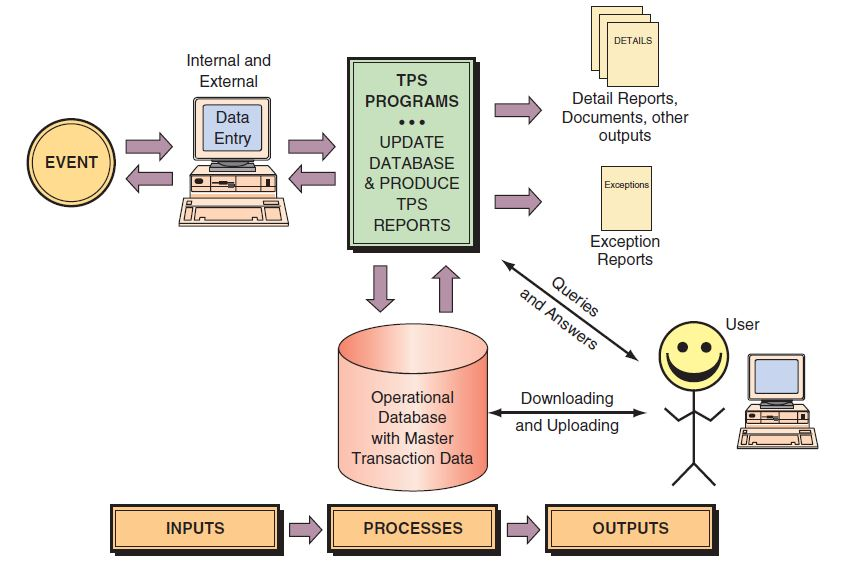
\includegraphics[scale=0.5]{F:/Skripsi/Dokumentasi_Skripsi/Gambar/Teori/tps.JPG}
		{\caption{Alur informasi pada proses transaksi} \cite{Turban:2001}}
	\label{fig:tps}
\end{figure}

Gambar \hyperlink{tps}{2.1} menggambarkan alur dari informasi pada proses transaksi yang akan dijelaskan sebagai berikut : 
\begin{enumerate}
	\item Sistem mencatat semua data yang dibutuhkan dari sebuah kejadian.
	\item Data kemudian disimpan ke dalam \textit{database}, apabila data tersebut belum terdapat pada \textit{database} maka akan dilakukan operasi \textit{insert} \textit{record} baru, sementara apabila data tersebut sudah dimiliki oleh \textit{database} maka akan dilakukan operasi \textit{update} untuk memperbaharui informasi pada \textit{record} yang sudah ada tersebut dengan informasi dari data baru.
	\item Apabila \textit{record} pada \textit{database} sudah berhasil ditambahkan/diperbaharui, program dapat menghasilkan laporan maupun dokumen yang dapat digunakan oleh pihak organisasi maupun dapat diakses oleh pihak luar.
\end{enumerate}

\textbf{Karakteristik TPS}\
\label{sec:karakteristik_tps}
Berikut ini akan dijelaskan karakteristik dari TPS, antara lain \cite{Turban:2001} : 
\begin{enumerate}
	\item Volume data yang diproses sangat besar.
	\item Sumber data umumnya berasal dari dalam perusahaan dan keluaran yang dihasilkan dimaksudkan untuk pihak dalam perusahaan.
	\item Pemrosesan informasi dilakukan secara teratur. Misal harian, mingguan, dan sebagainya.
	\item Dibutuhkan kapasitas penyimpan (basis data) yang besar.
	\item Dibutuhkan kecepatan pemrosesan yang tinggi karena volume data yang diolah juga besar.
	\item Umumnya sistem memantau dan mengumpulkan data yang telah di-\textit{input} sebelumnya.
	\item Jenis data masukan dan keluaran sudah terstruktur. Karena data yang diproses cukup stabil, data diformat dalam suatu standar.
	\item Level kerincian yang tinggi terutama pada masukan tetapi seringkali juga pada keluaran.
	\item Komputasi tidak rumit (menggunakan operasi matematika sederhana atau operasi statistik).
	\item Dibutuhkan tingkat akurasi, integrasi dan keamanan data yang tinggi.
	\item Dibutuhkan tingkat keandalan yang tinggi.
	\item Pengaturan terhadap permintaan merupakan suatu hal wajib. TPS memungkinkan pengguna untuk melakukan \textit{query} terhadap basis data.
\end{enumerate}

\textbf{Contoh Aplikasi TPS}\
\label{sec:contoh_aplikasi _tps}
Berikut ini akan dijelaskan aplikasi-aplikasi apa saja yang memanfaatkan sistem informasi berbentuk TPS berdasarkan fungsinya, yaitu \cite{Laudon:1996} :
\begin{enumerate}
	\item Sistem pemasaran (\textit{Sales})
	\item Sistem produksi (\textit{Manufacturing})
	\item Sistem akuntansi (\textit{Finance})
	\item Sistem ketenaga kerjaan (\textit{HR})
	\item Lain-lain (contoh : universitas)
\end{enumerate}

\subsection{\textit{Office Automation System} (OAS)}
\label{sec:oas}
\textit{Office Automation System} (OAS) adalah aplikasi yang didesain untuk meningkatkan produktivitas pegawai di kantor dengan mendukung koordinasi dan komunikasi antar pegawai \cite{Laudon:1996}. OAS digunakan untuk meningkatkan aliran pekerjaan dan komunikasi antar sesama pegawai, tidak peduli apakah pekerja tadi berada di satu lokasi yang sama ataupun tidak sehingga tingkat produktivitas pegawai dapat meningkat.

\textbf{Dampak dari Otomatisasi}\
Otomatisasi proses dapat membawa dampak positif pada organisasi yang menerapkannya. Dampak dari otomatisasi terbagi menjadi 3 tingkatan yaitu \cite{Susan:1982}: 
\begin{enumerate}
	\item \textit{Innovative}\\
	Tingkat ini merupakan tahap awal dari otomatisasi. Pada level ini organisasi mulai menerapkan metode baru, penggunaan \textit{tools} dan teknik dalam pengerjaan beberapa tugasnya. Dampak otomatisasi pada level ini ditandai dengan tumbuhnya dan berkembangannya sektor bisnis.
	\item \textit{Rective}\\
	Tingkat ini organisasi mulai meningkatkan dukungan dan fasilitas untuk para manajer dan pegawai, kontorl sistem yang lebih baik dari sebelumnya dan semakin mudahnya mengakses suatu informasi yang akurat. Dampaknya produktivitas pegawai akan meningkat.
	\item \textit{Routine}\\
	Tingkat ini merupakan level teratas dari otomatisasi proses. Pada level ini hampir semua tugas yang ada pada organisasi sudah sebagian besar diotomatisasi. Dampaknya akan terasa pada berkurangnya biaya produksi dan peningkatan pada muatan pekerjaan dari staf pendukung.
\end{enumerate}
 
\section{\LaTeX}
\label{sec:latex}
\LaTeX adalah sebuah bahasa markup untuk sistem penulisan dokumen yang dikembangkan oleh Leslie B. Lamport dan dirilis pada tahun 1985 \cite{Lamport:1994} . \LaTeX memiliki filosofi WYMIWYG (What You Mean Is What You Get) yang berarti sesuatu yang akan kita tulis akan ditulis berdasarkan arti dari hal tersebut. Oleh karena itu, untuk menambahkan suatu perintah pada dokumen yang sedang kita tulis perlu menambahkan suatu \textit{command}. \textit{Command} adalah kata spesial yang menentukan suatu sifat pada \LaTeX. Hampir semua \textit{command} pada \LaTeX selalu diawali dengan tanda \textbackslash dan beberapa \textit{command} memiliki parameter. Parameter diawali dengan tanda kurung kurawal buka dan diakhiri denga kurung kurawal tutup(\{\}). File \LaTeX memiliki ekstensi .tex.  

Untuk menulis dokumen pada \LaTeX dibutuhkan beberapa \textit{command} yang wajib ada dalam sebuah dokumen, yaitu \cite{Lamport:1994} : 
\begin{enumerate}
	\item \texttt{\string\documentclass[option]\{class\}}\\
	Digunakan untuk menentukan jenis dokumen dan \textit{layout} dokumen. Bagian \textit{option} dapat dikosongkan atau dapat digunakan untuk menyimpan pilihan pengaturan \textit{layouting}. Pada bagian \textit{class} digunakan untuk menentukan tipe dokumen yang akan dibuat.
	\item \texttt{\string\usepackage\{package name\}}\\
	Digunakan untuk menambahkan sebuah \textit{package} baru untuk mendukung pembuatan dokumen. Package adalah sebuah pengaturan yang berisi sekumpulan \textit{command} dan pengaturan yang akan digunakan untuk mengatur keseluruhan isi dokumen. \textit{Package name} diisi dengan nama \textit{package} yang akan digunakan.
	\item \texttt{\string\title\{\}}\\
	Digunakan untuk menapilkan halaman judul. Biasanya halaman judul akan memuat judul dokumen, nama pengarang dan tanggal pembuatan dokumen. Nama pengarang dan tanggal pembuatan dapat ditampilkan dengan menambahkan perintah \texttt{\string\author\{nama\}} dan \texttt{\string\date\{tanggal\}}
	\item \texttt{\string\begin\{document\}}...\texttt{\string\end\{document\}}\\
	Digunakan untuk mengawali dan mengakhiri isi dokumen.
\end{enumerate}

\subsection{Mailmerge}
\label{sec:mailmerge}
\textit{Mailmerge} adalah salah satu \textit{package} yang disediakan oleh \LaTeX yang berupa antar muka untuk pembuatan surat atau dokumen. \textit{Mailmerge} memilik 2 komponen utama yaitu \textit{repeated text} yaitu sejumlah tulisan dalam dokumen tersebut yang ditulis sama persis berulang kali pada setiap pengulangan, dan \textit{command} yang dapat diganti-ganti dengan suatu nilai tertentu pada setiap pengulangan \cite{Frasson:2009} .\

Untuk menggunakan \textit{package mailmerge}, ada beberapa \textit{command} yang perlu ditambahkan seperti \cite{Frasson:2009} :
\begin{enumerate}
	\item \texttt{\string\mailfields}\\
	Digunakan untuk menyatakan nama \textit{field} yang akan digunakan. Nama \textit{field} disimpan di dalam parameter \texttt{\string\mailfields}. Urutan nama \textit{field} yang dideklarasikan akan berpengaruh pada \texttt{\string\mailentry}. Nama field akan menjadi parameter bagi \textit{command} \texttt{\string\field}.
	\item \texttt{\string\mailrepeat}\\
	Digunakan untuk menentukan teks mana saja yag diulang setiap kali pengulangan. Teks yang akan diulang maupun \textit{command} \texttt{\string\field} akan menjadi parameter bagi \texttt{\string\mailrepeat}, namun isi dari \textit{command} \texttt{\string\field} akan berubah pada setiap kali pengulangan sesuai dengan data pada \textit{entry}.
	\item \texttt{\string\mailentry}\\
	Digunakan untuk penampungan nilai sebelum dimasukkan sebagai parameter \textit{command} \texttt{\string\field}.
\end{enumerate}
	Berikut ini adalah urutan tata letak setiap command untuk pembuatan mailmerge :
	\begin{verbatim}
    \usepackage{ifthen,mailmerge}

    % \ifequal{A}{B}{what if A=B}{what if A<>B}
    \newcommand{\ifequal}[2]{\ifthenelse{\equal{#1}{#2}}}

    \mailfields{name,friends,drives}

    \mailrepeat{\section*{\field{name}'s profile}

       \field{name} has
       \ifequal{\field{friends}}{}
         {no friends}
         {\field{friends} as friends}.
       \ifequal{\field{drives}}{yes}{Drives.}{Doesn't drive.}

    (entry \entrynumber\ of \numberofentries)

    % \newpage optional
    }

    \mailentry{John,{Bart and Robert},yes}
    \mailentry{Sara,{Jean, Phillip and Maria},no}
    \mailentry{Edward,,yes}
 \end{verbatim}}{}
\ifdefstring{\vbabc}{1}{\chapter{Analisis}
\label{chap:analisis}
Analisis membahas mengenai deskripsi sistem terkini, hasil survey aplikasi sejenis dan analisis sistem usulan.

\section{Deskripsi Sistem Terkini}
\label{sec:deskripsi_sistem_terkini}
Deskripsi sistem terkini membahas mengenai gambaran umum institusi, jenis-jenis surat akademik yang dikeluarkan oleh pihak TU, prosedur pemesanan surat akademik, prosedur pembuatan surat akademik, prosedur pengambilan surat akademik dan analisis kebutuhan. \\

\subsection{Gambaran Umum Institusi}
\label{sec:gambaran_umum_institusi}
Fakultas Teknologi Informasi dan Sains (FTIS) adalah salah satu fakultas yang terdapat di kampus Universitas Katolik Parahyangan (Unpar). FTIS dikepalai oleh seorang dekan yang dibantu oleh 3 wakil dekan. FTIS memiliki 3 program studi (prodi) yaitu prodi Matematika, Fisika dan Teknik Informatika. Setiap program studi dipimpin oleh seorang ketua prodi yang dibantu oleh seorang sekretaris prodi, kecuali jurusan fisika. Setiap prodi, kecuali prodi matematika, memiliki laboratorium yang dikepalai oleh seorang kepala laboratorium. Untuk mengurusi masalah administrasi fakultas, terdapat bagian Tata Usaha (TU) yang terdiri dari sub bagian (subag) tertentu yang mengurusi bidang tertentu.\

Gambar \hyperlink{organigram_fakultas}{3.1} menjelaskan struktur organisasi dari FTIS. Di bawah ini akan dijelaskan  setiap bagian dari struktur organisasi tersebut. Setiap fungsi pada struktur organisasi tersebut memiliki tugas, wewenang, dan tanggung jawab yang berbeda.
\begin{figure}[H]
	\centering
		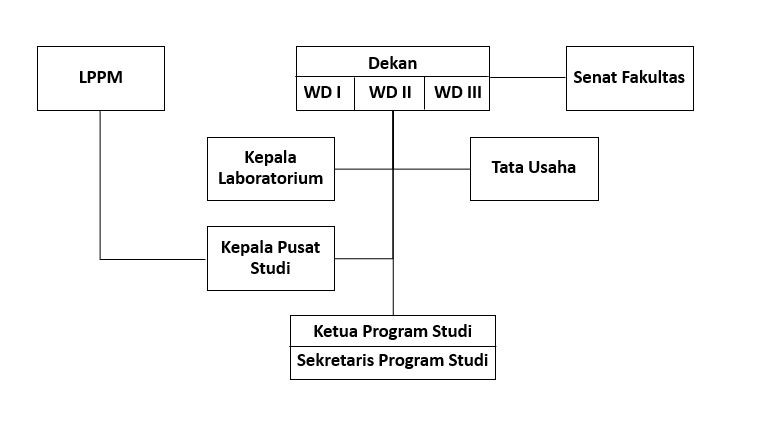
\includegraphics[scale=0.65]{F:/Skripsi/Template/Gambar/Diagram/sistem_terkini/organigram/organigram_fakultas.JPG}
	\caption{Struktur Organisasi Fakultas Teknologi Informasi dan Sains}
	\label{fig:organigram_fakultas}
\end{figure}

\begin{enumerate}
	\item Dekan \\
	berfungsi sebagai pengambil keputusan tertinggi di fakultas.
	\item Senat Fakultas \\
	berfungsi sebagai partner dekan untuk membantu memberikan pertimbangan dari keputusan yang akan diambil. Senat dipilih dari dosen tetap di fakultas.
	\item Wakil Dekan Bidang Akademik (WD I)\\
	berfungsi untuk membantu dekan pada pengambilan segala keputusan yang berhubungan dengan kegiatan akademik yang berlangsung di setiap program studi yang ada pada fakultas.
	\item Wakil Dekan Bidang Sumber Daya (WD II)\\
	berfungsi untuk membantu dekan pada pengambilan segala keputusan yang berhubungan dengan pengelolaan setiap bentuk sumber daya yang terdapat di lingkungan fakultas.
	\item Wakil Dekan Bidang Kemahasiswaan dan Alumni (WD III)\\
	berfungsi untuk membantu dekan pada pengambilan segala keputusan yang berhubungan dengan setiap permasalahan kemahasiswaan dan alumni di lingkungan fakultas.
	\item Kepala Laboratorium \\
	bertanggung jawab akan perawatan dan operasional laboratorium.
	\item Ketua Program Studi \\
	berfungsi sebagai pengambil keputusan tertinggi di lingkungan program studi.
	\item Sekretaris Program Studi \\
	berfungsi untuk membantu ketua program studi pada pengambilan segala keputusan di lingkungan program studi.
	\item Tata Usaha \\
	berfungsi untuk melayani segala kegiatan administrasi yang terjadi di lingkungan FTIS.
	\item LPPM (Lembaga Penelitian \& Pengabdian kepada Masyarakat)\\
	berfungsi sebagai lembaga yang mengakomodasi penelitian dan pengabdian ilmu pengetahuan.
	\item Kepala Pusat Studi \\
	merupakan bagian kecil dari LPPM yang berfungsi untuk menerapkan Tridharma Perguruan Tinggi, namun lebih spesifik kepada suatu bidang studi.
\end{enumerate}

Gambar \hyperlink{organigram_TU}{3.2} merupakan struktur organisasi dari TU FTIS. Bagian tata usaha dipimpin oleh seorang Kepala Bagian (Kabag). Di bawah Kabag terdapat 4 sub bagian (Subag) yang dikepalai oleh seorang Kepala Sub Bagian (Kasubag). Berikut ini akan dijelaskan struktur organisasi yang ada di tata usaha FTIS.
\begin{figure}[H]
	\centering
		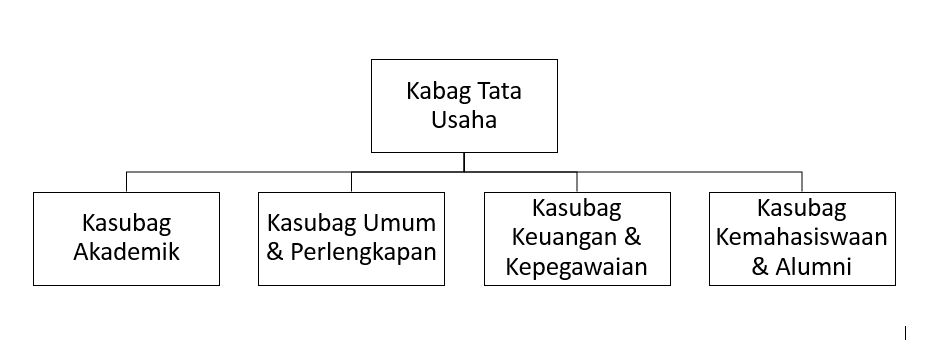
\includegraphics[scale=0.35]{F:/Skripsi/Template/Gambar/Diagram/sistem_terkini/organigram/organigram_TU.JPG}
	\caption{Struktur Organisasi Tata Usaha Fakultas Teknologi Informasi dan Sains}
	\label{fig:organigram_TU}
\end{figure}
\begin{enumerate}
	\item Kabag Tata Usaha \\
	berfungsi sebagai pemegang keputusan tertinggi di tata usaha.
	\item Kasubag Akademik \\
	berfungsi sebagai pengatur segala hal yang berhubungan dengan kegiatan akademik di lingkungan fakultas, seperti pengaturan jadwal kuliah dan ujian, jadwal perwalian, pembagian ruangan, memperbanyak dan mendistribusikan soal ujian, dll.
	\item Kasubag Umum dan Peralatan \\
	berfungsi sebagai pengatur segala kegiatan, sarana dan prasarana yang ada di lingkungan fakultas. 
	\item Kasubag Keuangan dan Kepegawaian \\
	berfungsi sebagai pengatur operasional keuangan dan kepegawaian di lingkungan fakultas.
	\item Kasubag Kemahasiswaan dan Alumni \\
	berfungsi untuk melayani segala keperluan kemahasiswaan dan alumni seperti keperluan surat menyurat, legalisir ijazah, mempersiapkan perlengkapan wisuda, dll.
\end{enumerate}
Berdasarkan uraian mengenai struktur organisasi fakultas, Kasubag Kemahasiswaan dan Alumni berperan mengurusi keperluan surat menyurat di fakultas. Surat-surat yang dibuat termasuk juga dengan surat akademik yang akan dibahas lebih detil pada subbab selanjutnya.

\subsection{Jenis-Jenis Surat Akademik}
\label{sec:jenis_jenis_surat_akademik}
Ada berbagai macam surat akademik yang dikeluarkan oleh TU FTIS. Surat yang dikeluarkan antara lain sebagai berikut :
\begin{enumerate}
	\item Surat perwalian yang diwakilkan. \\
	Surat ini berlaku apabila mahasiswa yang bersangkutan berhalangan hadir untuk melakukan perwalian dengan dosen wali sehingga diwakilkan kepada mahasiswa lain yang diberi kuasa.
	
	\item Surat izin cuti studi. \\
	Surat ini berlaku apabila mahasiswa yang bersangkutan tidak akan mengikuti perkuliahan pada semester tertentu. Biasanya surat ini digunakan apabila mahasiswa mengalami sakit keras dan membutuhkan masa penyembuhan yang lama ataupun tidak ada mata kuliah yang dibuka pada semester yang berjalan. Surat ini dapat diproses apabila mahasiswa pemohon telah memenuhi 2 syarat, yaitu tidak memiliki tunggakan pembayaran uang kuliah dan sudah membayar uang cuti studi.
	
	\item Surat dispensasi pembayaran. \\
	Surat ini berlaku apabila mahasiswa yang bersangkutan berencana mengambil mata kuliah kurang dari 10 sks pada semester yang akan ditempuh. Surat ini harus diproses sebelum masa FRS berlangsung. Surat ini berbentuk formulir isian. Pertama mahasiswa harus mengisi formulir. Setelah formulir diisi sesuai dengan data yang dibutuhkan, formulir akan diteruskan kepada dosen wali dari mahasiswa yang bersangkutan melalui Petugas TU untuk mendapatkan tanda tangan dosen wali. Setelah mendapat tanda tangan dosen wali, formulir diteruskan kepada Biro Keuangan Unpar untuk mendapatkan persetujuan. Apabila disetujui, akan dikirimkan surat persetujuan kepada Petugas TU untuk mengubah jumlah tagihan pembayaran uang kuliah milik mahasiswa di situs \textit{studentportal}. Sehingga jumlah tagihan yang muncul akan sesuai dengan sks mata kuliah yang akan diambil. 
	
	\item Surat pengajuan pengambilan kelebihan pembayaran uang kuliah (tunai). \\
	Surat ini berlaku apabila mahasiswa yang bersangkutan telah membayar uang kuliah sesuai dengan sks mata kuliah yang diambil namun kemudian membatalkan mata kuliah yang telah diambil tersebut. Surat ini berbentuk formulir isian. Pertama mahasiswa harus mengisi formulir. Setelah formulir diisi sesuai dengan data yang dibutuhkan, formulir akan ditandatangani oleh Petugas TU. Setelah ditandatangani, formulir diteruskan kepada Biro Keuangan Unpar untuk diproses. Setelah diproses akan dikirimkan surat keterangan pengembalian uang kuliah beserta sejumlah uang kelebihan pembayaran kuliah kepada Petugas TU. Uang akan diberikan kepada mahasiswa pemohon dan surat keterangan akan disimpan di TU sebagai arsip.
	
	\item Surat izin pengunduran diri mahasiswa. \\
	Surat ini berfungsi sebagai surat pernyataan apabila seorang mahasiswa hendak mengundurkan diri dari Unpar. Biasanya lasan pengambilan surat ini dikarenakan mahasiswa yang bersangkutan merasa tidak cocok dengan jurusan atau telah diterima di universitas lain dan hendak berkuliah di universitas tersebut.
	
	\item Surat keterangan. \\
	Surat ini memiliki fungsi yang beragam. Surat ini dapat digunakan untuk pernyataan mahasiswa aktif, pembuatan surat kelakuan baik, membuka rekening, membuat visa, dll.
	
	\item Surat penundaan pembayaran uang kuliah. \\
	Surat ini berlaku apabila mahasiswa yang bersangkutan belum bisa membayar uang kuliah sampai tanggal yang telah ditentukan. Fungsi surat ini yaitu untuk memberikan kelonggaran waktu pembayaran uang kuliah pada mahasiswa sehingga mahasiswa yang bersangkutan akan terlepas dari denda keterlambatan pembayaran. Pertama mahasiswa harus mengisi formulir. Setelah formulir diisi sesuai dengan data yang dibutuhkan, akan dibuatkan surat yang kemudian diteruskan kepada Wakil Dekan Bidang Sumber Daya melalui Petugas TU untuk mendapatkan tanda tangan wakil dekan. Setelah mendapat tanda tangan wakil dekan, surat diteruskan kepada Biro Keuangan Unpar untuk mendapatkan persetujuan. Apabila disetujui, akan dikirimkan surat persetujuan kepada Petugas TU yang menyatakan pemberian izin kepada mahasiswa pemohon untuk menunda pembayaran uang kuliah.
	
	\item Surat izin studi lapangan. \\
	Surat ini berfungsi sebagai surat pengantar apabila ada mahasiswa yang hendak melakukan wawancara, survei, studi banding atau observasi ke sebuah instansi.
	
	\item Surat permohonan beasiswa. \\
	Surat ini berfungsi apabila seorang mahasiswa hendak mengajukan beasiswa kepada universitas maupun fakultas. Surat ini berbentuk formulir isian. Setelah formulir diisi sesuai dengan data yang dibutuhkan, formulir diteruskan kepada dosen wali mahasiswa pemohon untuk mendapat catatan dan tanda tangan dosen wali. Setelah itu surat akan diteruskan kepada dekan untuk catatan dan tanda tangan dekan. Setelah semua data terisi lengkap, formulir akan diserahkan kepada Badan Kemahasiswaan dan Alumni Unpar.
	
	\item Surat keterangan beasiswa. \\
	Surat ini berfungsi sebagai surat pernyataan bahwa mahasiswa yang bersangkutan telah menerima beasiswa dari pihak non-Unpar dan tidak menerima beasiswa lain yang berasal dari Unpar.
\end{enumerate}

\subsection{Prosedur Pemesanan Surat}
\label{sec:prosedur_pemesanan_surat}
Gambar \hyperlink{pemesanan_terkini}{3.3} merupakan prosedur pemesanan surat yang dilakukan oleh mahasiswa kepada Kasubag Kemahasiswaan dan Alumni. Untuk selanjutnya Kasubag Kemahasiswaan dan Alumni akan disebut sebagai Petugas TU untuk mempersingkat penyebutan nama. Prosedur pemesanan surat dimulai dengan:
\begin{enumerate}
	\item Mahasiswa mendatangi Petugas TU dan menyebutkan surat yang dibutuhkan.
	\item Petugas TU memberikan formulir yang harus diisi sesuai dengan surat yang dibutuhkan.
	\item Mahasiswa mengisi formulir.
	\item Mahasiswa mengembalikan formulir ke Petugas TU.
	\item Petugas TU mengecek pengisian formulir. Apabila ada kesalahan pengisian, maka formulir dikembalikan kepada mahasiswa untuk diperbaiki. Jika tidak ada kesalahan maka dapat lanjut ke proses berikutnya.
	\item Apabila sedang tidak ada pesanan surat, surat dapat langsung dibuatkan, apabila ada pesanan, surat akan masuk \textit{waiting list} dan Petugas TU akan memberikan estimasi waktu selesai pengerjaan surat.
\end{enumerate}

\begin{figure}[H]
	\centering
		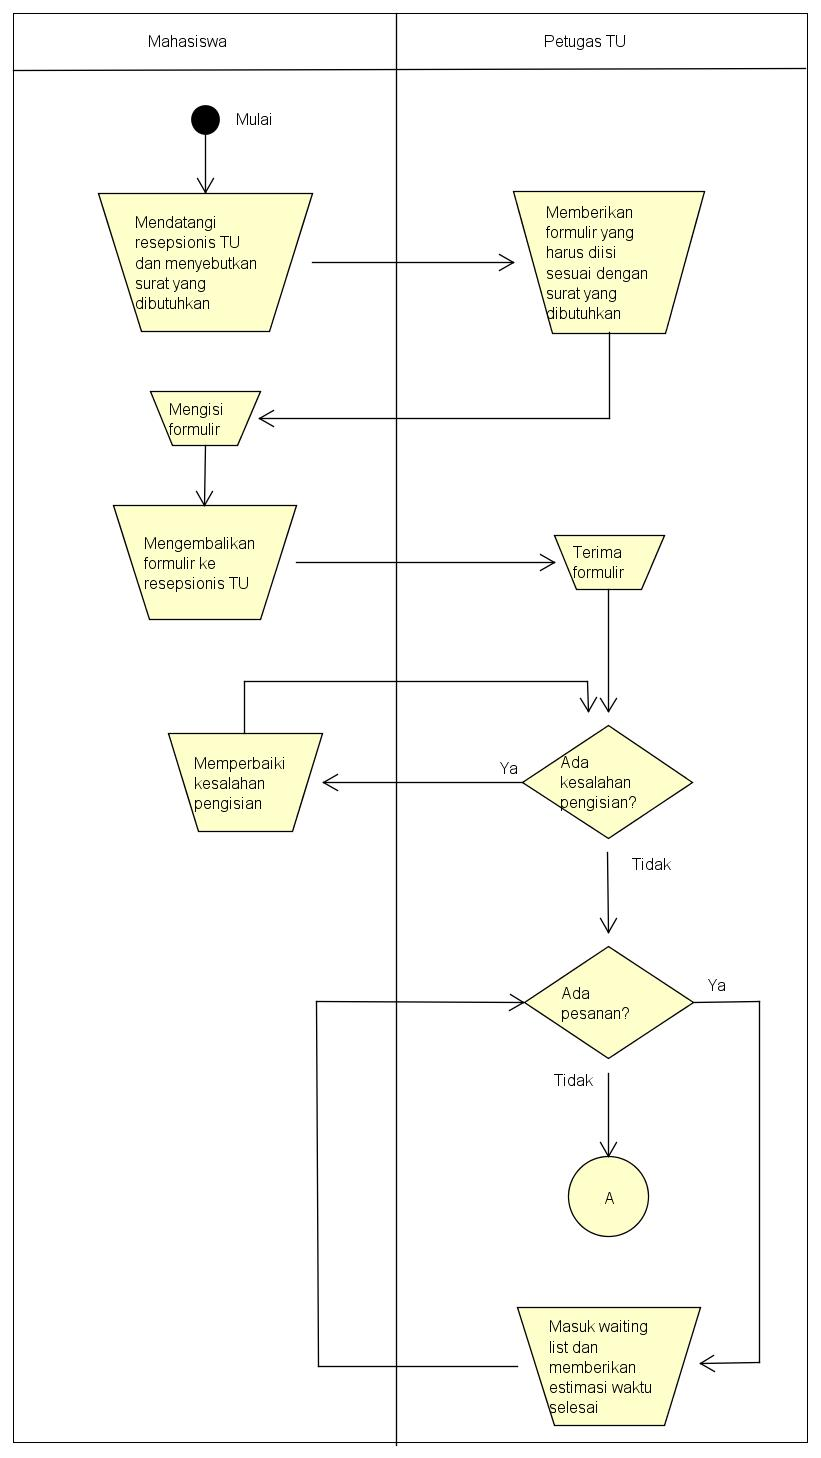
\includegraphics[scale=0.30]{F:/Skripsi/Template/Gambar/Diagram/sistem_terkini/work_flow/pemesanan_terkini.jpg}
	{\caption{Prosedur pemesanan surat terkini}}
	\label{fig:pemesanan_terkini}
\end{figure}

\subsection{Prosedur Pembuatan Surat}
\label{sec:prosedur_pembuatan_surat}
Gambar \hyperlink{pembuatan_terkini}{3.4} merupakan prosedur pembuatan surat yang dilakukan oleh Petugas TU. Prosedur pembuatan surat dimulai dengan:
\begin{enumerate}
	\item Petugas TU mengecek formulir yang telah diisi oleh mahasiswa.
	\item Petugas TU membuka \textit{template} surat yang dipesan.
	\item Petugas TU memasukkan semua data yang telah dituliskan oleh mahasiswa pada formulir ke \textit{template}.
	\item Petugas TU melakukan cek ulang apabila terjadi kesalahan dalam memasukkan data.
	\item Apabila tidak ada kesalahan Petugas TU dapat langsung mencetak surat.
	\item Petugas akan menghubungi pejabat tertentu yang memiliki keterkaitan dengan surat yang sedang diproses untuk mendapatkan tanda tangan dari pejabat yang bersangkutan.
	\item Apabila mahasiswa pemohon menunggu di sekitar ruang TU maka surat dapat langsung diambil oleh mahasiswa pemohon. Apabila tidak ada, maka surat akan disimpan oleh Petugas TU.
\end{enumerate}

\begin{figure}[H]
	\centering
		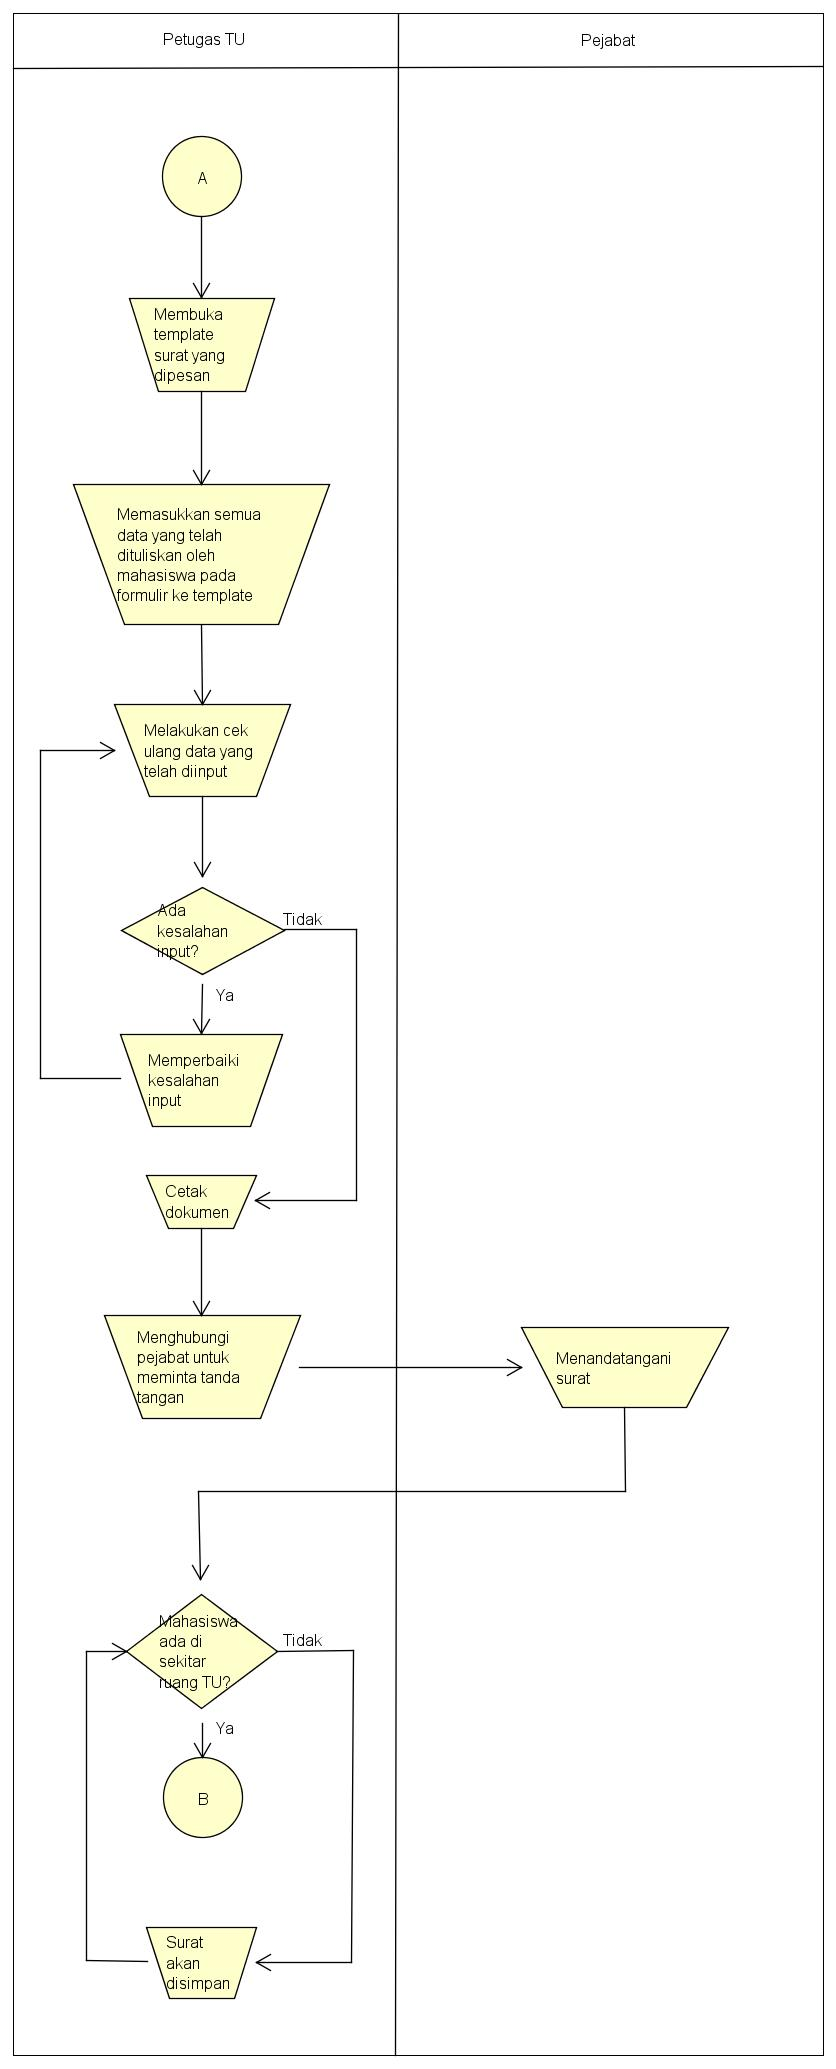
\includegraphics[scale=0.25]{F:/Skripsi/Template/Gambar/Diagram/sistem_terkini/work_flow/pembuatan_terkini.jpg}
	{\caption{Prosedur pembuatan surat terkini}}
	\label{fig:pembuatan_terkini}
\end{figure}

\subsection{Prosedur Pengambilan Surat}
\label{sec:prosedur_pengambilan_surat}
Gambar \hyperlink{pengambilan_terkini}{3.5} merupakan prosedur pengambilan surat yang dilakukan oleh mahasiswa kepada Petugas TU. Prosedur pengambilan surat dimulai dengan:
\begin{enumerate}
	\item Mahasiswa yang memesan mendatangi Petugas TU dan menyebutkan surat apa yang telah dipesan.
	\item Petugas TU memberikan surat yang telah dicetak kepada mahasiswa.
\end{enumerate}

\begin{figure}[H]
	\centering
		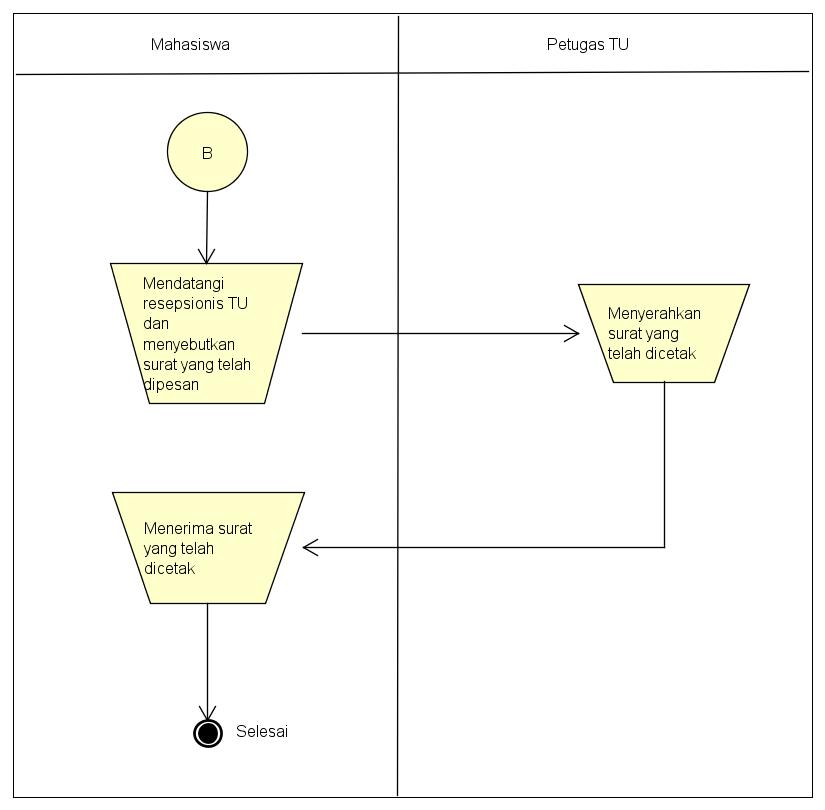
\includegraphics[scale=0.35]{F:/Skripsi/Template/Gambar/Diagram/sistem_terkini/work_flow/pengambilan_terkini.jpg}
	{\caption{Prosedur pengambilan surat terkini}}
	\label{fig:pengambilan_terkini}
\end{figure}

\subsection{Analisis Kebutuhan}
\label{sec:analisis_kebutuhan}
Berdasarkan paparan yang telah disebutkan di atas, maka ditemukan beberapa masalah yang menjadi fokus utama dari penelitian ini. Masalah-masalah yang telah ditemukan antara lain:
\begin{enumerate}
	\item Pemesanan surat akademik tidak bisa dilakukan mendadak.
	\item Petugas bisa kewalahan apabila permintaan surat yang masuk cukup banyak dalam sehari.
	\item Ada kemungkinan kesalahan pemasukan data dari formulir ke komputer.
\end{enumerate}

\section{Hasil Survey Aplikasi Sejenis}
\label{sec:hasil_survey_aplikasi_sejenis}
Berdasarkan survey yang telah dilakukan terhadap beberapa universitas di Bandung, seperti Institut Teknologi Bandung (ITB) dan Universitas Pendidikan Indonesia (UPI), tidak ditemukan adanya penggunaan aplikasi yang khusus untuk menangani kebutuhan surat akademik. Penanganan surat akademik masih dilakukan secara konvensional yaitu dengan mendatangi dosen wali terlebih dahulu dan apabila sudah mendapat persetujuan dari dosen wali maka mahasiswa dapat membuat surat akademik dibantu oleh tata usaha di fakultas masing-masing.

\section{Analisis Sistem Usulan}
\label{sec:analisis_sistem_usulan}
Analisis sistem usulan membahas mengenai prosedur pembuatan surat usulan, diagram \textit{usecase}, \textit{task scenario}, analisis kebutuhan data dari surat, dan diagram ER. \\

\subsection{Surat-surat Yang Dapat Ditangani}
\label{sec:surat_yang_ditangani}
Dari 10 surat yang telah disebutkan di atas, diambil 7 surat saja yang akan dibahas lebih lanjut pada penelitian ini. Hal ini dikarenakan 6 surat tersebut dapat menghasilkan surat yang kemudian akan dikembalikan kepada mahasiswa yang bersangkutan untuk kemudian disampaikan kepada lembaga yang membutuhkan surat tersebut. Keenam surat tersebut yaitu :
\begin{enumerate}
	\item Surat keterangan beasiswa. \\
	Surat pernyataan bahwa mahasiswa ybs. tidak menerima beasiswa dari pihak universitas maupun fakultas dan hanya menerimah beasiswa dari satu organisasi.
	\item Surat keterangan mahasiswa aktif. \\
	Surat pernyataan bahwa mahasiswa ybs. merupakan mahasiswa aktif Fakultas Teknologi Informasi dan Sains Uiversitas Katolik Parahyangan.
	\item Surat pengantar pembuatan visa. \\
	Surat yang pengantar yang diajukan mahasiswa kepada suatu kedutaan besar negara asing dengan tujuan untuk untuk membuat visa.
	\item Surat izin studi lapangan. \\
	Surat izin yang diajukan apabila seorang mahasiswa hendak melakukan penelitian ke suatu organisasi dan membutuhkan surat pengantar dari fakultas sebagai syarat penelitian. Surat ini dapat digunakan untuk perorangan maupun kelompok. Untuk surat izin studi lapangan kelompok, dapat mewakili 1 orang ketua dan maksimal 4 orang anggota.
	\item Surat perwalian yang diwakilkan. \\
	Surat yang diajukan oleh mahasiswa apabila mahasiswa ybs. berhalangan hadir pada saat perwalian dan hendak diwakilkan oleh mahasiswa lain. 
	\item Surat izin cuti studi. \\
	Surat yang diajukan oleh mahasiswa apabila mahasiswa ybs. hendak mengambil cuti studi pada semester tertentu. Surat ini memerlukan lampiran dari orang tua/wali untuk
	\item Surat izin pengunduran diri mahasiswa. \\
	Surat yang diajukan oleh mahasiswa apabila mahasiswa ybs. hendak mengundurkan diri dari Fakultas Teknologi Informasi dan Sains Uiversitas Katolik Parahyangan.
\end{enumerate}

\subsection{Prosedur Pembuatan Surat Usulan}
\label{sec:pembuatan_surat_usulan}
Gambar \hyperlink{pembuatan_usulan}{3.6} merupakan prosedur pembuatan surat yang dilakukan oleh mahasiswa. Pada prosedur usulan ini, untuk membuat surat akademik tidak perlu melalui 3 tahapan seperti yang dijelaskan pada subbagian sistem terkini. Prosedur pembuatan surat dimulai dengan:
\begin{enumerate}
	\item Mahasiswa melakukan login
	\item Mahasiswa memilih jenis surat yang akan dibuat
	\item Mahasiswa memasukkan data yang dibutuhkan dengan benar
	\item Mahasiswa mengklik tombol \textit{preview} untuk melihat surat secara keseluruhan
	\item Apabila terdapat kesalahan pada pengisian data, mahasiswa dapat mengklik tombol \textit{edit} untuk memperbaiki kesalahan pada pengisian data.
	\item Apabila tidak ada kesalahan, mahasiswa dapat mengklik tombol \textit{process} untuk meng-\textit{generate} \textit{file} .pdf dan men-\textit{download} \textit{file} tersebut.
	\item Setelah mendapatkan \textit{file} .pdf surat, mahasiswa dapat mencetak surat.
	\item Setelah surat dicetak, mahasiswa memberikan surat tersebut kepada Petugas TU untuk ditanda tangani oleh pejabat yang berkaitan dengan surat.
	\item Setelah surat ditanda tangani, Petugas TU mengembalikan surat yang sudah ditanda tangani tersebut kepada mahasiswa.
	\
\end{enumerate}
\begin{figure}[H]
	\centering
		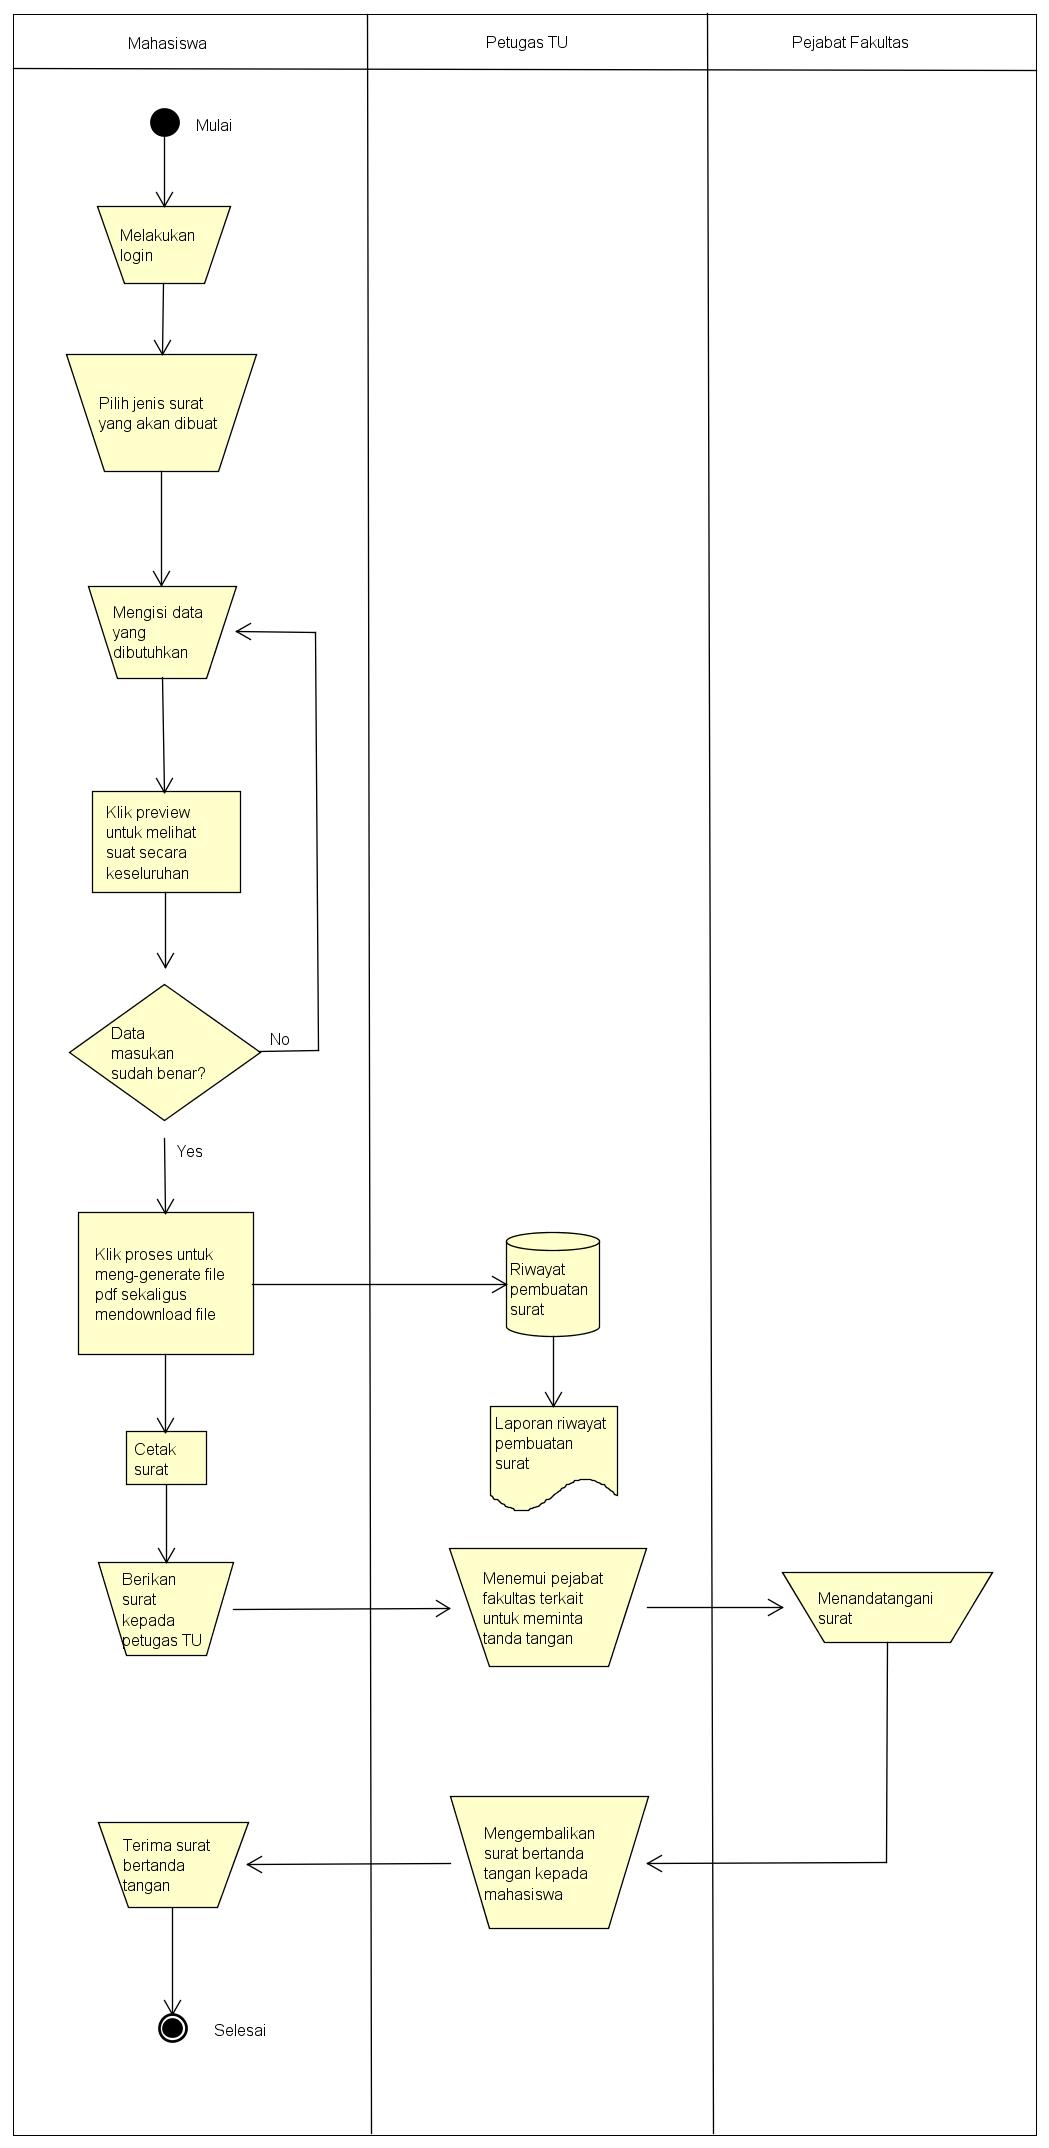
\includegraphics[scale = 0.27]{F:/Skripsi/Template/Gambar/Diagram/sistem_usulan/flowchart/Flowchart0.jpg}
	{\caption{Prosedur pembuatan surat usulan}}
	\label{fig:pembuatan_usulan}
\end{figure}

\subsection{\textit{Data Flow Diagram (DFD)}}
\label{sec:data_flow_diagram}
\textit{Data Flow Diagram (DFD)} adalah diagram untuk memodelkan setiap aliran data pada sistem yang akan dibangun.
Gambar \hyperlink{data_flow}{3.7} merupakan diagram \textit{context} atau DFD \textit{level} 0 yang menjelaskan 
keseluruhan sistem beserta aktornya.

\begin{figure}[H]
	\centering
		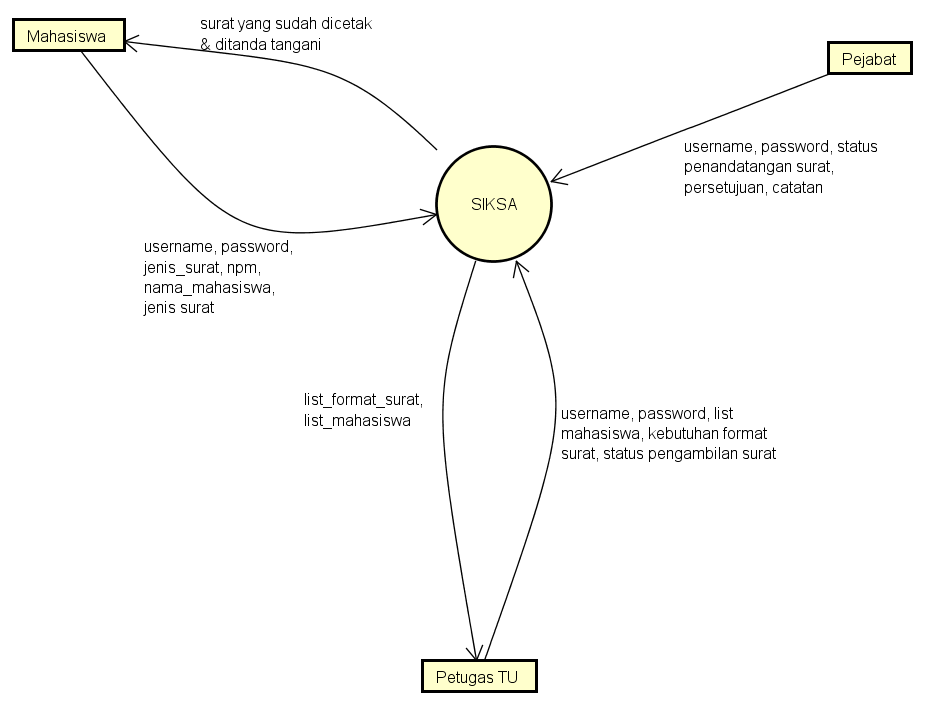
\includegraphics[scale = 0.6]{F:/Skripsi/Template/Gambar/Diagram/sistem_usulan/dfd/Lv0.png}
	\caption{Diagram \textit{context}}
	\label{fig:data_flow}
\end{figure}

\textit{Website} penyedia surat akademik ini memiliki 3 aktor, yaitu \textit{mahasiswa}, \textit{pejabat} dan \textit{petugas TU}. Tiap aktor memiliki hak akses ke beberapa fitur tertentu. Gambar \hyperlink{level_1}{3.8} merupakan DFD \textit{level} 1 yang menjelaskan aliran data pada tiap aktor.

\begin{figure}[H]
	\centering
		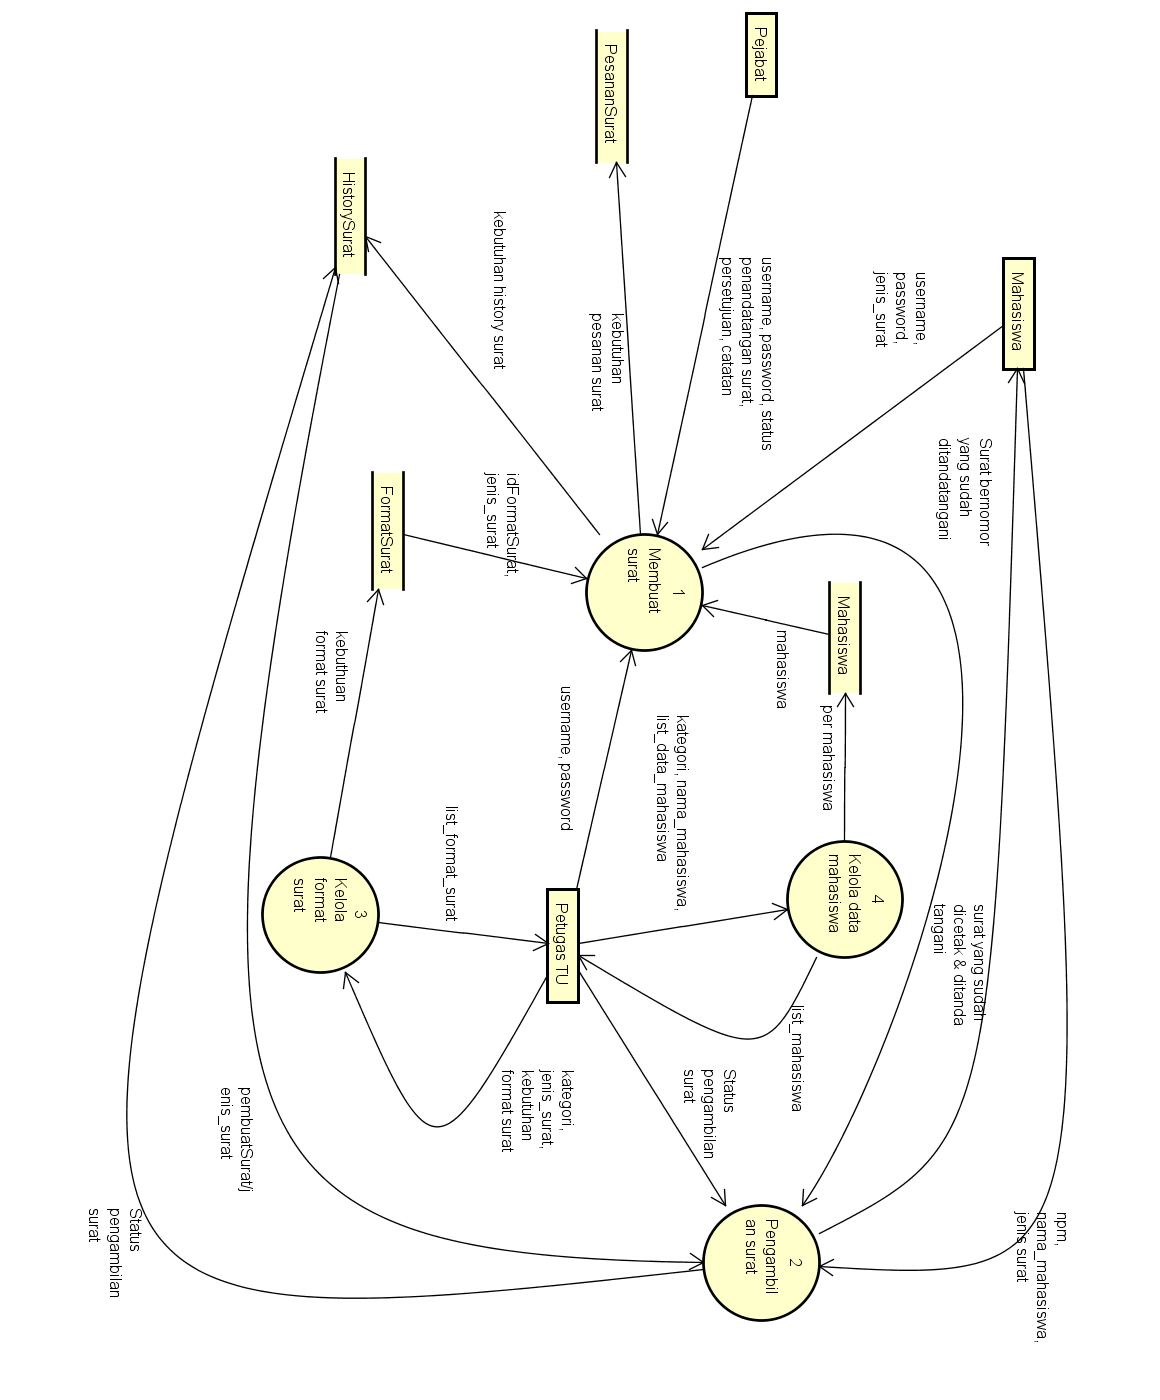
\includegraphics[scale = 0.5]{F:/Skripsi/Dokumentasi_Skripsi/Gambar/Diagram/sistem_usulan/dfd/Lv1-kiri.png}
	\caption{DFD \textit{level} 1}
	\label{fig:level_1}
\end{figure}

Gambar \hyperlink{level_2-1}{3.9} merupakan DFD \textit{level} 2-1 yang menjelaskan aliran data pada saat aktor mahasiswa hendak membuat surat yang kemudian dilanjutkan pada DFD \textit{level} 3-1.10 pada gambar \hyperlink{level_3-1.10}{3.10}

\begin{figure}[H]
	\centering
		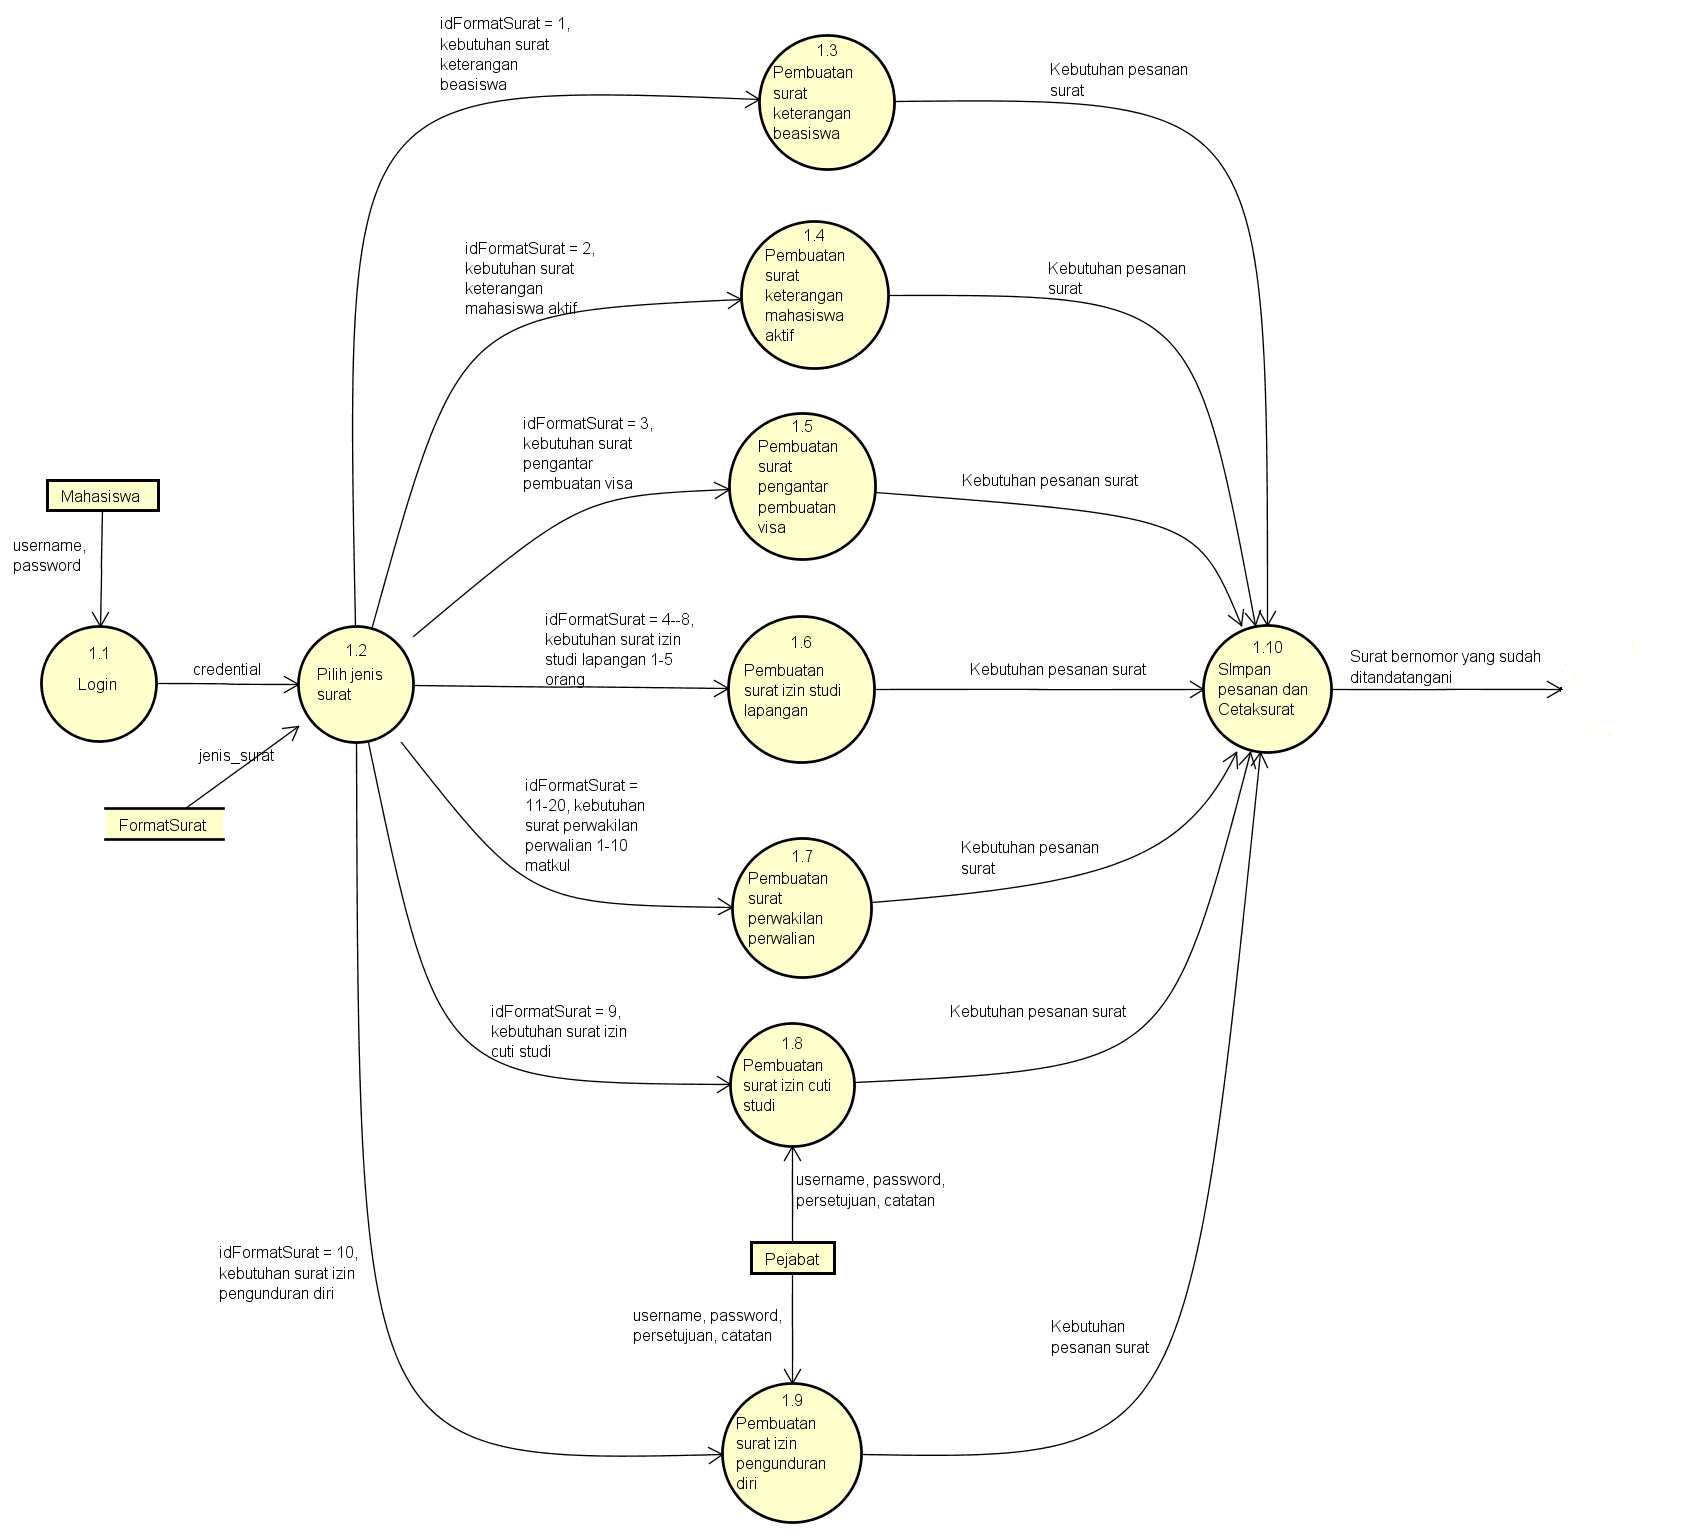
\includegraphics[scale = 0.4]{F:/Skripsi/Dokumentasi_Skripsi/Gambar/Diagram/sistem_usulan/dfd/Lv2-1_buat_suratt.png}
	\caption{DFD \textit{level} 2-1 untuk pembuatan surat}
	\label{fig:level_2-1}
\end{figure}

\begin{figure}[H]
	\centering
		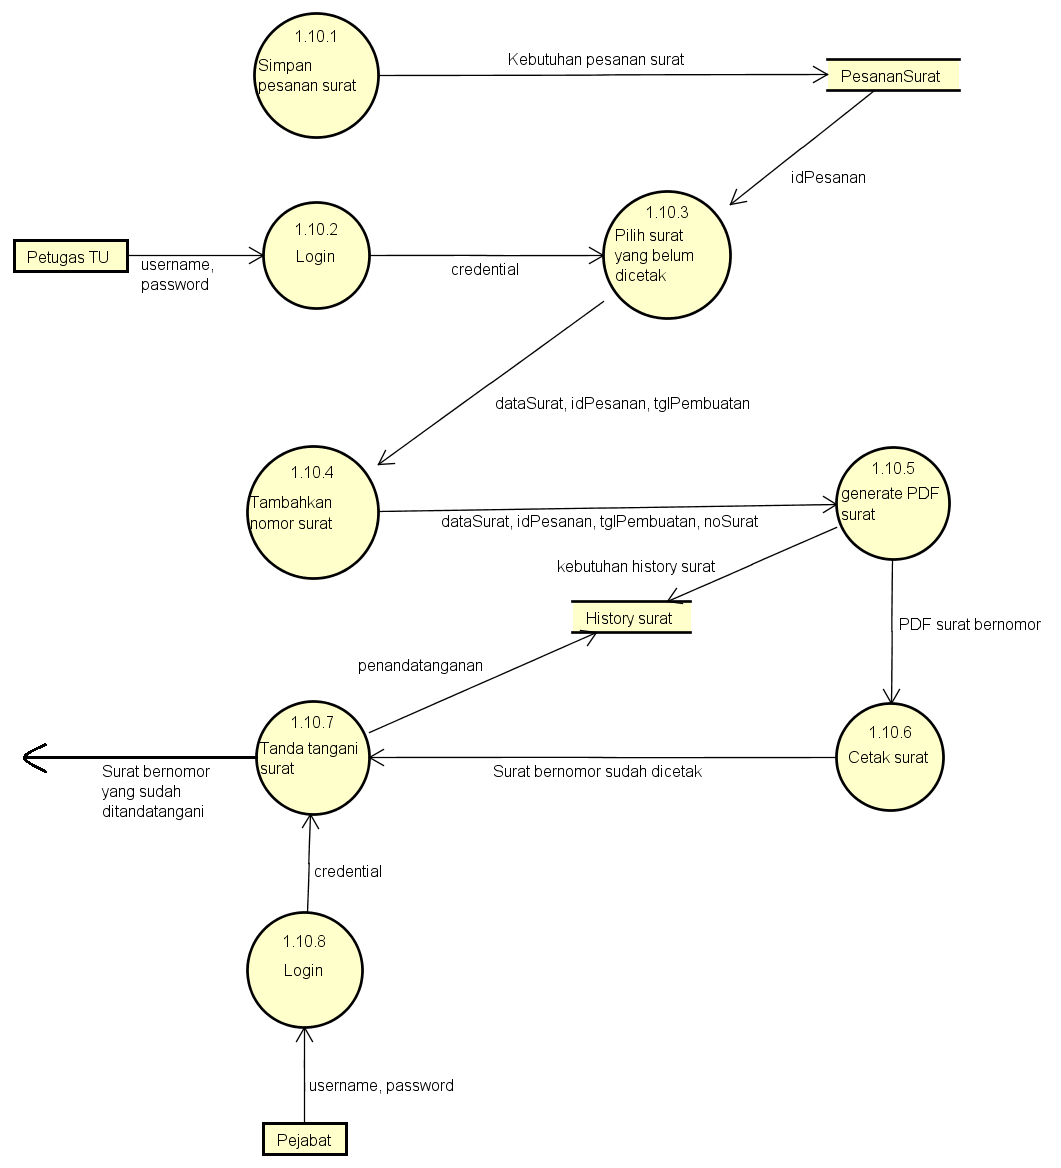
\includegraphics[scale = 0.5]{F:/Skripsi/Dokumentasi_Skripsi/Gambar/Diagram/sistem_usulan/dfd/Lv3-1_10_buat_surat_lanjutan.png}
	\caption{DFD \textit{level} 3-1.10 sebagai lanjutan untuk proses pembuatan surat}
	\label{fig:level_3-1.10}
\end{figure}

Gambar \hyperlink{level_3-1.3}{3.11} merupakan DFD \textit{level} 3-1.3 yang menjelaskan aliran data apabila aktor mahasiswa hendak membuat surat keterangan beasiswa.
\begin{figure}[H]
	\centering
		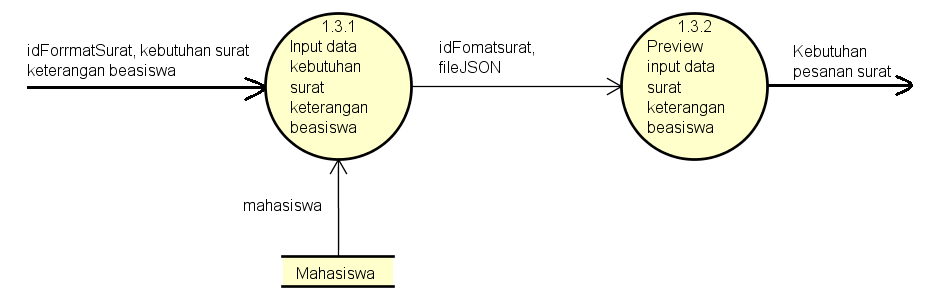
\includegraphics[scale = 0.65]{F:/Skripsi/Dokumentasi_Skripsi/Gambar/Diagram/sistem_usulan/dfd/Lv3-1_3_input_keterangan_beasiswa.png}
	\caption{DFD \textit{level} 3-1.3 untuk pembuatan surat keterangan beasiswa}
	\label{fig:level_3-1.3}
\end{figure}

Gambar \hyperlink{level_3-1.4}{3.12} merupakan DFD \textit{level} 3-1.4 yang menjelaskan aliran data apabila aktor mahasiswa hendak membuat surat keterangan mahasiswa aktif.
\begin{figure}[H]
	\centering
		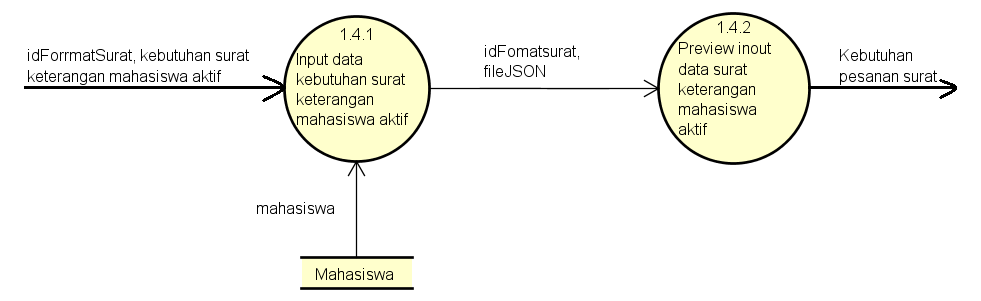
\includegraphics[scale = 0.6]{F:/Skripsi/Dokumentasi_Skripsi/Gambar/Diagram/sistem_usulan/dfd/Lv3-1_4_input_keterangan_mahasiswa_aktif.png}
	\caption{DFD \textit{level} 3-1.4 untuk pembuatan surat keterangan mahasiswa aktif}
	\label{fig:level_3-1.4}
\end{figure}

Gambar \hyperlink{level_3-1.6}{3.13} merupakan DFD \textit{level} 3-1.6 yang menjelaskan aliran data apabila aktor mahasiswa hendak membuat surat pembuatan visa.
\begin{figure}[H]
	\centering
		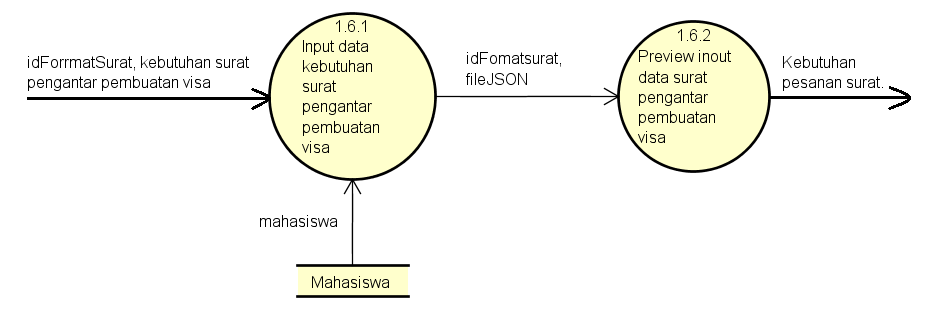
\includegraphics[scale = 0.6]{F:/Skripsi/Dokumentasi_Skripsi/Gambar/Diagram/sistem_usulan/dfd/Lv3-1_6_input_pengantar_pembuatan_visa.png}
	\caption{DFD \textit{level} 3-1.6 untuk pembuatan surat keterangan mahasiswa aktif}
	\label{fig:level_3-1.6}
\end{figure}

Gambar \hyperlink{level_3-1.5}{3.14} merupakan DFD \textit{level} 3-1.5 yang menjelaskan aliran data apabila aktor mahasiswa hendak membuat surat izin studi lapangan.
\begin{figure}[H]
	\centering
		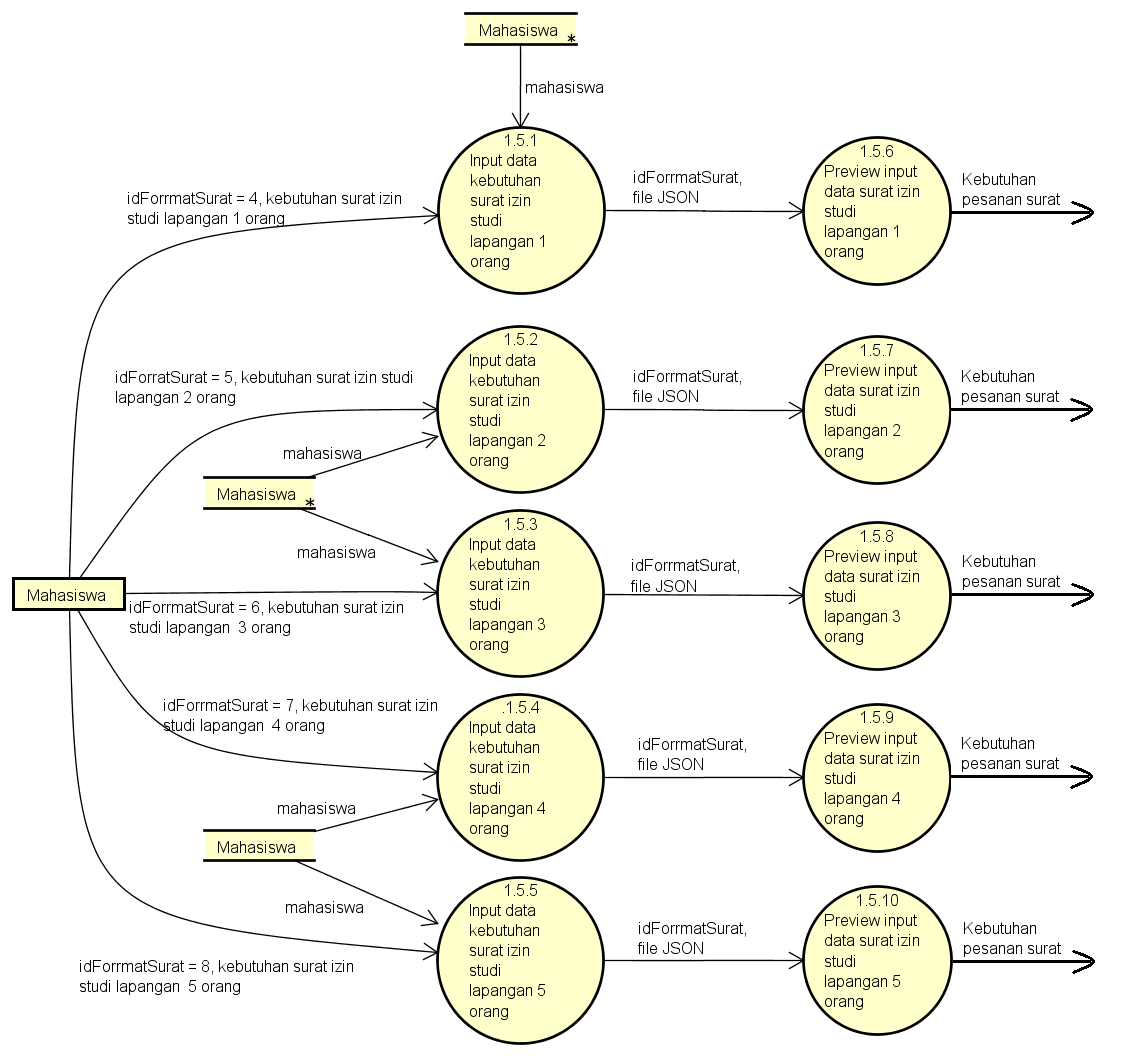
\includegraphics[scale = 0.55]{F:/Skripsi/Dokumentasi_Skripsi/Gambar/Diagram/sistem_usulan/dfd/Lv3-1_5_input_izin_studi_lapangan.png}
	\caption{DFD \textit{level} 3-1.5 untuk pembuatan surat izin studi lapangan}
	\label{fig:level_3-1.5}
\end{figure}

Gambar \hyperlink{level_3-1.7}{3.15} merupakan DFD \textit{level} 3-1.7 yang menjelaskan aliran data apabila aktor mahasiswa hendak membuat surat perwakilan perwalian.
\begin{figure}[H]
	\centering
		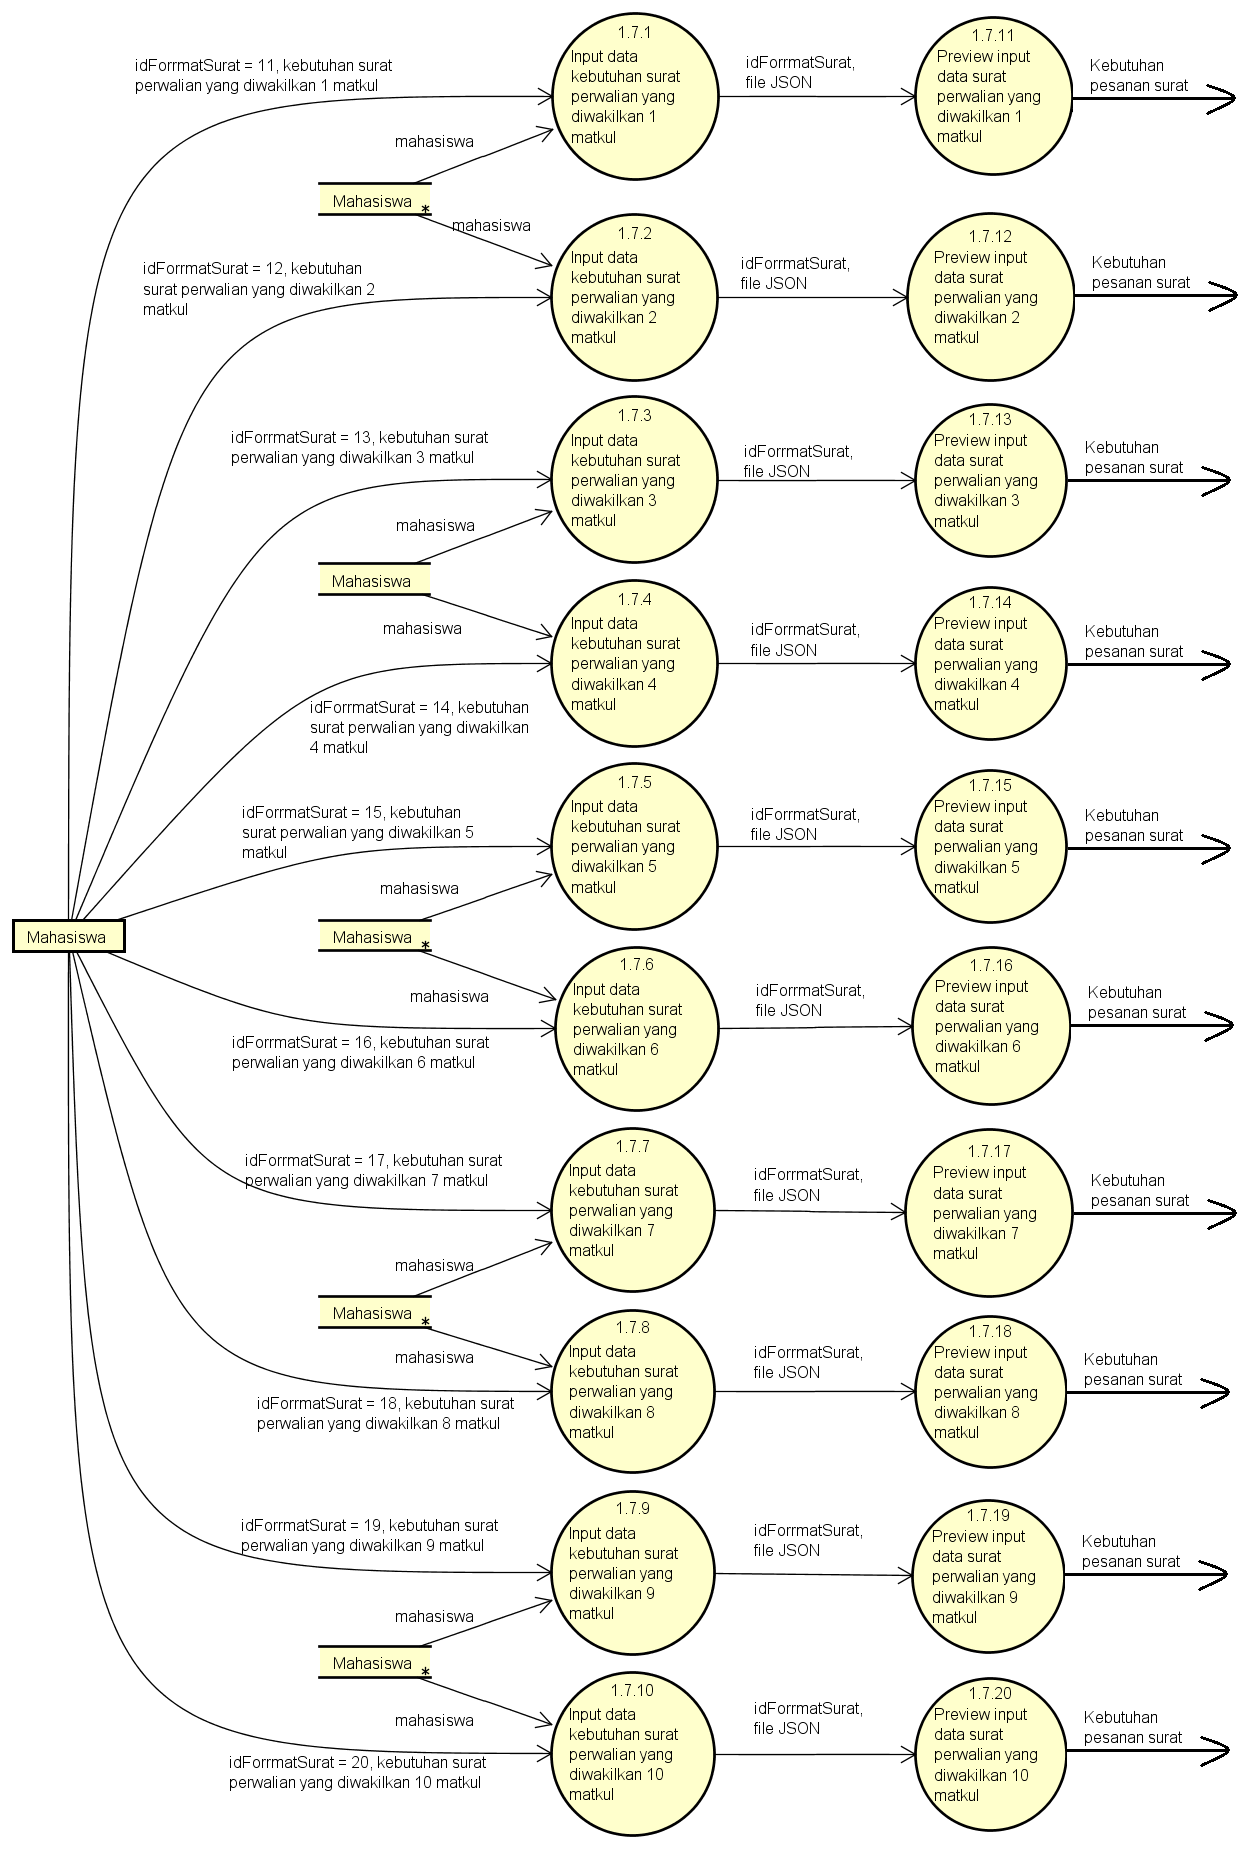
\includegraphics[scale = 0.45]{F:/Skripsi/Dokumentasi_Skripsi/Gambar/Diagram/sistem_usulan/dfd/Lv3-1_7_input_perwakilan_perwalian.png}
	\caption{DFD \textit{level} 3-1.7 untuk pembuatan surat perwakilan perwalian}
	\label{fig:level_3-1.7}
\end{figure}

Gambar \hyperlink{level_3-1.8}{3.16} merupakan DFD \textit{level} 3-1.8 yang menjelaskan aliran data apabila aktor mahasiswa hendak membuat surat izin cuti studi.
\begin{figure}[H]
	\centering
		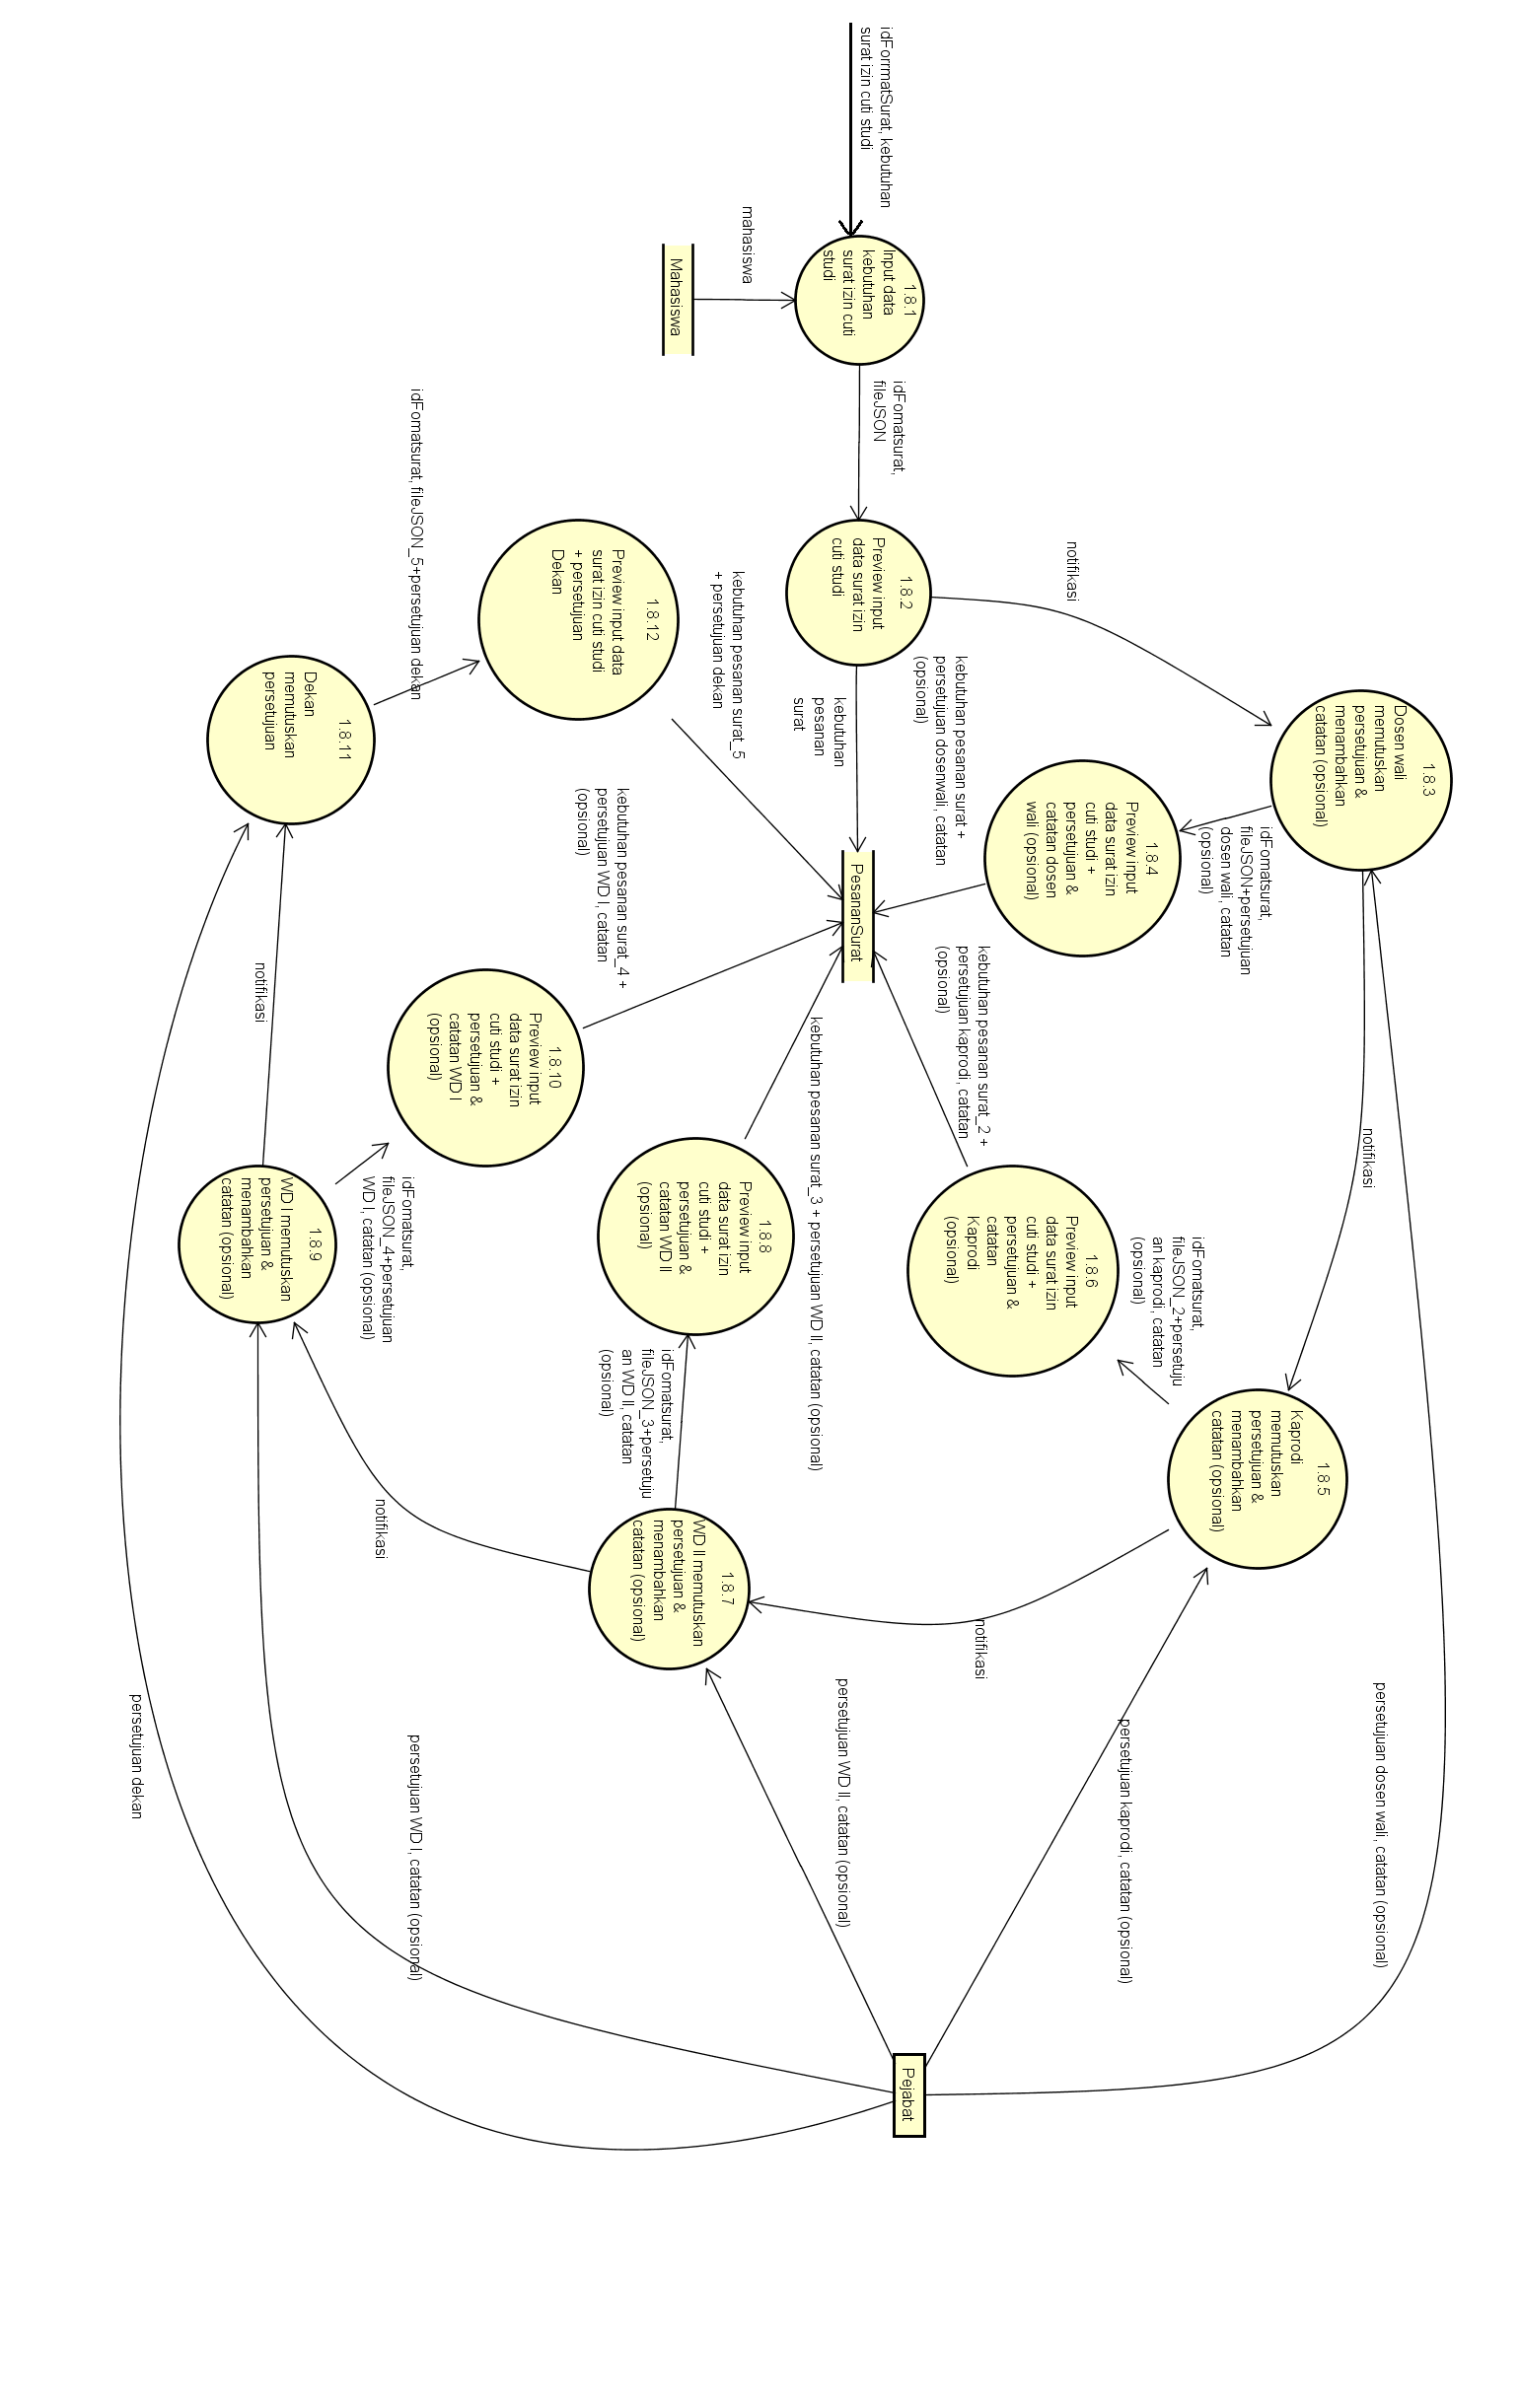
\includegraphics[scale = 0.35]{F:/Skripsi/Dokumentasi_Skripsi/Gambar/Diagram/sistem_usulan/dfd/Lv3-1_8_input_izin_cuti_studi-kiri.png}
	\caption{DFD \textit{level} 3-1.8 untuk pembuatan surat izin cuti studi}
	\label{fig:level_3-1.8}
\end{figure}

Gambar \hyperlink{level_3-1.9}{3.17} merupakan DFD \textit{level} 3-1.9 yang menjelaskan aliran data apabila aktor mahasiswa hendak membuat surat izin pengunduran diri.
\begin{figure}[H]
	\centering
		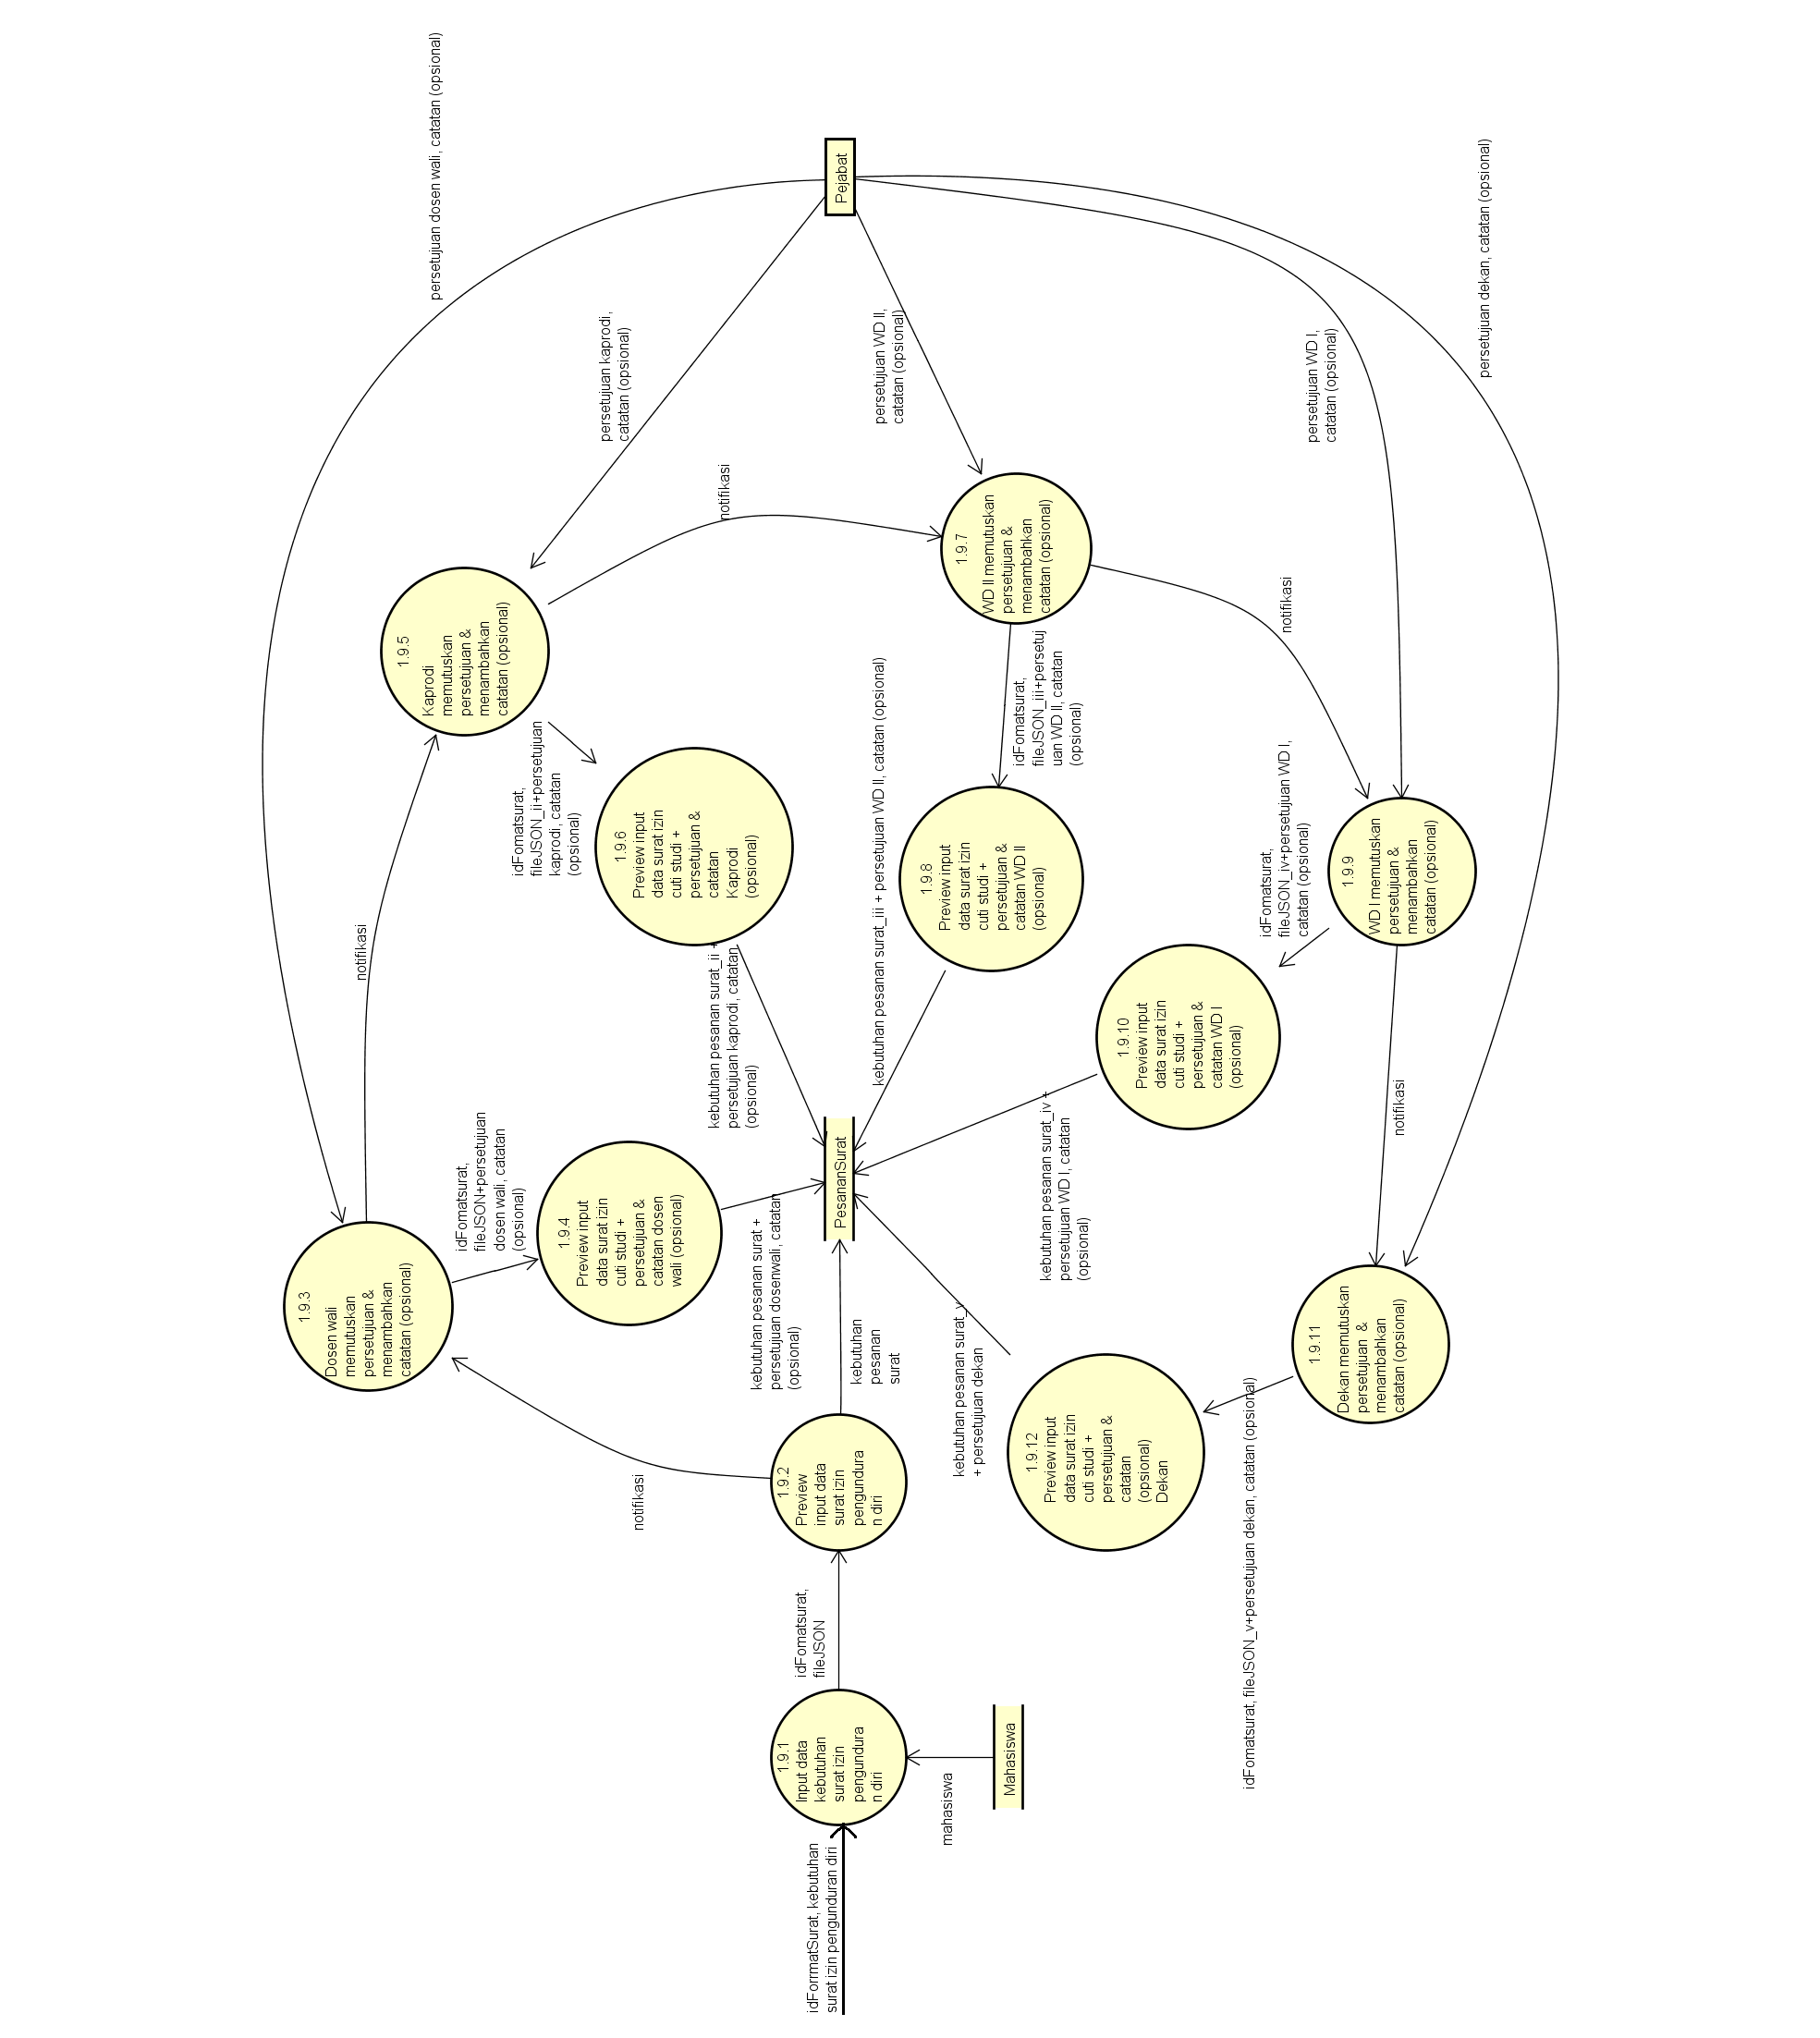
\includegraphics[scale = 0.35]{F:/Skripsi/Dokumentasi_Skripsi/Gambar/Diagram/sistem_usulan/dfd/Lv3-1_9_input_izin_pengunduran_diri-kanan.png}
	\caption{DFD \textit{level} 3-1.9 untuk pembuatan surat izin penguunduran diri}
	\label{fig:level_3-1.9}
\end{figure}

Gambar \hyperlink{level_2-2}{3.18} merupakan DFD \textit{level} 2-2 yang menjelaskan aliran data pada saat aktor mahasiswa hendak mengambil surat.

\begin{figure}[H]
	\centering
		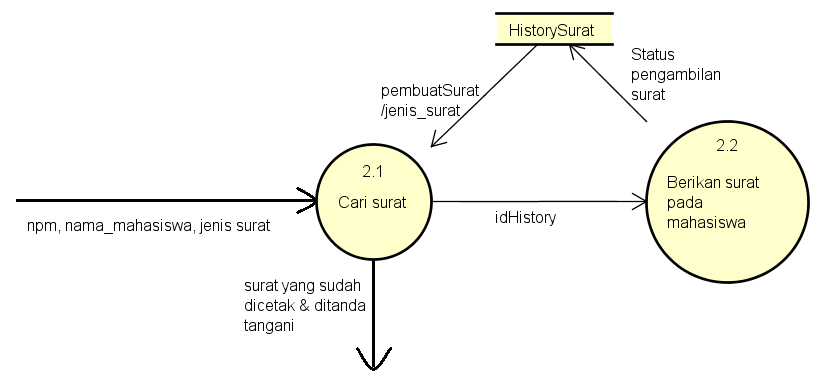
\includegraphics[scale = 0.5]{F:/Skripsi/Dokumentasi_Skripsi/Gambar/Diagram/sistem_usulan/dfd/Lv2-2_pengambilan_surat.png}
	\caption{DFD \textit{level} 2-2 pengambilan surat}
	\label{fig:level_2-2}
\end{figure}

Gambar \hyperlink{level_2-3}{3.19} merupakan DFD \textit{level} 2-3 yang menjelaskan aliran data pada saat aktor petugas TU melakukan operasi CRUD pada \textit{database} format surat.

\begin{figure}[H]
	\centering
		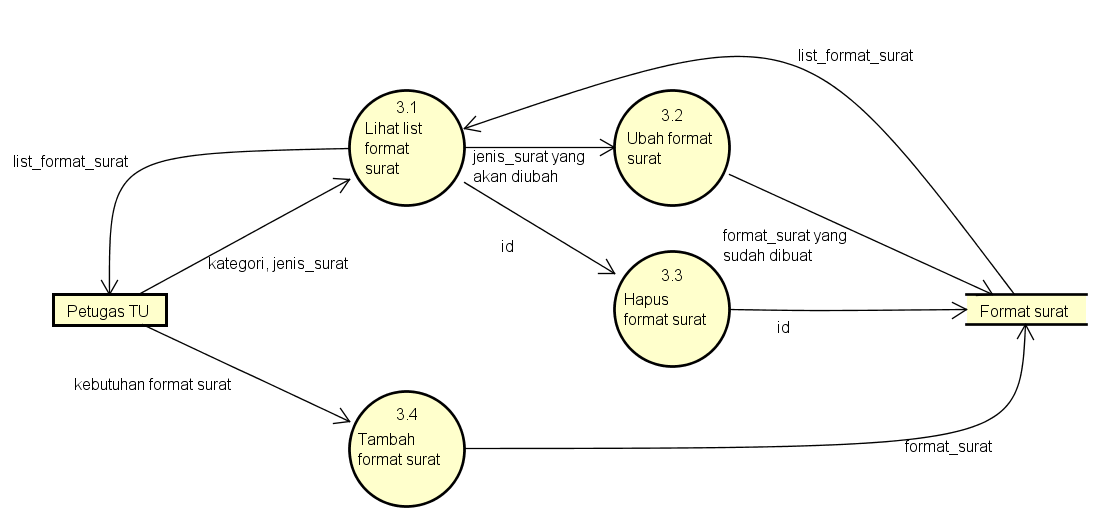
\includegraphics[scale = 0.5]{F:/Skripsi/Dokumentasi_Skripsi/Gambar/Diagram/sistem_usulan/dfd/Lv2-3_kelola_format_surat.png}
	\caption{DFD \textit{level} 2-3 operasi CRUD pada \textit{database} format surat}
	\label{fig:level_2-3}
\end{figure}

Gambar \hyperlink{level_2-4}{3.20} merupakan DFD \textit{level} 2-4 yang menjelaskan aliran data pada saat aktor petugas TU melakukan operasi CRUD pada \textit{database} data mahasiswa.

\begin{figure}[H]
	\centering
		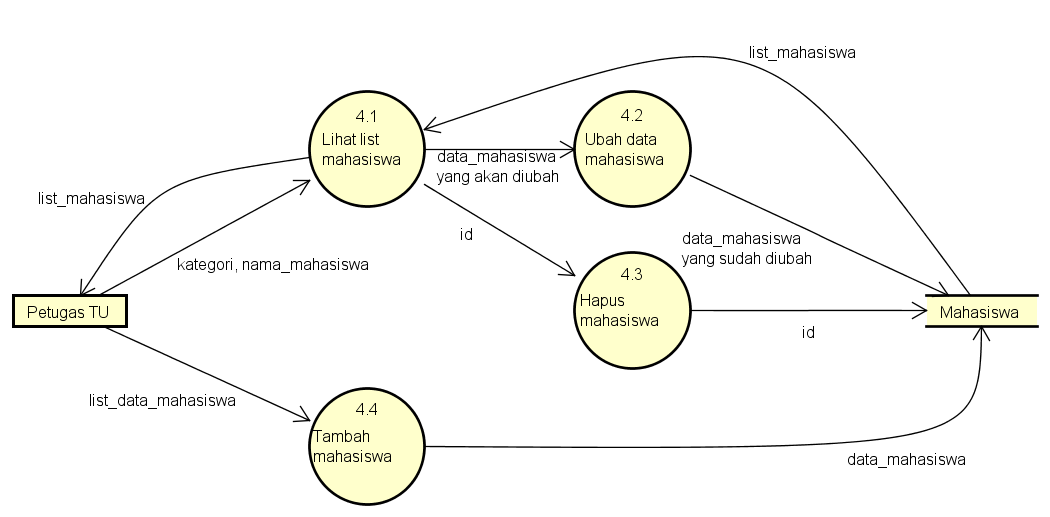
\includegraphics[scale = 0.5]{F:/Skripsi/Dokumentasi_Skripsi/Gambar/Diagram/sistem_usulan/dfd/Lv2-4_kelola_data_mahasiswa.png}
	\caption{DFD \textit{level} 2-4 operasi CRUD pada \textit{database} data mahasiswa}
	\label{fig:level_2-4}
\end{figure}


\subsection{Analisis Kebutuhan Data}
\label{sec:analisis_kebutuhan_data}
Setiap surat memiliki kebutuhan data yang berbeda-beda bergantung dari jenis surat yang akan dibuat. Tabel 3.16-3.20 berikut ini akan menjelaskan data apa saja yang perlu diisikan oleh mahasiswa dalam proses pembuatan surat akademik.\
\begin{table}[H]
\centering
\caption{Tabel Kebutuhan Data Surat Perwakilan Perwalian}
\label{surat_perwakilan_perwalian}
\begin{tabular}{|l|}
\hline
\textbf{Atribut Data}                     \\ \hline
Semester            											\\ \hline
Tahun akademik								            \\ \hline
Nama mahasiswa yang diwakilkan            \\ \hline 
NPM mahasiswa yang diwakilkan             \\ \hline 
Program Studi mahasiswa yang diwakilkan   \\ \hline 
Nama mahasiswa yang diberi kuasa          \\ \hline 
NPM mahasiswa yang diberi kuasa           \\ \hline 
Program studi mahasiswa yang diberi kuasa \\ \hline 
Alasan tidak hadir perwalian               \\ \hline 
Mata kuliah yang diambil                  \\ \hline 
Tanggal pembuatan surat                   \\ \hline
Nama dosen wali								            \\ \hline
Nama wakil dekan I								        \\ \hline
\end{tabular}
\end{table}
\
\begin{table}[H]
\centering
\caption{Tabel Kebutuhan Data Surat Izin Pengunduran Diri}
\label{surat_izin_pengunduran_diri}
\begin{tabular}{|l|}
\hline
{\textbf{Atribut Data}}                     \\ \hline
{Nama mahasiswa}                            \\ \hline 
{NPM}                                       \\ \hline 
{NIRM}                                      \\ \hline 
{Alamat (tetap/di Badung)}                  \\ \hline 
{Nomor telepon (HP)}                        \\ \hline 
{Nama orang tua}                            \\ \hline 
{Tanggal surat}                             \\ \hline 
{Semester berhenti}                         \\ \hline 
{Catatan Dosen Wali}                        \\ \hline 
{Catatan Ketua Program Studi}               \\ \hline 
{Catatan Wakil Dekan I}                     \\ \hline 
{Catatan Wakil Dekan II}                    \\ \hline 
{Catatan Dekan}                             \\ \hline
\end{tabular}
\end{table}
\
\begin{table}[H]
\centering
\caption{Tabel Kebutuhan Data Surat Keterangan}
\label{surat_keterangan}
\begin{tabular}{|l|}
\hline
{\textbf{Atribut Data}}                     \\ \hline
{Nama mahasiswa}                            \\ \hline 
{NPM}                                       \\ \hline 
{Program studi}                             \\ \hline 
{Tempat, tanggal lahir}                     \\ \hline 
{Alamat di Bandung}                         \\ \hline 
{E-mail (selain e-mail Unpar)}               \\ \hline 
{Jenis surat yang akan dibuat}              \\ \hline 
{Alasan pembuatan surat}                    \\ \hline 
{Tahun akademik}                            \\ \hline 
{Nomor telepon (HP)}                        \\ \hline

\end{tabular}
\end{table}
\
\begin{table}[H]
\centering
\caption{Tabel Kebutuhan Data Surat Keterangan Beasiswa}
\label{surat_keterangan_beasiswa}
\begin{tabular}{|l|}
\hline
{\textbf{Atribut Data}}                     \\ \hline
{Nama mahasiswa}                            \\ \hline 
{NPM}                                       \\ \hline 
{Program studi}                             \\ \hline
{Nomor HP}			                            \\ \hline
{Alamat}        			                     	\\ \hline
{Jenis beasiswa}                            \\ \hline 
{Tanggal}                                   \\ \hline 
{Nama orang tua}                            \\ \hline
\end{tabular}
\end{table}
\
\begin{table}[H]
\centering
\caption{Tabel Kebutuhan Data Surat Izin Cuti Studi}
\label{surat_izin_cuti_studi}
\begin{tabular}{|l|}
\hline
{\textbf{Atribut Data}}                     \\ \hline
{Nama mahasiswa}                            \\ \hline 
{NPM}                                       \\ \hline 
{Fakultas}                                  \\ \hline 
{Program studi}                             \\ \hline 
{Alamat tetap}                              \\ \hline
{Cuti studi ke-n}   			                	\\ \hline 
{Alasan cuti studi ke-n}                    \\ \hline
{Dosen Wali}				                        \\ \hline 
{Catatan Dosen Wali}                        \\ \hline
{Catatan Ketua Progam Studi}                \\ \hline 
{Rekomendasi Pembantu Dekan II}             \\ \hline 
{Rekomendasi Pembantu Dekan I}              \\ \hline 
{Semester}                          		    \\ \hline 
{Tahun akademik}                            \\ \hline
{Persetujuan Dekan}                         \\ \hline 
{Tanggal surat}                             \\ \hline
\end{tabular}
\end{table}
}{}
\ifdefstring{\vbabd}{1}{\chapter{Perancangan}
\label{chap:perancangan}

\section{Struktur Modul}
\label{sec:struktur_modul}
Berdasarkan fitur-fitur yang ada pada \textit{website} penyedia surat akademik, maka dirancang struktur modul yang menjelaskan mengenai modul-modul apa saja yang akan dirancang untuk membangun website penyedia surat akademik. Garis besar dari struktur modul ini terbagi menjadi 3 bagian berdasarkan penggunanya, yaitu modul mahasiswa, modul TU dan modul pejabat.\
Gambar \hyperlink{struktur_modul_garis_besar}{4.1} menjelaskan struktur modul secara garis besar.



Selanjutnya, modul-modul yang telah disebutkan sebelumnya memiliki struktur tersendiri yang lebih spesifik. Gambar \hyperlink{struktur_modul_mahasiswa}{4.2} menjelaskan struktur modul mahasiswa secara menyeluruh.



Berdasarkan gambar di atas, berikut ini adalah penjelasan mengenai struktur modul mahasiswa dari \textit{website} penyedia surat akademik :
\begin{enumerate}
	\item Modul \textit{login}.
	\item Modul buat surat.
	\item Modul cek riwayat pembuatan surat.
\end{enumerate}

Gambar \hyperlink{struktur_modul_tu}{4.3} menjelaskan struktur modul TU secara menyeluruh.

%\begin{figure}[H]
%	\centering
%		\includegraphics{}
%		\caption{Struktur modul TU}
%		\label{fig:struktur_modul_tu}
%\end{figure}

Berdasarkan gambar di atas, berikut ini adalah penjelasan mengenai struktur modul TU dari \textit{website} penyedia surat akademik :
\begin{enumerate}
	\item Modul \textit{login}.
	\item Modul data mahasiswa.
	\item Modul format surat.
	\item Modul cek riwayat seluruh pembuatan surat.
\end{enumerate}

Gambar \hyperlink{struktur_modul_pejabat}{4.4} menjelaskan struktur modul pejabat secara menyeluruh.

%\begin{figure}[h]
%	\centering
%		\includegraphics{}
%		\caption{Struktur modul pejabat}
%		\label{fig:struktur_modul_pejabat}
%\end{figure}

Berdasarkan gambar di atas, berikut ini adalah penjelasan mengenai struktur modul pejabat dari \textit{website} penyedia surat akademik :
\begin{enumerate}
	\item Modul \textit{login}.
	\item Modul cek riwayat seluruh pembuatan surat.
\end{enumerate}

\iffalse
\section{Perancangan Antar Muka}
\label{sec:perancangan_antar_muka}

\section{Perancangan Fisik Basis Data}
\label{sec:perancangan_fisik_basis_data}
\fi}{}  
\ifdefstring{\vbabe}{1}{\chapter{Implementasi dan Pengujian}
\label{chap:implementasi_dan_pengujian}

\section{Lingkungan Implementasi}
\label{sec:lingkungan_implementasi}

\subsection{Lingkungan Perangkat Keras}
\label{sec:lingkungan_perangkat_keras}
Untuk membangun website penyedia surat akademik, spesifikasi perangkat keras yang digunakan sebagai berikut :
\begin{itemize}
	\item Processor : Intel(R) Core(TM)i7-4702MQ CPU @2.20GHz
	\item Memory : DDR3 4 GB
	\item Harddisk : 1 TB
	\item VGA :
	\item Monitor
	\item Keyboard dan Mouse
\end{itemize}

\subsection{Lingkungan Perangkat Lunak}
\label{sec:lingkungan_perangkat_lunak}
Untuk membangun website penyedia surat akademik, spesifikasi perangkat lunak yang digunakan sebagai berikut :
\begin{itemize}
	\item Web server : 
	\item Tools : 
	\item Bahasa pemrograman: 
	\item Database management system :
	\item Operation system : 
	\item Keyboard dan Mouse
\end{itemize}}{}
\ifdefstring{\vbabf}{1}{\chapter{Kesimpulan dan Saran}
\label{chap:kesimpulan_dan_saran}

Pada bab ini berisi kesimpulan yang didapat setelah melakukan pembangunan \textit{website} SIKSA serta saran-saran yang dapat digunakan untuk pengembangan penelitian selanjutnya.

\section{Kesimpulan}
\label{sec:kesimpulan}
Setelah melakukan pembangunan \textit{website} SIKSA dapat ditarik beberapa kesimpulan dalam penelitian ini, yaitu :
\begin{enumerate}
	\item Telah berhasil mengidentifikasikan semua surat akademik bersama dengan kebutuhannya. Pada saat dilakukan survei didapat ada 10 surat akademik yang disediakan oleh bagian TU FTIS. Namun karena tidak semua surat tersebut menghasilkan surat yang kemudian akan dikembalikan kepada mahasiswa yang bersangkutan untuk kemudian disampaikan kepada lembaga yang membutuhkan surat tersebut. Maka didapat 6 surat yang kemudian menjadi 7 surat karena adanya surat dengan fungsi ganda.
	\item Telah berhasil mengidentifikasi dan mempelajari setiap \textit{template} surat akademik yang disediakan oleh bagian TU FTIS dan mengimplementasikan setiap \textit{template} surat akademik tersebut ke dalam format \LaTeX. Untuk beberapa format surat ada yang memiliki lebih dari 1 \textit{template} surat akademik dikarenakan ada beberapa perbedaan pada \textit{input}.
	\item Telah berhasil mengimplementasikan pembuatan surat akademik secara otomatis berdasarkan \textit{template} yang telah ditentukan. \textit{Website} yang telah dibangun mengimplementasikan konsep \textit{mailmerge} pada \LaTeX.
	\item Membangun \textit{website} yang dapat memproduksi surat akademik menggunakan \textit{framework} Laravel dan \textit{css bootstrap}. \textit{Website} yang dibangun mengadaptasi formulir isian yang sebelumnya telah digunakan sehingga tidak akan mempersulit bagi pengguna apabila hendak melakukan pemesanan surat.

\end{enumerate}

\section{Saran}
\label{sec:saran}
\textit{Website} SIKSA yang dibangun ini masih dapat dikembangkan lagi. Berdasarkan analisis \textit{website} yang dirancang, ada beberapa saran yang dapat diberikan untuk mengembangkan sistem ini, yaitu:
\begin{enumerate}
	\item Menambahkan fitur \textit{upload} data mahasiswa untuk menambahkan mahasiswa ke \textit{database}.
	\item Menambahkan foto dosen dan petugas TU pada bagian profil pengguna.
\end{enumerate}}{}
\ifdefstring{\vbabg}{1}{\include{Bab/bab7}}{}
\ifdefstring{\vbabh}{1}{\include{Bab/bab8}}{}
\ifdefstring{\vbabi}{1}{\include{Bab/bab9}}{}

\bibliographystyle{compj} 
\bibliography{referensi}

\appendix
%\apptoc 
 
\tampillmp{\vlmp}
\ifdefstring{\vlmpa}{1}{%versi 2 (8-10-2016)
\chapter{Kode Program \textit{View}}
\label{lamp:A}

%selalu gunakan single spacing untuk source code !!!!!
\singlespacing 
% language: bahasa dari kode program
% terdapat beberapa pilihan : Java, C, C++, PHP, Matlab, R, dll
%
% basicstyle : ukuran font untuk kode program
% terdapat beberapa pilihan : tiny, scriptsize, footnotesize, dll
%
% caption : nama yang akan ditampilkan di dokumen akhir, lihat contoh

\begin{lstlisting}[language=php, basicstyle=\tiny, caption=\textit{Home} mahasiswa]
	<!DOCTYPE html>
  <head>
      <title>Home - Mahasiswa</title>
      <link href="{{ asset("/bootstrap-3.3.7-dist/css/bootstrap.css") }}" rel="stylesheet" type="text/css" />
      <link href="{{ asset("/css/styles_list_surat.css") }}" rel="stylesheet" type="text/css">

  </head>

  <body>
    <div>
        <img id=banner src="{{ asset("/images/banner ftis.png") }}" />
    </div>

    <!-- Navigation here -->
    @include('mahasiswa.menu')

    <div class="container">
      <div class="main">
          <div class="row">
            <div class="col-md-8 content">
              <form class="form-inline" action= "{{ url('/data_mahasiswa') }}" method="get">
                <div class="form-group">
                  <label for="kategori_mahasiswa">Cari berdasarkan :</label><br>
                  <select name="kategori" class="form-control">
                    <option value="tanggalBuat">Cari semua surat</option>
                    <option value="tanggalBuat">Tanggal pembuatan</option>
                    <option value="perihal">Perihal</option>
                    <option value="kepada">Kepada</option>
                    <option value="jenis_surat">Jenis surat</option>
                  </select>
                </div>
                <div class="form-group">
                  <label for="searchBox">Kata kunci :</label><br>
                  <input type="text" name="searchBox" class="form-control" size="80" />
                  <button type="submit" name="findmail" class="btn btn-primary">Cari surat</button>
                </div>
              </form>
              <br>
              <table class="table table-striped">
                @if($historysurats != null)
                  @if(count($historysurats) == 0)
                      <tr>
                          <td colspan="5" align="center">Tidak ada history surat....</td>
                      </tr>
                  @else
                      <tr>
                        <th>TANGGAL PEMBUATAN</th>
                        <th>PERIHAL</th>
                        <th>KEPADA</th>
                        <th>JENIS SURAT</th>
                      </tr>
                      @foreach($historysurats as $historysurat)
                        <tr>
                          <td class="ctr">{{ $historysurat->created_at }}</td>
                          <td class="ctr">{{ $historysurat->perihal }}</td>
                          <td class="ctr">{{ $historysurat->penerimaSurat }}</td>
                          <td class="ctr">{{ $historysurat->formatsurat->jenis_surat }}</td>
                        </tr>
                      @endforeach
                  @endif
                @endif
              </table>
            </div>
            @include('mahasiswa.profile_bar')
          </div>
      </div>
    </div>
    <div class="footer">
    </div>
  </body>
</html>

\end{lstlisting}


\begin{lstlisting}[language=Java,basicstyle=\tiny,caption=Pilih kategori surat]
	
<!DOCTYPE html>
  <head>
      <title>Home</title>
      <link href="{{ asset("/bootstrap-3.3.7-dist/css/bootstrap.css") }}" rel="stylesheet" type="text/css" />
      <link href="{{ asset("/css/styles_list_surat.css") }}" rel="stylesheet" type="text/css">

  </head>

  <body>
    <div>
        <img id=banner src="{{ asset("/images/banner ftis.png") }}" />
    </div>


    <!-- Navigation Here -->
    @include('mahasiswa.menu')

    <div class="container">
      <div class="main">
        <div class="row">
          <div class="col-md-8 content">
            <h1>Pilih Kategori Surat</h1>
            <br>
            <form class="form-horizontal" action="{{ url('/pilih_jenis_surat') }}" method="post">
              <div class="form-group">
                <div class="col-sm-9">
                    <div class="radio">
                      <label>
                        <input type="radio"  name="jenis_surat" value="surat_izin" required>
                        Surat Izin
                      </label>
                    </div>
                    <div class="radio">
                      <label>
                        <input type="radio"  name="jenis_surat" value="surat_keterangan" required>
                        Surat Keterangan
                      </label>
                    </div>
                    <div class="radio">
                      <label>
                        <input type="radio"  name="jenis_surat" value="surat_perwakilan" required>
                        Surat Perwakilan
                      </label>
                    </div>
                    <div class="radio">
                      <label>
                        <input type="radio"  name="jenis_surat" value="surat_pengantar" required>
                        Surat Pengantar
                      </label>
                    </div>
                </div>
              </div>
              {!! csrf_field() !!}
              <div class="form-group">
                <div class="col-sm-6">
                  <button type="submit" class="btn btn-primary">Lanjutkan</button>
                </div>
              </div>
            </form>
          </div>
          @include('mahasiswa.profile_bar')
        </div>
      </div>
    </div>
    <div class="footer">
    </div>
  </body>
</html>

\end{lstlisting}

\begin{lstlisting}[language=Java,basicstyle=\tiny,caption=Pilih jenis surat keterangan]
	<!DOCTYPE html>
  <head>
      <title>Pilih Jenis Surat</title>
      <link href="{{ asset("/bootstrap-3.3.7-dist/css/bootstrap.css") }}" rel="stylesheet" type="text/css" />
      <link href="{{ asset("/css/styles_list_surat.css") }}" rel="stylesheet" type="text/css">

  </head>

  <body>
    <div>
        <img id=banner src="{{ asset("/images/banner ftis.png") }}" />
    </div>


    <!-- Navigation Here -->
    @include('mahasiswa.menu')

    <div class="container">
      <div class="main">
        <div class="row">
          <div class="col-md-8 content">
            <h1>Pilih Jenis Surat</h1>
            <br>
            <form class="form-horizontal" action="{{ url('/isi_data_diri') }}" method="post">
              <div class="form-group">
                <div class="col-sm-9">
                    @foreach($formatsurats as $formatsurat)
                      @if(($formatsurat->id == 1) || ($formatsurat->id == 2))
                        <div class="radio">
                          <label>
                            <input type="radio"  name="jenis_surat" value="{{ $formatsurat->id }}" required>
                            {{ $formatsurat->jenis_surat }}
                          </label>
                        </div>
                      @endif
                    @endforeach
                </div>
              </div>
              {!! csrf_field() !!}
              <div class="form-group">
                <div class="col-sm-6">
                  <button type="submit" class="btn btn-primary">Lanjutkan</button>
                </div>
              </div>
            </form>
          </div>
          @include('mahasiswa.profile_bar')
        </div>
      </div>
    </div>
    <div class="footer">
    </div>
  </body>
</html>

\end{lstlisting}

\begin{lstlisting}[language=Java,basicstyle=\tiny,caption=Pengisian data keterangan beasiswa.blade.php]
	<!DOCTYPE html>
  <head>
      <title>Isi Data Diri</title>
      <link href="{{ asset("/bootstrap-3.3.7-dist/css/bootstrap.css") }}" rel="stylesheet" type="text/css" />
      <link href="{{ asset("/css/styles_list_surat.css") }}" rel="stylesheet" type="text/css">

  </head>

  <body>
    <div>
        <img id=banner src="{{ asset("/images/banner ftis.png") }}" />
    </div>


    <!-- Navigation here -->
    @include('mahasiswa.menu')

    <div class="container">
      <div class="main">
          <div class="row">
            <div class="col-md-8 content">
              <h1>Isi Data Diri Anda</h1>
              <br>
              <form action = "{{ url('/preview') }}" method="post" class="form-horizontal">
                <div class="form-group">
                  <label for="nama" class="col-sm-3">Nama</label>
                  <div class="col-sm-9">
                    <input type="text" class="form-control" id="nama" name="nama" value="{{ $user->nama_mahasiswa }}" readonly style="border: none" />
                  </div>
                </div>
                <div class="form-group">
                  <label for="prodi" class="col-sm-3">Program studi</label>
                  <div class="col-sm-9">
                    <span type="text" class="form-control" readonly style="border: none" >{{ $user->jurusan->nama_jurusan }}</span>
                    <input type="hidden" name="prodi" value="{{ $user->jurusan_id }}"/>
                  </div>
                </div>
                <div class="form-group">
                  <label for="npm" class="col-sm-3">NPM</label>
                  <div class="col-sm-9">
                    <input type="text" class="form-control" id="npm" name="npm" value="{{ $user->npm }}" readonly style="border: none">
                  </div>
                </div>
                <div class="form-group">
                  <label for="semester" class="col-sm-3">Semester</label>
                  <div class="col-sm-9">
                    <input type="text" class="form-control" name="semester" value="{{ $user->semester }}" readonly style="border: none" />
                  </div>
                </div>
                <div class="form-group">
                  <label for="thnAkademik" class="col-sm-3">Tahun akademik</label>
                  <div class="col-sm-9">
                    <input type="text" class="form-control" name="thnAkademik" value="{{ $user->thnAkademik }}" readonly style="border: none" />
                  </div>
                </div>
                <div class="form-group">
                  <label for="penyediabeasiswa" class="col-sm-3">Penyedia beasiswa</label>
                  <div class="col-sm-9">
                    <input type="text" class="form-control" id="penyediabeasiswa" required name="penyediabeasiswa" >
                  </div>
                </div>
                <input type="hidden" value="{{ $formatsurat_id }}" name="jenis_surat">
                {!! csrf_field() !!}
                <div class="form-group">
                  <div class="col-sm-offset-3 col-sm-10">
                    <button type="submit" class="btn btn-primary">Lanjutkan</button>
                  </div>
                </div>
              </form>
            </div>
            @include('mahasiswa.profile_bar')
          </div>
      </div>
    </div>
    <div class="footer">
    </div>
  </body>
</html>

\end{lstlisting}

\begin{lstlisting}[language=Java,basicstyle=\tiny,caption=Preview isi data keterangan beasiswa]
	<!DOCTYPE html>
  <head>
      <title>Preview</title>
      <link href="{{ asset("/bootstrap-3.3.7-dist/css/bootstrap.css") }}" rel="stylesheet" type="text/css" />
      <link href="{{ asset("/css/styles_list_surat.css") }}" rel="stylesheet" type="text/css">

  </head>

  <body>
    <div>
        <img id=banner src="{{ asset("/images/banner ftis.png") }}" />
    </div>


    <!-- Navigation here -->
    @include('mahasiswa.menu')

    <div class="container">
      <div class="main">
          <div class="row">
            <div class="col-md-8 contentPreview form-horizontal">
              <h4 style="font-weight:bold">SURAT PERNYATAAN</h4>
              <br>

                <form action = "{{ url('/kirimFormulir') }}" method="post">
                  <div class="form-group">
                    <label class="col-sm-3 prevLabel">Nama</label>
                    <div class="col-sm-9" name="nama">
                        {{ $nama }}
                    </div>
                  </div>
                  <div class="form-group">
                    <label class="col-sm-3 prevLabel">Program Studi</label>
                    <div class="col-sm-9" name="prodi">
                      <span>{{ $user->jurusan->nama_jurusan }}</span>
                      <input type="hidden" name="prodi" value="{{ $prodi }}"/>
                    </div>
                  </div>
                  <div class="form-group">
                    <label class="col-sm-3 prevLabel">NPM</label>
                    <div class="col-sm-9" name="npm">
                        {{ $npm }}
                    </div>
                  </div>
                  <div class="form-group">
                    <label class="col-sm-3 prevLabel">Semester</label>
                    <div class="col-sm-9" name="semester">
                        {{ $semester }}
                    </div>
                  </div>
                  <div class="form-group">
                    <label class="col-sm-3 prevLabel">Tahun Akademik</label>
                    <div class="col-sm-9" name="thnAkademik">
                        {{ $thnAkademik }}
                    </div>
                  </div>
                  <div class="form-group">
                    <label class="col-sm-3 prevLabel">Penyedia Beasiswa</label>
                    <div class="col-sm-9" name="penyediabeasiswa">
                        {{ $penyediabeasiswa }}
                    </div>
                  </div>
                  <input type="hidden" value="{{ $formatsurat_id }}" name="idFormat">
                  <input type="hidden" value="{{ $dataSurat }}" name="dataSurat">
                  <input type="hidden" value="{{ $penyediabeasiswa }}" name="provider">
                  {!! csrf_field() !!}
                  <br>
                  <div class="form-group">
                    <div class="col-sm-offset-3 col-sm-10">
                      <button class="btn btn-default" onclick="goBack()">Kembali</button>
                      <button type="submit" class="btn btn-success">Buat Surat</button>
                    </div>
                  </div>
                </form>
            </div>
            @include('mahasiswa.profile_bar')
          </div>
      </div>
    </div>
    <div class="footer">
    </div>
    <script>
      function goBack() {
          window.history.back();
      }
    </script>
  </body>
</html>

\end{lstlisting}

\begin{lstlisting}[language=Java,basicstyle=\tiny,caption=\textit{Navigation bar} untuk mahasiswa]
	<div class="navigation">
     <div class="navbar text-center">
        <ul class="inline">
           <a href="/home_mahasiswa"><li>Home</li></a>
           <a href="/pilih_kategori_surat"><li>Buat Surat</li></a>
           <a href="{{ url('/logout') }}"
               onclick="event.preventDefault();
                        document.getElementById('logout-form').submit();"><li>
               Logout
           <form id="logout-form" action="{{ url('/logout') }}" method="POST" style="display: none;">
               {{ csrf_field() }}
           </form>
           </li></a>
        </ul>
     </div>
</div>
<br/>
<!-- <div class="row">
  <div class="col-md-offset-1 col-sm-offset-1 col-md-4 col-sm-5">
    <div style="color:white">
        Selamat Datang, {!! Auth::user()->name !!}
    </div>
  </div>
</div> -->
<div class="row">
  <div class="col-md-offset-1 col-sm-offset-1 col-sm-4 col-md-4">

  </div>
</div>

\end{lstlisting}

\begin{lstlisting}[language=Java,basicstyle=\tiny,caption=\textit{Sidebar} untuk mahasiswa]
	<div class="col-md-4 profile">
  <div class="card hovercard">
      <div class="cardheader">

      </div>
      <div class="avatar">
          <img alt="" src="{{ $user->foto_mahasiswa }}" />
      </div>
      <div class="info">
          <div class="title">
              {{ $user->nama_mahasiswa }}
          </div>
          <div class="desc">{{ $user->npm }}</div>
          <div class="desc">{{ $user->jurusan->nama_jurusan }}</div>
      </div>
  </div>
</div>

\end{lstlisting}

\begin{lstlisting}[language=Java,basicstyle=\tiny,caption=\textit{Home} pejabat]
	<!DOCTYPE html>
  <head>
      <title>Home - Pejabat</title>
      <link href="{{ asset("/bootstrap-3.3.7-dist/css/bootstrap.css") }}" rel="stylesheet" type="text/css" />
      <link href="{{ asset("/css/styles_list_surat.css") }}" rel="stylesheet" type="text/css">

  </head>

  <body>
    <div>
        <img id=banner src="{{ asset("/images/banner ftis.png") }}" />
    </div>

    <!-- Navigation Here -->
    @include('pejabat.menu')

    <div class="container">
      <div class="main">
          <div class="row">
            <div class="col-md-8 content">
              <form>
                    <table>
                      <tr>
                        <td><label>Kata kunci :</label></td>
                        <td><label>Cari berdasarkan :</label></td>
                      </tr>

                      <tr>
                        <td class = "search">
                          <select name="kategori" class="form-control">
                            <option value="tanggalBuat">Cari semua surat</option>
                            <option value="noSurat">Nomor surat</option>
                            <option value="tanggalBuat">Tanggal pembuatan</option>
                            <option value="perihal">Perihal</option>
                            <option value="kepada]">Kepada</option>
                            <option value="nama">Pembuat surat</option>
                            <option value="idFormatSurat">Jenis surat</option>
                          </select>
                        </td>
                        <td class = "search">
                          <input type="text" name="searchBox" class="form-control" size="68" />
                        </td>
                        <td>
                          <input type="submit" name="findmail" class="btn btn-primary" value="Cari surat" />
                        </td>
                      </tr>
                    </table>
              </form>
              <br>
              <table class="table table-striped">
                <tr>
                  @if(count($pesanansurats) == 0)
                    <tr>
                        <td colspan="5" align="center">Tidak ada pesanan surat ...</td>
                    </tr>
                @else
                    <tr>
                      <th>JENIS SURAT</th>
                      <th>PERIHAL</th>
                      <th>PEMOHON</th>
                      <th>PENERIMA</th>
                      <th>TANGGAL PEMBUATAN</th>
                      <th>DATA SURAT</th>
                      <th>KONTROL</th>
                    </tr>
                    @foreach($pesanansurats as $pesanansurat)
                        <tr>
                          <td class="ctr">{{ $pesanansurat->formatsurat->jenis_surat }}</td>
                          <td class="ctr">{{ $pesanansurat->perihal }}</td>
                          <td class="ctr">{{ $pesanansurat->mahasiswa->nama_mahasiswa }}</td>
                          <td class="ctr">{{ $pesanansurat->penerimaSurat }}</td>
                          <td class="ctr">{{ $pesanansurat->created_at }}</td>
                          <td class="ctr"><textarea rows="5" cols="30" style="border: none" readonly>{{ $pesanansurat->dataSurat }}</textarea></td>
                          <td class="ctr">
                            @if($pesanansurat->formatsurat->id == 9 || $pesanansurat->formatsurat->id == 10)
                            <form action="/persetujuan" method="post">
                              <input type="hidden" value="{{ $pesanansurat->formatsurat_id }}" name="idFormatSurat">
                              <input type="hidden" value="{{ $pesanansurat->dataSurat }}" name="dataSurat">
                              <input type="hidden" value="{{ $pesanansurat->id }}" name="idPesananSurat">
                              {!! csrf_field() !!}
                              <button type="submit" class="btn btn-default">Tambah<br>Persetujuan</button>
                            </form>
                            @else
                              <!-- <span class="btn btn-default"></span> -->
                            @endif
                          </td>
                        </tr>
                    @endforeach
                  @endif
              </table>
            </div>
              @include('pejabat.profile_bar')
          </div>
      </div>
    </div>
    <div class="footer">
    </div>
  </body>
</html>

\end{lstlisting}

\begin{lstlisting}[language=php,basicstyle=\tiny,caption=Tambah persetujuan dan catatan]
	<!DOCTYPE html>
  <head>
      <title>Isi Catatan Dekan</title>
      <link href="{{ asset("/bootstrap-3.3.7-dist/css/bootstrap.css") }}" rel="stylesheet" type="text/css" />
      <link href="{{ asset("/css/styles_list_surat.css") }}" rel="stylesheet" type="text/css">

  </head>

  <body>
    <div>
        <img id=banner src="{{ asset("/images/banner ftis.png") }}" />
    </div>


    <!-- Navigation Here -->
    @include('pejabat.menu')

    <div class="container">
      <div class="main">
          <div class="row">
            <div class="col-md-8 content">
              <h1>Isi Persetujuan & Catatan</h1>
              <br>
              <form class="form-horizontal" method="post" action="/previewCatatan">
                <div class="form-group">
                  <label for="persetujuan" class="col-sm-3">Persetujuan</label>
                  <div class="col-sm-9">
                    <label class="radio-inline">
                      <input type="radio" name="persetujuan" value="Setuju" checked required>Setuju
                    </label>
                    <label class="radio-inline">
                      <input type="radio" name="persetujuan" value="Tidak setuju">Tidak setuju
                    </label>
                  </div>
                </div>
                <div class="form-group">
                  <label for="catatanDekan" class="col-sm-3">Catatan (Opsional)</label>
                  <div class="col-sm-9">
                    <textarea class="form-control" id="catatan" row="5" name="catatan"></textarea>
                  </div>
                </div>
                {!! csrf_field() !!}
                <input type="hidden" value="{{ $dataSurat }}" name="dataSurat">
                <input type="hidden" value="{{ $formatsurat_id }}" name="formatsurat_id">
                <input type="hidden" value="{{ $idPesananSurat }}" name="idPesananSurat">
                <div class="form-group">
                  <div class="col-sm-offset-3 col-sm-10">
                    <button type="submit" class="btn btn-primary">Lanjutkan</button>
                  </div>
                </div>
              </form>
            </div>
            @include('pejabat.profile_bar')
          </div>
      </div>
    </div>
    <div class="footer">
    </div>
  </body>
</html>

\end{lstlisting}

\begin{lstlisting}[language=php,basicstyle=\tiny,caption=\textit{Preview} isi persetujuan dan catatan]
	<!DOCTYPE html>
  <head>
      <title>Isi data diri</title>
      <link href="{{ asset("/bootstrap-3.3.7-dist/css/bootstrap.css") }}" rel="stylesheet" type="text/css" />
      <link href="{{ asset("/css/styles_list_surat.css") }}" rel="stylesheet" type="text/css">

  </head>

  <body>
    <div>
        <img id=banner src="{{ asset("/images/banner ftis.png") }}" />
    </div>


    <!-- Navigation here -->
    @include('mahasiswa.menu')

    <div class="container">
      <div class="main">
          <div class="row">
            <div class="col-md-8 contentPreview form-horizontal">
              <h4 style="font-weight:bold">FORMULIR PERMOHONAN CUTI STUDI</h4>
              <br>
              <form action = "{{ url('/updateFormulir') }}" method="post">
                <div class="form-group">
                  <label for="nama" class="col-sm-3 prevLabel">Nama</label>
                  <div class="col-sm-9" name="nama">
                    {{ $nama }}
                  </div>
                </div>
                <div class="form-group">
                  <label for="npm" class="col-sm-3 prevLabel">NPM</label>
                  <div class="col-sm-9" name="npm">
                    {{ $npm }}
                  </div>
                </div>
                <div class="form-group">
                  <label for="prodi" class="col-sm-3 prevLabel">Program Studi</label>
                  <div class="col-sm-9" name="prodi">
                    {{ $prodi }}
                  </div>
                </div>
                <div class="form-group">
                  <label for="fakultas" class="col-sm-3 prevLabel">Fakultas</label>
                  <div class="col-sm-9" name="fakultas">
                    {{ $fakultas }}
                  </div>
                </div>
                <div class="form-group">
                  <label for="alamat" class="col-sm-3 prevLabel">Alamat</label>
                  <div class="col-sm-9" name="alamat">
                    {{ $alamat }}
                  </div>
                </div>
                <div class="form-group prev">
                  <label for="alasanCutiStudi" class="col-sm-3 prevLabel">Alasan cuti studi ke </label>
                  <div class="col-sm-9" name="alasanCutiStudi">
                    {{ $cutiStudiKe }}<br>
                    {{ $alasanCutiStudi }}
                  </div>
                </div>
                <div class="form-group prev">
                  <label for="catatanDosenWali" class="col-sm-3 prevLabel">Catatan dosen wali </label>
                  <div class="col-sm-9" name="catatanDosenWali">
                    Nama : {{ $dosenWali }}<br>
                    {{ $persetujuanDosenWali }}<br>
                    {{ $catatanDosenWali }}
                    <input type="hidden" name="dosenWali" value="{{ $persetujuanDosenWali }}|{{ $catatanDosenWali }}" />
                  </div>
                </div>
                <div class="form-group prev">
                  <label for="catatanKaprodi" class="col-sm-3 prevLabel">Catatan Kaprodi </label>
                  <div class="col-sm-9" name="catatanKaprodi">
                    {{ $persetujuanKaprodi }}<br>
                    {{ $catatanKaprodi }}
                    <input type="hidden" name="kaprodi" value="{{ $persetujuanKaprodi }}|{{ $catatanKaprodi }}" />
                  </div>
                </div>
                <div class="form-group prev">
                  <label for="catatanWDII" class="col-sm-3 prevLabel">Catatan WD II</label>
                  <div class="col-sm-9" name="catatanWDII">
                    {{ $persetujuanWDII }}<br>
                    {{ $catatanWDII }}
                    <input type="hidden" name="wd2" value="{{ $persetujuanWDII }}|{{ $catatanWDII }}" />
                  </div>
                </div>
                <div class="form-group prev">
                  <label for="catatanWDI" class="col-sm-3 prevLabel">Catatan WD I</label>
                  <div class="col-sm-9" name="catatanWDI">
                    {{ $persetujuanWDI }}<br>
                    {{ $catatanWDI }}
                    <input type="hidden" name="wd1" value="{{ $persetujuanWDI }}|{{ $catatanWDI }}" />
                  </div>
                </div>
                <div class="form-group prev">
                  <label for="persetujuanDekan" class="col-sm-3 prevLabel">Persetujuan Dekan</label>
                  <div class="col-sm-9" name="persetujuanDekan" >
                    {{ $persetujuanDekan }}
                    <input type="hidden" name="dekan" value="{{ $persetujuanDekan }}" />
                  </div>
                </div>
                <div class="form-group prev">
                  <label for="semester" class="col-sm-3 prevLabel">Semester</label>
                  <div class="col-sm-9" name="semester">
                    {{ $semester }}
                  </div>
                </div>
                <div class="form-group prev">
                  <label for="thnAkademik" class="col-sm-3 prevLabel">Tahun Akademik</label>
                  <div class="col-sm-9" name="thnAkademik">
                    {{ $thnAkademik }}
                  </div>
                </div>
                <input type="hidden" value="{{ $formatsurat_id }}" name="idFormat">
                <input type="hidden" value="{{ $dataSurat }}" name="dataSurat">
                <input type="hidden" name="idPesanansurat" value="{{$idPesanansurat}}">

                {!! csrf_field() !!}
                <br>
                <div class="form-group">
                  <div class="col-sm-offset-3 col-sm-10">
                    <button class="btn btn-default" onclick="goBack()">Kembali</button>
                    <button type="submit" class="btn btn-success">Buat Surat</button>
                  </div>
                </div>
              </form>
            </div>
            @include('mahasiswa.profile_bar')
          </div>
      </div>
    </div>
    <div class="footer">
    </div>
    <script>
      function goBack() {
          window.history.back();
      }
    </script>
  </body>
</html>
	
\end{lstlisting}

\begin{lstlisting}[language=php,basicstyle=\tiny,caption=\textit{History} pejabat]
	<!DOCTYPE html>
  <head>
      <title>Data Mahasiswa</title>
      <link href="{{ asset("/bootstrap-3.3.7-dist/css/bootstrap.css") }}" rel="stylesheet" type="text/css" />
      <link href="{{ asset("/css/styles_list_surat.css") }}" rel="stylesheet" type="text/css">
  </head>

  <body>
    <div>
        <img id=banner src="{{ asset("/images/banner ftis.png") }}" />
    </div>

    <!-- Navigation Here -->
    @include('pejabat.menu')

    <div class="container">
      <div class="main">
          <div class="row">
            <div class="col-md-8 content">
              <form class="form-inline" action= "{{ url('/format_surat') }}" method="get">
                <div class="form-group">
                  <label for="kategori_format_surat">Cari berdasarkan :</label><br>
                  <select name="kategori_mahasiswa" class="form-control">
                    <option value="">Cari semua surat</option>
                    <option value="noSurat">Nomor Surat</option>
                    <option value="jenis_surat">Jenis Surat</option>
                    <option value="perihal">Perihal</option>
                    <option value="pemohon">Pemohon</option>
                    <option value="penerima">Penerima</option>
                    <option value="tanggalPembuatan">Tanggal Pembuatan</option>
                  </select>
                </div>
                <div class="form-group">
                  <label for="searchBox_format_surat">Kata kunci :</label><br>
                  <input type="text" name="searchBox" class="form-control" size="68" />
                  <button type="submit" name="findmail" class="btn btn-primary">Cari surat</button>
                </div>
              </form>
              <br>
              <table class="table table-striped table-hover">
                @if($historysurats != null)
                  @if(count($historysurats) == 0)
                      <tr>
                          <td colspan="5" align="center">Tidak ada history surat....</td>
                      </tr>
                  @else
                      <tr>
                        <th>NOMOR SURAT</th>
                        <th>JENIS SURAT</th>
                        <th>PERIHAL</th>
                        <th>PEMOHON</th>
                        <th>PENERIMA</th>
                        <th>TANGGAL PEMBUATAN</th>
                        <th>PENANDATANGANAN</th>
                        <th>PENGAMBILAN</th>
                      </tr>
                      @foreach($historysurats as $historysurat)
                        <tr>
                          <td class="ctr">{{ $historysurat->no_surat }}</td>
                          <td class="ctr">{{ $historysurat->formatsurat->jenis_surat }}</td>
                          <td class="ctr">{{ $historysurat->perihal }}</td>
                          <td class="ctr">{{ $historysurat->mahasiswa->nama_mahasiswa  }}</td>
                          <td class="ctr">{{ $historysurat->penerimaSurat }}</td>
                          <td class="ctr">{{ $historysurat->created_at }}</td>
                          <td align="center">
                            @if($historysurat->penandatanganan)
                              <button type="submit" disabled class="btn btn-success" style="display:block">Sudah</button>
                            @else
                              <form action="{{url('/ubahStatusPenandatanganan')}}" method="post">
                                <input type="hidden" value="{{ $historysurat->id }}" name="id">
                                {!! csrf_field() !!}
                                <button type="submit" class="btn btn-default " style="display:block">Belum</button>
                              </form>
                            @endif
                          </td>
                          <td class="ctr">
                            @if($historysurat->pengambilan)
                              <p>Sudah</p>
                            @else
                              <p>Belum</p>
                            @endif
                          </td>
                        </tr>
                      @endforeach
                  @endif
                @endif
              </table>
              <div style="text-align:center">{!! $historysurats->links() !!}</div>
            </div>
            @include('pejabat.profile_bar')
          </div>
      </div>
    </div>
    <div class="footer">
    </div>
  </body>
</html>

\end{lstlisting}

\begin{lstlisting}[language=php,basicstyle=\tiny,caption=\textit{Navigation bar} untuk pejabat]
	<div class="navigation">
     <div class="navbar text-center">
        <ul class="inline">
          <a href="/home_pejabat"><li>Home</li></a>
          <a href="/history_pejabat"><li>History Surat</li></a>

          <a href="{{ url('/logout') }}"
              onclick="event.preventDefault();
                       document.getElementById('logout-form').submit();"><li>
              Logout
          <form id="logout-form" action="{{ url('/logout') }}" method="POST" style="display: none;">
              {{ csrf_field() }}
          </form>
          </li></a>
        </ul>
     </div>
</div>
<br>
<!-- <div class="row">
  <div class="col-md-offset-1 col-sm-offset-1 col-md-4 col-sm-5">
    <div style="color:white">
        Selamat Datang, {!! Auth::user()->name !!}
    </div>
  </div>
</div> -->
<div class="row">
  <div class="col-md-offset-1 col-sm-offset-1 col-sm-4 col-md-4">

  </div>
</div>

\end{lstlisting}

\begin{lstlisting}[language=php,basicstyle=\tiny,caption=\textit{Sidebar} untuk pejabat]
	<div class="col-md-4 profile">
  <div class="card hovercard">
      <div class="cardheader">

      </div>
      <div class="avatar">
          <img alt="" src="http://simpleicon.com/wp-content/uploads/user1.png">
      </div>
      <div class="info">
          <div class="title">
              {{ $user->nama_dosen }}
          </div>
          <div class="desc">{{ $user->nik }}</div>
          <div class="desc">{{ $user->jurusan->nama_jurusan }}</div>
      </div>
  </div>
</div>

\end{lstlisting}

\begin{lstlisting}[language=php,basicstyle=\tiny,caption=\textit{Home} TU]
	<!DOCTYPE html>
  <head>
      <title>Home - TU</title>
      <link href="{{ asset("/bootstrap-3.3.7-dist/css/bootstrap.css") }}" rel="stylesheet" type="text/css" />
      <link href="{{ asset("/css/styles_list_surat.css") }}" rel="stylesheet" type="text/css">

  </head>

  <body>
    <div>
        <img id=banner src="{{ asset("/images/banner ftis.png") }}" />
    </div>

    @include('tu.menu')

    <div class="container">
      <div class="main">
          <div class="row">
            <div class="col-md-8 content">
              <form class="form-inline" action= "{{ url('/home_TU') }}" method="get">
                <div class="form-group">
                  <label for="kategori">Cari berdasarkan :</label><br>
                  <select name="kategori" class="form-control">
                    <option value="">Cari semua surat</option>
                    <option value="jenis_surat">Jenis Surat</option>
                    <option value="perihal">Perihal</option>
                    <option value="pemohonSurat">Pemohon Surat</option>
                    <option value="penerimaSurat">Penerima Surat</option>
                    <option value="tanggalBuat">Tanggal pembuatan</option>
                  </select>
                </div>
                <div class="form-group">
                  <label for="searchBox">Kata kunci :</label><br>
                  <input type="text" name="searchBox" class="form-control" size="69" />
                  <button type="submit" name="findmail" class="btn btn-primary">Cari surat</button>
                </div>
              </form>
              <br>
              <table class="table table-striped">
                @if(count($pesanansurats) == 0)
                    <tr>
                        <td colspan="5" align="center">Tidak ada pesanan surat ...</td>
                    </tr>
                @else
                    <tr>
                      <th>JENIS SURAT</th>
                      <th>PERIHAL</th>
                      <th>PEMOHON</th>
                      <th>PENERIMA</th>
                      <th>TANGGAL PEMBUATAN</th>
                      <th>DATA SURAT</th>
                      <th>KONTROL</th>
                    </tr>
                    @foreach($pesanansurats as $pesanansurat)
                        <tr>
                          <td class="ctr">{{ $pesanansurat->formatsurat->jenis_surat }}</td>
                          <td class="ctr">{{ $pesanansurat->perihal }}</td>
                          <td class="ctr">{{ $pesanansurat->mahasiswa->nama_mahasiswa }}</td>
                          <td class="ctr">{{ $pesanansurat->penerimaSurat }}</td>
                          <td class="ctr">{{ $pesanansurat->created_at }}</td>
                          <td class="ctr"><textarea rows="5" cols="30" style="border: none" readonly>{{ $pesanansurat->dataSurat }}</textarea></td>
                          <td class="ctr">
                            <form action="/proses_surat" method="post">
                              <input type="hidden" value="{{ $pesanansurat->id }}" name="id">
                              <input type="hidden" value="{{ $pesanansurat->formatsurat_id }}" name="idFormatSurat">
                              <input type="hidden" value="{{ $pesanansurat->dataSurat }}" name="prosesSurat">
                              {!! csrf_field() !!}
                              <button type="submit" class="btn btn-default">Tambah<br>Nomor<br>Surat</button>
                            </form>
                          </td>
                        </tr>
                    @endforeach
                  @endif
              </table>
              <div style="text-align:center">{!! $pesanansurats->links() !!}</div>
            </div>
          @include('tu.profile_bar')
          </div>
      </div>
    </div>
    <div class="footer">
        <div style="text-align:center">Copyright Dony Erlangga</div>
    </div>
  </body>
</html>

\end{lstlisting}

\begin{lstlisting}[language=php,basicstyle=\tiny,caption=Tambah nomor surat untuk surat keterangan beasiswa]
	<!DOCTYPE html>
  <head>
      <title>Tambah Nomor Surat & Generate PDF</title>
      <link href="{{ asset("/bootstrap-3.3.7-dist/css/bootstrap.css") }}" rel="stylesheet" type="text/css" />
      <link href="{{ asset("/css/styles_list_surat.css") }}" rel="stylesheet" type="text/css">

  </head>

  <body>
    <div>
        <img id=banner src="{{ asset("/images/banner ftis.png") }}" />
    </div>

    @include('tu.menu')

    <div class="container">
      <div class="main">
          <div class="row">
            <div class="col-md-8 content">
                <h3 style="font-weight:bold;">Preview Akhir dan Isi Nomor Surat</h3>
                <br>
                <form class="form-horizontal" action="{{ url('/generatePDF') }}" method="post">
                  <div class="form-group">
                    <label class="col-sm-3 prevLabel">Nama</label>
                    <div class="col-sm-9" name="nama">
                        {{ $nama }}
                    </div>
                  </div>
                  <div class="form-group">
                    <label class="col-sm-3 prevLabel">Program Studi</label>
                    <div class="col-sm-9" name="prodi">
                      <span>{{ $user->jurusan->nama_jurusan }}</span>
                      <input type="hidden" name="prodi" value="{{ $prodi }}"/>
                    </div>
                  </div>
                  <div class="form-group">
                    <label class="col-sm-3 prevLabel">NPM</label>
                    <div class="col-sm-9" name="npm">
                        {{ $npm }}
                    </div>
                  </div>
                  <div class="form-group">
                    <label class="col-sm-3 prevLabel">Semester</label>
                    <div class="col-sm-9" name="semester">
                        {{ $semester }}
                    </div>
                  </div>
                  <div class="form-group">
                    <label class="col-sm-3 prevLabel">Tahun Akademik</label>
                    <div class="col-sm-9" name="thnAkademik">
                        {{ $thnAkademik }}
                    </div>
                  </div>
                  <div class="form-group">
                    <label class="col-sm-3 prevLabel">Jenis Beasiswa</label>
                    <div class="col-sm-9" name="penyediabeasiswa">
                        {{ $penyediabeasiswa }}
                    </div>
                  </div>
                  <div class="form-group">
                      <label class="col-sm-3" for="noSurat">Nomor Surat</label>
                      <div class="col-sm-6">
                          <input type="text" class="form-control" name="noSurat" required />
                      </div>
                  </div>
                  <input type="hidden" value="{{ $dataSurat }}" id="format" name="data">
                  <input type="hidden" value="{{ $formatsurat_id }}" name="idFormatSurat">
                  <input type="hidden" value="{{ $pemesan }}" name="pemesan">
                  {!! csrf_field() !!}
                  <br>
                  <div class="form-group">
                    <div class="col-sm-offset-3 col-sm-10">
                      <button class="btn btn-default" onclick="goBack()">Kembali</button>
                      <button type="submit" class="btn btn-success">Buat Surat (PDF)</button>
                    </div>
                  </div>
                </form>
            </div>
            @include('tu.profile_bar')
          </div>
      </div>
    </div>
    <div class="footer">
         
    </div>
    <script>
      function goBack() {
          window.history.back();
      }

      function compile(){
        var pdftex = new PDFTeX();
        var latex_code =
      }
    </script>
  </body>
</html>
\end{lstlisting}

\begin{lstlisting}[language=php,basicstyle=\tiny,caption=\textit{History} TU]
	<!DOCTYPE html>
  <head>
      <title>History Surat - TU</title>
      <link href="{{ asset("/bootstrap-3.3.7-dist/css/bootstrap.css") }}" rel="stylesheet" type="text/css" />
      <link href="{{ asset("/css/styles_list_surat.css") }}" rel="stylesheet" type="text/css" />
  </head>

  <body>
    <div>
        <img id=banner src="{{ asset("/images/banner ftis.png") }}" />
    </div>

    @include('tu.menu')

    <div class="container">
      <div class="main">
          <div class="row">
            <div class="col-md-8 content">
              <form class="form-inline" action= "{{ url('/format_surat') }}" method="get">
                <div class="form-group">
                  <label for="kategori_format_surat">Cari berdasarkan :</label><br>
                  <select name="kategori_mahasiswa" class="form-control">
                    <option value="">Cari semua surat</option>
                    <option value="noSurat">Nomor Surat</option>
                    <option value="jenis_surat">Jenis Surat</option>
                    <option value="perihal">Perihal</option>
                    <option value="pemohon">Pemohon</option>
                    <option value="penerima">Penerima</option>
                    <option value="tanggalPembuatan">Tanggal Pembuatan</option>
                  </select>
                </div>
                <div class="form-group">
                  <label for="searchBox_format_surat">Kata kunci :</label><br>
                  <input type="text" name="searchBox" class="form-control" size="68" />
                  <button type="submit" name="findmail" class="btn btn-primary">Cari surat</button>
                </div>
              </form>
              <br>
              <table class="table table-striped table-hover">
                @if($historysurats != null)
                  @if(count($historysurats) == 0)
                      <tr>
                          <td colspan="5" align="center">Tidak ada history surat....</td>
                      </tr>
                  @else
                      <tr>
                        <th>NOMOR SURAT</th>
                        <th>JENIS SURAT</th>
                        <th>PERIHAL</th>
                        <th>PEMOHON</th>
                        <th>PENERIMA</th>
                        <th>TANGGAL PEMBUATAN</th>
                        <th>PENANDATANGANAN</th>
                        <th>PENGAMBILAN</th>
                      </tr>
                      @foreach($historysurats as $historysurat)
                        <tr>
                          <td class="ctr">{{ $historysurat->no_surat }}</td>
                          <td class="ctr">{{ $historysurat->formatsurat->jenis_surat }}</td>
                          <td class="ctr">{{ $historysurat->perihal }}</td>
                          <td class="ctr">{{ $historysurat->mahasiswa->nama_mahasiswa }}</td>
                          <td class="ctr">{{ $historysurat->penerimaSurat }}</td>
                          <td class="ctr">{{ $historysurat->created_at }}</td>
                          <td class="ctr">
                            @if($historysurat->penandatanganan)
                              <p>Sudah</p>
                            @else
                              <p>Belum</p>
                            @endif
                          </td>
                          <td align="center">
                            @if($historysurat->pengambilan)
                              <button type="submit" disabled class="btn btn-success">Sudah</button>
                            @else
                              @if($historysurat->penandatanganan == false)
                                <button type="submit" disabled class="btn btn-default">Belum</button>
                              @else
                                <form method="post" action="{{url('/ubahStatusPengambilan')}}">
                                  <input type="hidden" value="{{ $historysurat->id }}" name="id">
                                  {!! csrf_field() !!}
                                  <button type="submit" class="btn btn-default">Belum</button>
                                </form>
                              @endif
                            @endif
                          </td>
                        </tr>
                      @endforeach
                  @endif
                @endif
              </table>
              <div style="text-align:center">{!! $historysurats->links() !!}</div>
            </div>
              @include('tu.profile_bar')
          </div>
      </div>
    </div>
    <div class="footer">
         
    </div>
  </body>
</html>
\end{lstlisting}

\begin{lstlisting}[language=php,basicstyle=\tiny,caption=Data mahasiswa]
	<!DOCTYPE html>
  <head>
      <title>Data Mahasiswa</title>
      <link href="{{ asset("/bootstrap-3.3.7-dist/css/bootstrap.css") }}" rel="stylesheet" type="text/css" />
      <link href="{{ asset("/css/styles_list_surat.css") }}" rel="stylesheet" type="text/css">

  </head>

  <body>
    <div>
        <img id=banner src="{{ asset("/images/banner ftis.png") }}" />
    </div>

      @include('tu.menu')

    <div class="container">
      <div class="main">
          <div class="row">
            <div class="col-md-8 content">
              <!-- <a href="{{ URL::to('/tambah_data_mahasiswa') }}" class="btn btn-default">Tambah Data Mahasiswa</a> -->
              <form class="form-inline" action= "{{ url('/data_mahasiswa') }}" method="get">
                <div class="form-group">
                  <label for="kategori_mahasiswa">Cari berdasarkan :</label><br>
                  <select name="kategori_mahasiswa" class="form-control">
                    <option value="tanggalBuat">Cari semua surat</option>
                    <option value="nirm">NIRM</option>
                    <option value="npm">NPM</option>
                    <option value="nama_mahasiswa">Nama Mahasiswa</option>
                    <option value="prodi">Program Studi</option>
                    <option value="angkatan">Angkatan</option>
                    <option value="kota_lahir">Kota Lahir</option>
                    <option value="tanggal_lahir">Tanggal Lahir</option>
                  </select>
                </div>
                <div class="form-group">
                  <label for="searchBox">Kata kunci :</label><br>
                  <input type="text" name="searchBox" class="form-control" size = "65">
                  <button type="submit" name="findmail" class="btn btn-primary">Cari mahasiswa</button>
                </div>
              </form>
              <br>
              <table class="table table-striped table-hover">
                @if(count($mahasiswas) == 0)
                    <tr>
                        <td colspan="5" align="center">Tidak ada data mahasiswa ...</td>
                    </tr>
                @else
                    <tr>
                      <th>NIRM</th>
                      <th>NPM</th>
                      <th>NAMA MAHASISWA</th>
                      <th>PROGRAM STUDI</th>
                      <th>ANGKATAN</th>
                      <th>KOTA LAHIR</th>
                      <th>TANGGAL LAHIR</th>
                      <th>DOSEN WALI</th>
                      <th>FOTO</th>
                      <th>KONTROL</th>
                    </tr>
                    @foreach($mahasiswas as $mahasiswa)
                      <tr>
                        <td class="ctr">{{ $mahasiswa->nirm }}</td>
                        <td class="ctr">{{ $mahasiswa->npm }}</td>
                        <td class="ctr">{{ $mahasiswa->nama_mahasiswa }}</td>
                        <td class="ctr">{{ $mahasiswa->jurusan->nama_jurusan }}</td>
                        <td class="ctr">{{ $mahasiswa->angkatan }}</td>
                        <td class="ctr">{{ $mahasiswa->kota_lahir }}</td>
                        <td class="ctr">{{ $mahasiswa->tanggal_lahir }}</td>
                        <td class="ctr">{{ $mahasiswa->dosen->nama_dosen }}</td>
                        <td style="text-align:center"><a href = "{{ $mahasiswa->foto }}">klik disini</a></td>
                        <td>
                          <form action="/hapusMahasiswa" method="post">
                            <input type="hidden" value="{{ $mahasiswa->id }}" name="deleteID">
                            {!! csrf_field() !!}
                            <button type="submit" class="btn btn-danger" aria-label="Remove" data-toggle="tooltip" title="Remove">
                                <span class="glyphicon glyphicon-remove" aria-hidden="true"></span>
                            </button>
                          </form>
                        </td>
                      </tr>
                    @endforeach
                @endif
              </table>
            </div>
            @include('tu.profile_bar')
          </div>
      </div>
    </div>
    <div class="footer">
    </div>
  </body>
</html>

\end{lstlisting}

\begin{lstlisting}[language=php,basicstyle=\tiny,caption=Format surat]
	
<!DOCTYPE html>
  <head>
      <title>Format Surat</title>
      <link href="{{ asset("/bootstrap-3.3.7-dist/css/bootstrap.css") }}" rel="stylesheet" type="text/css" />
      <link href="{{ asset("/css/styles_list_surat.css") }}" rel="stylesheet" type="text/css" />
      <script src="{{ asset("/js/jquery-3.2.0.min.js") }}" type="text/javascript"></script>

  </head>

  <body>
    <div>
        <img id=banner src="{{ asset("/images/banner ftis.png") }}" />
    </div>

    @include('tu.menu')

    <div id="myModal" class="modal">
      <div class="modal-content" id="show">
        <span class="close">&times;</span>
      </div>
    </div>
    <div class="container">
      <div class="main">
          <div class="row">
            <div class="col-md-8 content" id ="test">
              <a href="{{ URL::to('/tambah_format_surat') }}" class="btn btn-default">Tambah Format Surat</a>
              <form class="form-inline" action= "{{ url('/format_surat') }}" method="get">
                <div class="form-group">
                  <label for="kategori_format_surat">Cari berdasarkan :</label><br>
                  <select name="kategori_format_surat" class="form-control">
                    <option value="">Cari semua surat</option>
                    <option value="idFormatSurat">ID Format Surat</option>
                    <option value="jenis_surat">Jenis Surat</option>
                    <option value="keterangan">Keterangan</option>
                  </select>
                </div>
                <div class="form-group">
                  <label for="searchBox_format_surat">Kata kunci :</label><br>
                  <input type="text" name="searchBox_format_surat" class="form-control" size = "65">
                  <button type="submit" name="findmail" class="btn btn-primary">Cari format surat</button>
                </div>
              </form>
              <br>
              <table class="table table-striped table-hover">
                @if($formatsurats != null)
                  @if(count($formatsurats) == 0)
                      <tr>
                          <td colspan="5" align="center">Tidak ada format surat ...</td>
                      </tr>
                  @else
                      <tr>
                        <th>ID FORMAT SURAT</th>
                        <th>JENIS SURAT</th>
                        <th>KETERANGAN</th>
                        <th>FILE SURAT</th>
                        <th colspan ="2"> KONTROL</th>
                      </tr>
                      @foreach($formatsurats as $formatsurat)
                        <tr>
                          <td class="ctr">{{ $formatsurat->idFormatSurat }}</td>
                          <td class="ctr">{{ $formatsurat->jenis_surat }}</td>
                          <td class="ctr">{{ $formatsurat->keterangan }}</td>
                          <td class="ctr">
                              <button type="submit" onclick="showModal({{ $formatsurat->id }})" class="btn btn-link">Klik disini</button>
                          </td>
                          <td class="ctr">
                            <form action="/hapusFormatsurat" method="post">
                              <input type="hidden" value="{{ $formatsurat->id }}" name="deleteID">
                              {!! csrf_field() !!}
                              <button type="submit" class="btn btn-danger" aria-label="Remove" data-toggle="tooltip" title="Remove">
                                  <span class="glyphicon glyphicon-remove" aria-hidden="true"></span>
                              </button>
                            </form>
                          </td>
                        </tr>
                      @endforeach
                  @endif
                @endif
              </table>
              <div style="text-align:center">{!! $formatsurats->links() !!}</div>
            </div>
            @include('tu.profile_bar')
          </div>
      </div>
    </div>
    <div class="footer">
    </div>
    <script type="text/javascript" src="{{ asset("js/jquery-3.2.0.min.js") }}"></script>
    <script>
        // Get the modal
        var modal = document.getElementById('myModal');
        var btn = document.getElementById("showFormatID");
        var span = document.getElementsByClassName("close")[0];

        function tutup() {
            modal.style.display = "none";
        }

        window.onclick = function(event) {
            if (event.target == modal) {
                modal.style.display = "none";
            }
        }
        function showModal(id){
          var jqxhr = $.get( "http://127.0.0.1:8000/Api/showFormatSurat?id=" + id, function() {
          })
          .done(function(data) {
            document.getElementById("show").innerHTML = `<span onclick='tutup()' class='close'>&times;</span>` + data.stringFormat;
            // $('#myModal').css({'position' : 'fixed'});
            modal.style.display = "block";
            modal.style.position = "fixed";
            // $('#test').css('position' : 'fixed');
          })
          .fail(function(error) {
            alert( "Error : " + error);
          });
        }
    </script>
  </body>
</html>

\end{lstlisting}

\begin{lstlisting}[language=php,basicstyle=\tiny,caption=Tambah format surat]
	
<!DOCTYPE html>
  <head>
      <title>Data Mahasiswa</title>
      <link href="{{ asset("/bootstrap-3.3.7-dist/css/bootstrap.css") }}" rel="stylesheet" type="text/css" />
      <link href="{{ asset("/css/styles_list_surat.css") }}" rel="stylesheet" type="text/css">

  </head>

  <body>
    <div>
        <img id=banner src="{{ asset("/images/banner ftis.png") }}" />
    </div>

      @include('tu.menu')

    <div class="container">
      <div class="main">
          <div class="row">
            <div class="col-md-8 content">
              <h1>Input Format Surat</h1>
              <br><br>
              <form class="form-horizontal" action="{{ url('/uploadFormat')}}" method="post"  enctype="multipart/form-data">
                <div class="form-group">
                  <label for="idFormatSurat" class="col-sm-3">ID Format Surat</label>
                  <div class="col-sm-9">
                    <input type="text" class="form-control" id="idFormatSurat" name="idFormatSurat" required>
                  </div>
                </div>
                <div class="form-group">
                  <label for="jenis_surat" class="col-sm-3">Jenis Surat</label>
                  <div class="col-sm-9">
                    <input type="text" class="form-control" id="jenis_surat" name="jenis_surat" required />
                  </div>
                </div>
                <div class="form-group">
                  <label class="col-sm-3" for="keterangan">Keterangan</label>
                  <div class="col-sm-9">
                    <textarea class="form-control" row="3" id="keterangan" name="keterangan" required></textarea>
                  </div>
                </div>
                <div class="form-group">
                  <label for="nama" class="col-sm-3">Upload Format Surat</label>
                  <div class="col-sm-9">
                    <input type="file" class="form-control" name="uploadFormat" required />
                  </div>
                </div>
                <div class="form-group">
                  <div class="col-sm-3"></div>
                  <div class="col-sm-9 checkbox">
                    <label><input type="checkbox" required/> Saya sudah yakin</label>
                  </div>
                </div>
                {!! csrf_field() !!}
                <div class="form-group">
                  <div class="col-sm-3"></div>
                  <div class="col-sm-9">
                    <button type="submit" class="btn btn-primary">Upload format surat (.TeX)</button>
                  </div>
                </div>
              </form>
            </div>
            @include('tu.profile_bar')
          </div>
      </div>
    </div>
    <div class="footer">
    </div>
  </body>
</html>

\end{lstlisting}

\begin{lstlisting}[language=php,basicstyle=\tiny,caption=\textit{Setting} semester dan thnAjaran.blade.php]
	<!DOCTYPE html>
  <head>
      <title>Setting</title>
      <link href="{{ asset("/bootstrap-3.3.7-dist/css/bootstrap.css") }}" rel="stylesheet" type="text/css" />
      <link href="{{ asset("/css/styles_list_surat.css") }}" rel="stylesheet" type="text/css">

  </head>

  <body>
    <div>
        <img id=banner src="{{ asset("/images/banner ftis.png") }}" />
    </div>

    @include('tu.menu')
      <div class="container">
        <div class="main">
            <div class="row">
              <div class="col-md-8 content">
                <h1>Atur Semester dan Tahun Ajaran</h1>
                <br>
                <form class="form-horizontal" method="post" action="/updateSemester">
                  <div class="form-group">
                    <label for="persetujuan" class="col-sm-3">Semester</label>
                    <div class="col-sm-9">
                      <label class="radio-inline">
                        <input type="radio" name="semester" value="Ganjil" checked required>Ganjil
                      </label>
                      <label class="radio-inline">
                        <input type="radio" name="semester" value="Genap">Genap
                      </label>
                    </div>
                  </div>
                  <div class="form-group">
                    <label for="catatanDekan" class="col-sm-3">Tahun Akademik</label>
                    <div class="col-sm-9">
                      <input type="text" class="form-control" name="thnAkademik">
                    </div>
                  </div>
                  {!! csrf_field() !!}
                  <div class="form-group">
                    <div class="col-sm-offset-3 col-sm-10">
                      <button type="submit" class="btn btn-primary">Lanjutkan</button>
                    </div>
                  </div>
                </form>
              </div>
              @include('tu.profile_bar')
            </div>
        </div>
      </div>
      <div class="footer">
      </div>
    </body>
  </html>

\end{lstlisting}

\begin{lstlisting}[language=php,basicstyle=\tiny,caption=\textit{Navigation bar} untuk petugas TU]
	<div class="navigation">
         <div class="navbar text-center">
            <ul class="inline">
               <a href="/home_TU"><li>Home</li></a>
               <a href="/history_TU"><li>History Surat</li></a>
               <a href="/data_mahasiswa"><li>Data Mahasiswa</li></a>
               <a href="/format_surat"><li>Format Surat</li></a>
               <a href="/setting"><li>Setting</li></a>
           <a href="{{ url('/logout') }}"
               onclick="event.preventDefault();
                        document.getElementById('logout-form').submit();"><li>
               Logout
           <form id="logout-form" action="{{ url('/logout') }}" method="POST" style="display: none;">
               {{ csrf_field() }}
           </form>
           </li></a>
        </ul>
     </div>
</div>
<br/>
<!-- <div class="row">
  <div class="col-md-offset-1 col-sm-offset-1 col-md-4 col-sm-5">
    <div style="color:white">
        Selamat Datang, {!! Auth::user()->name !!}
    </div>
  </div>
</div> -->
<div class="row">
  <div class="col-md-offset-1 col-sm-offset-1 col-sm-4 col-md-4">

  </div>
</div>

\end{lstlisting}

\begin{lstlisting}[language=php,basicstyle=\tiny,caption=\textit{Sidebar} untuk petugas TU]
	<div class="col-md-4 profile">
  <div class="card hovercard">
      <div class="cardheader">

      </div>
      <div class="avatar">
          <img alt="" src="http://simpleicon.com/wp-content/uploads/user1.png">
      </div>
      <div class="info">
          <div class="title">
              {{ $user->namaTU }}
          </div>
          <div class="desc">{{ $user->NIK }}</div>
      </div>
  </div>
</div>

\end{lstlisting}}{}
\ifdefstring{\vlmpb}{1}{%versi 2 (8-10-2016)
\chapter{Hasil Eksperimen}
\label{lamp:B}

\def\scl{1}
% \def\leg{\legend{Switching,Homotopic,Buffer*Length,Length}}
\def\leg{}
\def\std{none}
\def\ymin{}
\def\ymax{}

Hasil eksperimen berikut dibuat dengan menggunakan {\sc tikzpicture} (bukan hasil excel yg diubah ke file bitmap). Sangat berguna jika ingin menampilkan tabel (yang kuantitasnya sangat banyak) yang datanya dihasilkan dari program komputer.\\
\begin{minipage}[c]{0.49\linewidth}
	\begin{figure}[H]
		\centering
		\begin{tikzpicture}[scale=\scl]
		\begin{axis}[\ymin,\ymax,xlabel= $P_{var}$(\%),ylabel=Number of Segments, xticklabel style={/pgf/number format/.cd, fixed,fixed zerofill, precision=1},legend pos = outer north east]
		\addplot+[smooth][color=green] coordinates {(0,3.846) (10,3.796) (20,3.553) (30,3.314) (40,3.308) (50,3.072) };
		\addplot+[smooth][color=red] coordinates {(0,7.098) (10,5.279) (20,4.641) (30,3.389) (40,2.960) (50,2.736) };
		\addplot+[smooth][color=blue] coordinates {(0,6.285) (10,5.798) (20,5.777) (30,5.408) (40,5.300) (50,5.217) };
		\addplot+[smooth][color=black] coordinates {(0,5.614) (10,5.114) (20,5.021) (30,4.417) (40,4.272) (50,4.228) };
		\leg
		\end{axis}
		\end{tikzpicture}
		\caption[Hasil 1]{Hasil 1}
		\label{fig:l1hasil1}
	\end{figure}
\end{minipage}
\begin{minipage}[c]{0.49\linewidth}
	\begin{figure}[H]
		\centering
		\begin{tikzpicture}[scale=\scl]
		\begin{axis}[\ymin,\ymax,xlabel=$m'$,ylabel=Number of Segments, xticklabel style={/pgf/number format/.cd, fixed,fixed zerofill, precision=1},legend pos = outer north east]
		\addplot+[smooth][color=green] coordinates {(8,3.427) (9,3.776) (10,3.600) (11,3.846) (12,3.760) (13,3.634) (14,3.516) (15,3.992) (16,3.933) (17,3.519) };
		\addplot+[smooth][color=red] coordinates {(8,7.058) (9,7.055) (10,7.167) (11,7.098) (12,7.150) (13,7.158) (14,6.977) (15,7.337) (16,7.287) (17,6.949) };
		\addplot+[smooth][color=blue] coordinates {(8,6.584) (9,6.482) (10,6.448) (11,6.285) (12,6.172) (13,6.038) (14,5.769) (15,6.010) (16,5.969) (17,5.857) };
		\addplot+[smooth][color=black] coordinates {(8,5.769) (9,5.747) (10,5.641) (11,5.614) (12,5.612) (13,5.492) (14,5.302) (15,5.428) (16,5.381) (17,5.222) };
		\leg
		\end{axis}
		\end{tikzpicture}
		\caption[Hasil 2]{Hasil 2}
		\label{fig:l1hasil2}
	\end{figure}
\end{minipage}\\
\begin{minipage}[c]{0.49\linewidth}
	\begin{figure}[H]
		\centering
		\begin{tikzpicture}[scale=\scl]
		\begin{axis}[\ymin,\ymax,xlabel=$m'$,ylabel=Number of Segments, xticklabel style={/pgf/number format/.cd, fixed,fixed zerofill, precision=1},legend pos = outer north east]
		\addplot+[smooth][color=green] coordinates {(8,3.326) (9,3.139) (10,3.158) (11,3.314) (12,3.366) (13,3.068) (14,3.204) (15,3.163) (16,3.236) (17,3.599) };
		\addplot+[smooth][color=red] coordinates {(8,3.464) (9,3.329) (10,3.370) (11,3.389) (12,3.452) (13,3.433) (14,3.524) (15,3.633) (16,3.388) (17,3.563) };
		\addplot+[smooth][color=blue] coordinates {(8,6.214) (9,5.830) (10,5.646) (11,5.408) (12,5.101) (13,5.014) (14,4.725) (15,4.508) (16,3.989) (17,3.169) };
		\addplot+[smooth][color=black] coordinates {(8,4.976) (9,4.881) (10,4.542) (11,4.417) (12,4.277) (13,4.144) (14,3.893) (15,3.794) (16,3.390) (17,2.790) };
		\leg
		\end{axis}
		\end{tikzpicture}
		\caption[Hasil 3]{Hasil 3}
		\label{fig:l1hasil3}
	\end{figure}
\end{minipage}
\begin{minipage}[c]{0.49\linewidth}
	\begin{figure}[H]
		\centering
		\begin{tikzpicture}[scale=\scl]
		\begin{axis}[\ymin,\ymax,xlabel=$m'$, xticklabel style={/pgf/number format/.cd, fixed,fixed zerofill, precision=1},legend pos = outer north east]
		\addplot+[smooth][color=green] coordinates {(8,0.463) (9,0.534) (10,0.499) (11,0.498) (12,0.465) (13,0.507) (14,0.504) (15,0.498) (16,0.489) (17,0.487) };
		\addplot+[smooth][color=red] coordinates {(8,0.152) (9,0.156) (10,0.150) (11,0.124) (12,0.133) (13,0.118) (14,0.102) (15,0.134) (16,0.153) (17,0.117) };
		\addplot+[smooth][color=blue] coordinates {(8,0.119) (9,0.110) (10,0.129) (11,0.143) (12,0.174) (13,0.174) (14,0.203) (15,0.242) (16,0.342) (17,0.452) };
		\addplot+[smooth][color=black] coordinates {(8,0.164) (9,0.130) (10,0.159) (11,0.195) (12,0.231) (13,0.244) (14,0.266) (15,0.301) (16,0.383) (17,0.492) };
		\leg
		\end{axis}
		\end{tikzpicture}
		\caption[Hasil 4]{Hasil 4} 
		\label{fig:l1hasil4}
	\end{figure}
\end{minipage}
}{}
\ifdefstring{\vlmpc}{1}{\chapter{Kode Program \textit{Model}}
\label{lamp:C}

\begin{lstlisting}[language=php, caption=Dosen.php]
<?php

namespace App;

use Illuminate\Database\Eloquent\Model;

class Dosen extends Model
{
    //
    public function jurusan(){
      return $this->belongsTo(Jurusan::class);
    }

    public function mahasiswas(){
      return $this->hasMany(Mahasiswa::class);
    }

    public function fakultas(){
      return $this->belongsTo(fakultas::class);
    }
}

\end{lstlisting}

\begin{lstlisting}[language=php, caption=Fakultas.php]
	<?php

namespace App;

use Illuminate\Database\Eloquent\Model;

class Fakultas extends Model
{
    //
    public function jurusans(){
      return $this->hasMany(Jurusan::class);
    }
    public function dosens(){
      return $this->hasMany(Dosen::class);
    }
    public function mahasiswas(){
      return $this->hasMany(Mahasiswa::class);
    }
}

\end{lstlisting}

\begin{lstlisting}[language=php, caption=Formatsurat.php]
	<?php

namespace App;

use Illuminate\Database\Eloquent\Model;

class Formatsurat extends Model
{
    //
    public function pesanansurats(){
      return $this->hasMany(PesananSurat::class);
    }
    public function historysurats(){
      return $this->hasMany(Historysurat::class);
    }
}

\end{lstlisting}

\begin{lstlisting}[language=php, caption=Historysurat.php]
	<?php

namespace App;

use Illuminate\Database\Eloquent\Model;

class Historysurat extends Model
{
    //
    public function pesanansurat(){
      return $this->belongsTo(PesananSurat::class);
    }
    public function mahasiswa(){
      return $this->belongsTo(Mahasiswa::class);
    }
    public function formatsurat(){
      return $this->belongsTo(Formatsurat::class);
    }
}

\end{lstlisting}

\begin{lstlisting}[language=php, caption=Jurusan.php]
	<?php

namespace App;

use Illuminate\Database\Eloquent\Model;

class Jurusan extends Model
    //
    {
    public function mahasiswas(){
      return $this->hasMany(Mahasiswa::class);
    }

    public function matakuliahs(){
      return $this->hasMany(Matakuliah::class);
    }

    public function dosens(){
      return $this->hasMany(Dosen::class);
    }

    public function fakultas(){
      return $this->belongsTo(Fakultas::class);
    }

    public function dosen(){
      return $this->belongsTo(Dosen::class);
    }
}

\end{lstlisting}

\begin{lstlisting}[language=php, caption=Mahasiswa.php]
	<?php

namespace App;

use Illuminate\Database\Eloquent\Model;

class Mahasiswa extends Model
{
    //
    public function jurusan(){
      return $this->belongsTo(Jurusan::class);
    }
    public function dosen(){
      return $this->belongsTo(Dosen::class);
    }
    public function pesanansurats(){
      return $this->hasMany(PesananSurat::class);
    }
    public function historysurats(){
      return $this->hasMany(Historysurat::class);
    }
    public function fakultas(){
      return $this->belongsTo(Fakultas::class);
    }
}

\end{lstlisting}

\begin{lstlisting}[language=php, caption=PesananSurat.php]
	<?php

namespace App;

use Illuminate\Database\Eloquent\Model;

class PesananSurat extends Model
{
    //
    public function mahasiswa(){
      return $this->belongsTo(Mahasiswa::class);
    }

    public function formatsurat(){
      return $this->belongsTo(Formatsurat::class);
    }

}

\end{lstlisting}

\begin{lstlisting}[language=php, caption=TU.php]
	<?php

namespace App;

use Illuminate\Database\Eloquent\Model;

class TU extends Model
{
    //
    public $table = "tu";
}

\end{lstlisting}

\begin{lstlisting}[language=php, caption=User.php]
	<?php

namespace App;

use Illuminate\Notifications\Notifiable;
use Illuminate\Foundation\Auth\User as Authenticatable;

class User extends Authenticatable
{
    use Notifiable;

    //jabatan const
    const JABATAN_MHS = 'MHS';
    const JABATAN_TU = 'TU';
    const JABATAN_DOS = 'DOS';

    /**
     * The attributes that are mass assignable.
     *
     * @var array
     */
    protected $fillable = [
        'name', 'username', 'email', 'password', 'jabatan'
    ];

    /**
     * The attributes that should be hidden for arrays.
     *
     * @var array
     */
    protected $hidden = [
        'password', 'remember_token',
    ];
}

\end{lstlisting}}{}
\ifdefstring{\vlmpd}{1}{\chapter{Kode Program \textit{Model}}
\label{lamp:D}


\begin{lstlisting}[language=php, caption=DosenRepository.php]
	<?php
  namespace App\Repositories;

  use App\Dosen;

  class DosenRepository{
    public function findDosenById($id){
      $dosen = Dosen::where('id', $id)->first();
      return $dosen;
    }

    public function findDosenByUsername($username){
      $dosen = Dosen::where('username', $username)->first();
      return $dosen;
    }
  }
?>
\end{lstlisting}

\begin{lstlisting}[language=php, caption=FormatsuratRepository.php]
	<?php
  namespace App\Repositories;

  use App\Formatsurat;

  class FormatsuratRepository{

    public function tampilkanFormat(){
      $formatsurats = Formatsurat::all();
      return $formatsurats;
    }
    public function findAllFormatsurat(){
      $formatsurats = Formatsurat::orderBy('id', 'ASC')->paginate(16);
      return $formatsurats;
    }
    public function findFormatsuratByIdFormatSurat($idFormatSurat){
      $formatsurats = Formatsurat::where('idFormatSurat', $idFormatSurat)
                                  ->orderBy('id', 'ASC')
                                  ->paginate(16);
      return $formatsurats;
    }
    public function findFormatsuratByJenisSurat($jenis_surat){
      $formatsurats = Formatsurat::where('jenis_surat', $jenis_surat)
                                  ->orderBy('id', 'ASC')
                                  ->paginate(16);
      return $formatsurats;
    }
    public function findFormatsuratByKeteranganSurat($keterangan){
      $formatsurats = Formatsurat::where('keterangan', $keterangan)
                                  ->orderBy('id', 'ASC')
                                  ->paginate(16);
      return $formatsurats;
    }
    public function findFormatsuratByLinkSurat($link_format_surat){
      $formatsurats = Formatsurat::where('link_format_surat', $link_format_surat)
                                  ->orderBy('id', 'ASC')
                                  ->paginate(16);
      return $formatsurats;
    }
    public function findById($id){
      $formatsurat = Formatsurat::where('id', $id)->first();
      return $formatsurat;
    }
  }

 ?>

\end{lstlisting}

\begin{lstlisting}[language=php, caption=HistorysuratRepository.php]
	<?php
  namespace App\Repositories;

  use App\Historysurat;

  class historysuratRepository{
    function findAllHistorySurat(){
      $historysurats = Historysurat::orderBy('created_at', 'DESC')->paginate(15);
      return $historysurats;
    }
    public function findHistorySuratByNomorSurat($noSurat){
      $historysurats = Historysurat::where('noSurat', $noSurat)
                                  ->orderBy('created_at', 'DESC')
                                  ->paginate(16);
      return $historysurats;
    }
    public function findHistoryByJenisSurat($jenis_surat){
      $historysurats = Historysurat::where('jenis_surat', $jenis_surat)
                                  ->orderBy('created_at', 'DESC')
                                  ->paginate(16);
      return $historysurats;
    }
    public function findHistoryByPerihal($perihal){
      $historysurats = Historysurat::where('perihal', $perihal)
                                  ->orderBy('created_at', 'DESC')
                                  ->paginate(16);
      return $historysurats;
    }
    public function findHistorySuratByPemohonSurat($mahasiswa_id){
      $historysurats = Historysurat::where('mahasiswa_id', $mahasiswa_id)
                                  ->orderBy('created_at', 'DESC')
                                  ->paginate(16);
      return $historysurats;
    }
    public function findHistorySuratByPenerimaSurat($penerimaSurat){
      $historysurats = Historysurat::where('penerimaSurat', $penerimaSurat)
                                  ->orderBy('created_at', 'DESC')
                                  ->paginate(16);
      return $historysurats;
    }
    public function findHistoryByTanggalPembuatan($tanggalPembuatan){
      $historysurats = Historysurat::where('timestamps', $tanggalPembuatan)
                                  ->orderBy('created_at', 'DESC')
                                  ->paginate(16);
      return $historysurats;
    }

    public function findHistoryById($id){
      $historysurat = Historysurat::find($id)->first();
      return $historysurat;
    }

    public function historyDosenWali($dosen_id){
      $historysurats = Historysurat::where()
                                    ->orderBy('timestamps', 'DESC')
                                    ->paginate(15);

      return $historysurats;
    }

    public function historyKaprodi($dosen_id){
      $historysurats = Historysurat::where()
                                    ->orderBy('timestamps', 'DESC')
                                    ->paginate(15);

      return $historysurats;
    }

    public function historyMhs($id){
      $historysurats = Historysurat::where('id', $id)
                                    ->orderBy('timestamps', 'DESC')
                                    ->paginate(15);
    }
  }

 ?>

\end{lstlisting}

\begin{lstlisting}[language=php, caption=JurusanRepository.php]
	<?php
  namespace App\Repositories;

  use App\User;

  class JurusanRepository{

    public function findJurusanById($id){
      $jurusan = Jurusan::where('id', $id)->first();
      return $jurusan;
    }
  }

 ?>

\end{lstlisting}

\begin{lstlisting}[language=php, caption=MahasiswaRepository.php]
	<?php
  namespace App\Repositories;

  use App\Mahasiswa;

  class MahasiswaRepository{

    public function findAllMahasiswa(){
      $mahasiswas = Mahasiswa::orderBy('id', 'ASC')->paginate(15);
      return $mahasiswas;
    }
    public function findAllMhs(){
      $mahasiswas = Mahasiswa::all();
      return $mahasiswas;
    }
    public function findMahasiswaByNIRM($nirm){
      $mahasiswas = Mahasiswa::where('nirm', 'like',  $nirm)
                                  ->orderBy('id', 'ASC')
                                  ->paginate(16);
      return $mahasiswas;
    }
    public function findMahasiswaByNPM($npm){
      $mahasiswas = Mahasiswa::where('npm', $npm)
                                  ->orderBy('id', 'ASC')
                                  ->paginate(16);
      return $mahasiswas;
    }
    public function findMahasiswaByNama($nama_mahasiswa){
      $mahasiswas = Mahasiswa::where('nama_mahasiswa', 'like', $nama_mahasiswa)
                                  ->orderBy('id', 'ASC')
                                  ->paginate(16);
      return $mahasiswas;
    }
    public function findMahasiswaByProdi($prodi){
      $mahasiswas = Mahasiswa::where('jurusan_id','like' , $prodi)
                                  ->orderBy('id', 'ASC')
                                  ->paginate(16);
      return $mahasiswas;
    }
    public function findMahasiswaByAngkatan($angkatan){
      $mahasiswas = Mahasiswa::where('angkatan', $angkatan)
                                  ->orderBy('id', 'ASC')
                                  ->paginate(16);
      return $mahasiswas;
    }
    public function findMahasiswaByKotaLahir($kota_lahir){
      $mahasiswas = Mahasiswa::where('kota_lahir','like', $kota_lahir)
                                  ->orderBy('id', 'ASC')
                                  ->paginate(16);
      return $mahasiswas;
    }
    public function findMahasiswaByTanggalLahir($tanggal_lahir){
      $mahasiswas = Mahasiswa::where('tanggal_lahir', $tanggal_lahir)
                                  ->orderBy('id', 'ASC')
                                  ->paginate(16);
      return $mahasiswas;
    }
    public function findMahasiswaByFakultas($fakultas){
      $mahasiswas = Mahasiswa::where('fakultas_id', $fakultas)
                                  ->orderBy('id', 'ASC')
                                  ->paginate(16);
      return $mahasiswas;
    }
    public function findMahasiswaByDosenWali($dosenWali){
      $mahasiswas = Mahasiswa::where('dosen_id', $dosenWali)
                                  ->orderBy('id', 'ASC')
                                  ->paginate(16);
      return $mahasiswas;
    }
    public function findMahasiswaById($id){
      $mahasiswa = Mahasiswa::where('id', $id)->first();
      return $mahasiswa;
    }
    public function findMahasiswaByUsername($username){
      $mahasiswa = Mahasiswa::where('username', $username)->first();
      return $mahasiswa;
    }
    public function findPasword($password){
      $mahasiswas = Mahasiswa::where('password', $password)->get();
      return $mahasiswas;
    }
    public function dosenWaliMhs(){

    }
  }

 ?>

\end{lstlisting}

\begin{lstlisting}[language=php, caption=PesanansuratRepository.php]
	<?php
  namespace App\Repositories;

  use App\PesananSurat;

  class PesanansuratRepository{

    public function findAllPesananSurat(){
      $pesanansurats = PesananSurat::where([
                                    ['persetujuanDekan','=',true],
                                    ['persetujuanWDI','=',true],
                                    ['persetujuanWDII','=',true],
                                    ['persetujuanKaprodi','=',true],
                                    ['persetujuanDosenWali','=',true],
                                  ])
                                    ->orderBy('created_at', 'DESC')
                                    ->paginate(9);
      return $pesanansurats;
    }
    public function findPesananSuratByIdPesanan($idPesanan){
      $pesanansurats = PesananSurat::where('idPesanan', $idPesanan)
                                    ->orderBy('timestamps', 'DESC')
                                    ->paginate(15);
      return $pesanansurats;
    }
    public function findMahasiswaByJenisSurat($jenis_surat){
      $pesanansurats = PesananSurat::where('jenis_surat', $jenis_surat)
                                    ->orderBy('timestamps', 'DESC')
                                    ->paginate(15);
      return $pesanansurats;
    }
    public function findMahasiswaByPerihal($perihal){
      $pesanansurats = PesananSurat::where('perihal', $perihal)
                                    ->orderBy('timestamps', 'DESC')
                                    ->paginate(15);
      return $pesanansurats;
    }
    public function findPesananSuratByPenerimaSurat($penerimaSurat){
      $pesanansurats = PesananSurat::where('penerimaSurat', $penerimaSurat)
                                    ->orderBy('timestamps', 'DESC')
                                    ->paginate(15);
      return $pesanansurats;
    }
    public function findMahasiswaByPengirimSurat($pengirimSurat){
      $pesanansurats = PesananSurat::where('mahasiswa_id', $pengirimSurat)
                                    ->orderBy('timestamps', 'DESC')
                                    ->paginate(15);
      return $pesanansurats;
    }
    public function findMahasiswaByTanggalPembuatan($tanggalPembuatan){
      $pesanansurats = PesananSurat::where('timestamps', $tanggalPembuatan)
                                    ->orderBy('timestamps', 'DESC')
                                    ->paginate(15);
      return $pesanansurats;
    }
    public function findPesananSuratById($id){
      $pesanansurat = Pesanansurat::where('id', $id)->first();
      return $pesanansurat;
    }

    public function pesananDosenWali($dosen_id){
      $pesanansurats = PesananSurat::where('id', $dosen_id)
                                    ->orderBy('timestamps', 'DESC')
                                    ->paginate(15);

      return $pesanansurats;
    }
    public function pesananKaprodi($dosen_id){
      $pesanansurats = PesananSurat::where()
                                    ->orderBy('timestamps', 'DESC')
                                    ->paginate(15);

      return $pesanansurats;
    }
    public function pesananWDII($dosen_id){
      $pesanansurats = PesananSurat::where()
                                    ->orderBy('timestamps', 'DESC')
                                    ->paginate(15);

      return $pesanansurats;
    }
    public function pesananWDI($dosen_id){
      $pesanansurats = PesananSurat::where()
                                    ->orderBy('timestamps', 'DESC')
                                    ->paginate(15);

      return $pesanansurats;
    }
    public function pesananDekan(){
      $pesanansurats = PesananSurat::where()
                                    ->orderBy('timestamps', 'DESC')
                                    ->paginate(15);

      return $pesanansurats;
    }
  }
?>

\end{lstlisting}

\begin{lstlisting}[language=php, caption=TURepository.php]
	<?php
  namespace App\Repositories;

  use App\TU;

  class TURepository{
    public function findTUById($id){
      $tu = TU::where('id', $id)->first();
      return $tu;
    }

    public function findTUyUsername($username){
      $tu = TU::where('username', $username)->first();
      return $tu;
    }
  }
?>

\end{lstlisting}

\begin{lstlisting}[language=php, caption=UserRepository.php]
	<?php
  namespace App\Repositories;

  use App\User;

  class UserRepository{

    public function findUserByUsername($username){
      $users = User::where('username', $username)->first();
      return $users;
    }
  }

 ?>

\end{lstlisting}}{}
\ifdefstring{\vlmpe}{1}{%versi 2 (8-10-2016)
\chapter{Format Surat \LaTeX}
\label{lamp:E}

\begin{lstlisting}[language=tex,basicstyle=
\tiny,caption=Format untuk surat keterangan beasiswa]
	\documentclass[12pt]{letter}
\usepackage[legalpaper, top=53mm,bottom=15mm,left=35mm,right=18mm]{geometry}
\usepackage{mailmerge}

\begin{document}

\mailfields{noSurat,nama,prodi,npm,semester,thnAkademik,penyediabeasiswa,tanggal}

\mailrepeat{

	\begin{center}
	\underline{SURAT KETERANGAN}\\
	{\footnotesize  \field{noSurat}}
	\end{center}
	\vspace{0.75cm}
	Bersama ini kami menerangkan bahwa mahasiswa Fakultas teknologi Informasi dan Sains (FTIS) berikut : \
	\begin{quote}
		Nama\hspace{2cm}: \field{nama}\

		Jurusan\hspace{1.6cm}: \field{prodi}\

		NPM\hspace{2.1cm}: \field{npm}\
	\end{quote}
	BENAR tidak menerima beasiswa dari Universitas Katolik Parahyangan pada Semester \field{semester} Tahun Akademik \field{thnAkademik}.\

	Surat keterangan ini dibuat sebagai kelengkapan bagi ybs. untuk mengajukan diri sebagai penerima beasiswa perusahaan \field{penyediabeasiswa}.
		\vspace{0.5cm}
		\begin{flushright}
			Bandung, \field{tanggal}

			\vspace{2cm}




		\underline{Flaviana Catherine, S.Si, M.T}\\
		WD III FTIS - UNPAR
		\end{flushright}

		\thispagestyle{empty}
			\newpage

}

\end{document}

\end{lstlisting}

\begin{lstlisting}[language=tex,basicstyle=
\tiny,caption=Format untuk surat keterangan mahasiswa aktif]
	\documentclass[12pt]{letter}
%\usepackage[legalpaper, top=55mm,bottom=15mm,left=35mm,right=18mm]{geometry}
\usepackage{mailmerge}

\begin{document}

\mailfields{noSurat,nama,NPM,prodi,tanggalLahir,alamat,semester,wdI,tanggal}

\mailrepeat{

	\begin{center}
	\underline{SURAT KETERANGAN}\\
	{\footnotesize \field{noSurat}}
	\end{center}
	\vspace{0.75cm}
	Fakultas teknologi Informasi dan Sains Universitas Katolik Parahyangan Bandung, menerangkan :


		\begin{quote}
			Nama \hspace{2.4cm}: \field{nama}\\
			NPM \hspace{2.5cm}: \field{NPM}\\
			Program Studi \hspace{0.8cm}: \field{prodi}\\
			Tempat/Tgl. Lahir : \field{tanggalLahir}\\
			Alamat Bandung \hspace{0.4cm}: \field{alamat}\\
		\end{quote}
		
		terdaftar sebagai mahasiswa Fakultas teknologi Informasi dan Sains pada \textbf{semester \field{semester}} .\\
	Demikian surat keterangan ini dibuat agar dapat dipergunakan sebagaimana mestinya.\\
	\\

		
		\begin{flushright}
			Bandung, \field{tanggal}\\
					Wakil Dekan I\\
			\vspace{2cm}
			\underline{\field{wdI}}
		\end{flushright}

	\thispagestyle{empty}
		\newpage

}

\end{document}

\end{lstlisting}

\begin{lstlisting}[language=tex,basicstyle=
\tiny,caption=Format untuk surat pengantar pembuatan visa]
\documentclass[12pt]{letter}
\usepackage[legalpaper, top=55mm,bottom=7mm,left=35mm,right=18mm]{geometry}
\usepackage{mailmerge}

\begin{document}

\mailfields{nama,tanggalLahir,wargaNegara,tahunKe,thnAkademik,negaraTujuan,tanggalKunjungan,organisasiTujuan,tanggal,wdIII}

\mailrepeat{
\begin{flushright}
	Bandung, tanggal
\end{flushright}
	To:\\
	organisasiTujuan\\
	\textbf{VISA SECTION}\\
	Jakarta - Indonesia\\
	
	Re : APPLICATION FOR VISA SCHENGEN\\
	
	This is to acknowledge that\
	
		Name\hspace{2cm}: \field{nama}\\
		Date of Birth\hspace{0.6cm}: \field{tanggalLahir}\\
		Nationality\hspace{1cm}: \field{wargaNegara}\
	
	He is a student at Parahyangan Catholic University, Jl. Ciumbuleuit No. 94 Bandung, in Year \field{tahunKe} for the school year \field{thnAkademik}.\
	
	This letter is written to support his intention to visit \field{negaraTujuan} on \field{tanggalKunjungan}.
	
	\field{nama} will be back to school to continue his study after the holiday.\
	
	We hope that visa can be granted for this  purpose.\
	
	\vspace{2cm}	
			Kind regards\\
			\vspace{1.5cm}			
			
			
			\underline{\field{wdIII}}\\
			Vice Dean of Student Affairs

	\thispagestyle{empty}
		\newpage

}
% \mailfields{nama,NPM,tanggal,semester,thnAkademik,prodi,nextSemester,nextThnAkademik,dekan}

\end{document}
\end{lstlisting}

\begin{lstlisting}[language=tex,basicstyle=
\tiny,caption=Format untuk surat pengantar studi lapangan untuk 1 orang]
	\documentclass[12pt]{letter}
\usepackage[legalpaper, top=55mm,bottom=15mm,left=35mm,right=18mm]{geometry}
\usepackage{mailmerge}

\begin{document}
\mailfields{noSurat,nama,npm,prodi,matkul,judulTopik,instansi,alamat,tujuanKunjungan,kepada,kota}

\mailrepeat{
Nomor : \field{noSurat}\\
Hal\hspace{0.75cm}: Permohonan \field{tujuanKunjungan}\\
Lamp\hspace{0.35cm}: -\\


\textbf{Kepada YTH.\\
KEPALA \field{kepada}\\
\field{alamat}\\
\field{kota}}

 Dengan hormat,\\

Bersama ini kami informasikan bahwa salah seorang mahasiswa kami, yaitu:

	\begin{quote}
	Nama\hspace{2.4cm}: \field{nama}\\
	NPM\hspace{2.5cm}: \field{npm}\\
	Program Studi\hspace{0.8cm}: \field{prodi}
	\end{quote}
	saat ini sedang mengambil Matakuliah \field{matkul} dengan topik "\field{judulTopik}". Ybs. memerlukan informasi sehubungan dengan hal-hal yang terkait dengan masalah tersebut yang diterapkan di \field{instansi}.\

Untuk itu kami memohonkan ijin bagi mahasiswa kami tersebut agar diperbolehkan untuk melakukan \field{tujuanKunjungan} di \field{instansi}.\

Atas perhatian dan kerjasamanya yang diberikan kami mengucapkan terima kasih.
\vspace{2cm}
		\begin{flushright}
			Bandung, \field{tanggal}\\
					Wakil Dekan III\\
			\vspace{2cm}
			\underline{\field{wdIII}}
		\end{flushright}
\thispagestyle{empty}
	\newpage
}

\end{document}

\end{lstlisting}

\begin{lstlisting}[language=tex,basicstyle=
\tiny,caption=Format untuk surat pengantar studi lapangan untuk 2 orang]
	\documentclass[12pt]{letter}
\usepackage[legalpaper, top=55mm,bottom=15mm,left=35mm,right=18mm]{geometry}
\usepackage{mailmerge}

\begin{document}
\mailfields{noSurat,namaPemohon,npmPemohon,prodi,matkul,judulTopik,instansi,alamat,tujuanKunjungan,kepada,kota,namaAnggota,npmAnggota}

\mailrepeat{
Nomor : \field{noSurat}\\
Hal\hspace{0.75cm}: Permohonan \field{tujuanKunjungan}\\
Lamp\hspace{0.35cm}: -\\


\textbf{Kepada YTH.\\
KEPALA \field{kepada}\\
\field{alamat}\\
\field{kota}}

 Dengan hormat,\\

Bersama ini kami informasikan bahwa 2 orang mahasiswa kami, yaitu:

	\begin{quote}
		\begin{tabular}{|l|l|l|}
		\hline
		\textbf{No.}&\textbf{Nama}&\textbf{NPM}\\ \hline
		1&\field{namaPemohon}&\field{npmPemohon}\\ \hline
		2&\field{namaAnggota}&\field{npmAnggota}\\ \hline
	\end{tabular}
	\end{quote}
	saat ini sedang mengambil Matakuliah \field{matkul} dengan topik "\field{judulTopik}". Ybs. memerlukan informasi sehubungan dengan hal-hal yang terkait dengan masalah tersebut yang diterapkan di \field{instansi}.\

Untuk itu kami memohonkan ijin bagi mahasiswa kami tersebut agar diperbolehkan untuk melakukan \field{tujuanKunjungan} di \field{instansi}.\

Atas perhatian dan kerjasamanya yang diberikan kami mengucapkan terima kasih.
\vspace{2cm}
		\begin{flushright}
			Bandung, \field{tanggal}\\
					Wakil Dekan III\\
			\vspace{2cm}
			\underline{\field{wdIII}}
		\end{flushright}
\thispagestyle{empty}
	\newpage
}

\end{document}

\end{lstlisting}

\begin{lstlisting}[language=tex,basicstyle=
\tiny,caption=Format untuk surat pengantar studi lapangan untuk 3 orang]
	\documentclass[12pt]{letter}
\usepackage[legalpaper, top=55mm,bottom=15mm,left=35mm,right=18mm]{geometry}
\usepackage{mailmerge}

\begin{document}
\mailfields{noSurat,namaPemohon,npmPemohon,prodi,namaAnggota1,npmAnggota1,namaAnggota2,npmAnggota2,tujuanKunjungan,kepada,alamat,matkul,judulTopik,instansi,tanggal,wdIII,kota}

\mailrepeat{
Nomor : \field{noSurat}\\
Hal\hspace{0.75cm}: Permohonan \field{tujuanKunjungan}\\
Lamp\hspace{0.35cm}: -\\


\textbf{Kepada YTH.\\
KEPALA \field{kepada}\\
\field{alamat}\\
\field{kota}}

 Dengan hormat,\\

Bersama ini kami informasikan bahwa 3 orang mahasiswa kami, yaitu:

	\begin{quote}
		\textbf{\underline{KOORDINATOR}}\\
		Nama\hspace{2.4cm}: \field{namaPemohon}\\
		NPM\hspace{2.5cm}: \field{npmPemohon}\\
		Program Studi\hspace{0.8cm}: \field{prodi}\\

		\textbf{\underline{ANGGOTA}}\\
		\begin{tabular}{|l|l|l|l|}
		\hline
		\textbf{No.}&\textbf{Nama}&\textbf{NPM}\\ \hline
		1&\field{namaAnggota1}&\field{npmAnggota1}\\ \hline
		2&\field{namaAnggota2}&\field{npmAnggota2}\\ \hline
	\end{tabular}
	\end{quote}
	saat ini sedang mengambil Matakuliah \field{matkul} dengan topik "\field{judulTopik}". Ybs. memerlukan informasi sehubungan dengan hal-hal yang terkait dengan masalah tersebut yang diterapkan di \field{instansi}.\

Untuk itu kami memohonkan ijin bagi mahasiswa kami tersebut agar diperbolehkan untuk melakukan \field{tujuanKunjungan} di \field{instansi}.\

Atas perhatian dan kerjasamanya yang diberikan kami mengucapkan terima kasih.
\vspace{2cm}
		\begin{flushright}
			Bandung, \field{tanggal}\\
					Wakil Dekan III\\
			\vspace{2cm}
			\underline{\field{wdIII}}
		\end{flushright}
\thispagestyle{empty}
	\newpage
}

\end{document}

\end{lstlisting}

\begin{lstlisting}[language=tex,basicstyle=
\tiny,caption=Format untuk surat pengantar studi lapangan untuk 4 orang]
	\documentclass[12pt]{letter}
\usepackage[legalpaper, top=55mm,bottom=15mm,left=35mm,right=18mm]{geometry}
\usepackage{mailmerge}

\begin{document}

\mailfields{noSurat,namaPemohon,npmPemohon,prodi,namaAnggota1,npmAnggota1,namaAnggota2,npmAnggota2,namaAnggota3,npmAnggota3,tujuanKunjungan,kepada,alamat,matkul,judulTopik,instansi,tanggal,wdIII,kota}

\mailrepeat{
Nomor : \field{noSurat}\\
Hal\hspace{0.75cm}: Permohonan \field{tujuanKunjungan}\\
Lamp\hspace{0.35cm}: -\\


\textbf{Kepada YTH.\\
KEPALA \field{kepada}\\
\field{alamat}\\
\field{kota}}

 Dengan hormat,\\

Bersama ini kami informasikan bahwa 4 orang mahasiswa kami, yaitu:

	\begin{quote}
		\textbf{\underline{KOORDINATOR}}\\
		Nama\hspace{2.4cm}: \field{namaPemohon}\\
		NPM\hspace{2.5cm}: \field{npmPemohon}\\
		Program Studi\hspace{0.8cm}: \field{prodi}\\

		\textbf{\underline{ANGGOTA}}\\
		\begin{tabular}{|l|l|l|l|}
		\hline
		\textbf{No.}&\textbf{Nama}&\textbf{NPM}\\ \hline
		1&\field{namaAnggota1}&\field{npmAnggota1}\\ \hline
		2&\field{namaAnggota2}&\field{npmAnggota2}\\ \hline
		3&\field{namaAnggota3}&\field{npmAnggota3}\\ \hline
	\end{tabular}
	\end{quote}
	saat ini sedang mengambil Matakuliah \field{matkul} dengan topik "\field{judulTopik}". Ybs. memerlukan informasi sehubungan dengan hal-hal yang terkait dengan masalah tersebut yang diterapkan di \field{instansi}.\

Untuk itu kami memohonkan ijin bagi mahasiswa kami tersebut agar diperbolehkan untuk melakukan \field{tujuanKunjungan} di \field{instansi}.\

Atas perhatian dan kerjasamanya yang diberikan kami mengucapkan terima kasih.
\vspace{2cm}
		\begin{flushright}
			Bandung, \field{tanggal}\\
					Wakil Dekan III\\
			\vspace{2cm}
			\underline{\field{wdIII}}
		\end{flushright}
\thispagestyle{empty}
	\newpage
}

\end{document}

\end{lstlisting}

\begin{lstlisting}[language=tex,basicstyle=
\tiny,caption=Format untuk surat pengantar studi lapangan untuk 5 orang]
\documentclass[12pt]{letter}
\usepackage[legalpaper, top=55mm,bottom=15mm,left=35mm,right=18mm]{geometry}
\usepackage{mailmerge}

\begin{document}

\mailfields{noSurat,namaPemohon,npmPemohon,prodi,namaAnggota1,npmAnggota1,namaAnggota2,npmAnggota2,namaAnggota3,npmAnggota3,namaAnggota4,npmAnggota4,tujuanKunjungan,kepada,alamat,matkul,judulTopik,instansi,tanggal,wdIII,kota}

\mailrepeat{
Nomor : \field{noSurat}\\
Hal\hspace{0.75cm}: Permohonan \field{tujuanKunjungan}\\
Lamp\hspace{0.35cm}: -\\


\textbf{Kepada YTH.\\
KEPALA \field{kepada}\\
\field{alamat}\\
\field{kota}}

 Dengan hormat,\\

Bersama ini kami informasikan bahwa 5 orang mahasiswa kami, yaitu:

	\begin{quote}
		\textbf{\underline{KOORDINATOR}}\\
		Nama\hspace{2.4cm}: \field{namaPemohon}\\
		NPM\hspace{2.5cm}: \field{npmPemohon}\\
		Program Studi\hspace{0.8cm}: \field{prodi}\\

		\textbf{\underline{ANGGOTA}}\\
		\begin{tabular}{|l|l|l|l|}
		\hline
		\textbf{No.}&\textbf{Nama}&\textbf{NPM}\\ \hline
		1&\field{namaAnggota1}&\field{npmAnggota1}\\ \hline
		2&\field{namaAnggota2}&\field{npmAnggota2}\\ \hline
		3&\field{namaAnggota3}&\field{npmAnggota3}\\ \hline
		4&\field{namaAnggota4}&\field{npmAnggota4}\\ \hline
	\end{tabular}
	\end{quote}
	saat ini sedang mengambil Matakuliah \field{matkul} dengan topik "\field{judulTopik}". Ybs. memerlukan informasi sehubungan dengan hal-hal yang terkait dengan masalah tersebut yang diterapkan di \field{instansi}.\

Untuk itu kami memohonkan ijin bagi mahasiswa kami tersebut agar diperbolehkan untuk melakukan \field{tujuanKunjungan} di \field{instansi}.\

Atas perhatian dan kerjasamanya yang diberikan kami mengucapkan terima kasih.
\vspace{2cm}
		\begin{flushright}
			Bandung, \field{tanggal}\\
					Wakil Dekan III\\
			\vspace{2cm}
			\underline{\field{wdIII}}
		\end{flushright}
\thispagestyle{empty}
	\newpage
}

\end{document}


\end{lstlisting}

\begin{lstlisting}[language=tex,basicstyle=
\tiny,caption=Format untuk surat izin cuti studi]
\documentclass[12pt]{letter}
\usepackage[legalpaper, top=55mm,bottom=7mm,left=35mm,right=18mm]{geometry}
\usepackage{mailmerge}
\usepackage{changepage} %package utk atur margin

\begin{document}

\mailfields{noSurat,nama,NPM,tanggal,semester,thnAkademik,prodi,nextSemester,nextThnAkademik,dekan}

\mailrepeat{

	
	
	Nomor : \field{noSurat}\\
	Hal\hspace{0.75cm}: Surat Ijin Berhenti Studi Sementara\\
	Lamp\hspace*{0.35cm}: Surat Permohonan\\
	\vspace{0.5cm}
	
	Kepada : Yang terhormat\\
	\hspace*{1.7cm} \field{nama}\\
	\hspace*{1.7cm} NPM \field{NPM}\\
	\hspace*{1.7cm} di tempat\\
	\vspace{0.5cm}
	
	\begin{adjustwidth}{1.8cm}{0pt}Menurut surat permohonan cuti studi Anda tertanggal \field{tanggal}, dengan ini diberitahukan bahwa Anda diijinkan cuti studi untuk:
\end{adjustwidth}
		\begin{adjustwidth}{3cm}{0pt}
			\textbf{Semester \field{semester} tahun akademik \field{thnAkademik}}
		\end{adjustwidth}
		
		\begin{adjustwidth}{1.8cm}{0pt}
		Selanjutnya, untuk dapat mengikuti kegiatan akademik kembali, Anda wajib melakukan registrasi pada Masa Perwalian dan \textbf{FRS semester \field{nextSemester} tahun akademik \field{nextThnAkademik}} sesuai kalender akademik dan melaksanakan ketentuan yang telah ditetapkan.\\
		
		Demikian harap Anda maklum.
		\end{adjustwidth}
	\vspace{2cm}	
		\begin{flushright}
			Bandung,\field{tanggal}\\ 
					Dekan\\
			\vspace{2cm}
			\underline{\field{dekan}}
		\end{flushright}
		\vspace{5cm}
		\scriptsize {Tembusan :
		\begin{enumerate}
			\item WR-I, WR-II
			\item KBAA, KBTI
			\item Kajur \field{prodi}, Dosen Wali
			\item Map Ybs
			\item Arsip
		\end{enumerate}}

	\thispagestyle{empty}
		\newpage

}

\end{document}

\end{lstlisting}

\begin{lstlisting}[language=tex,basicstyle=
\tiny,caption=Format untuk surat izin pengunduran diri]
\documentclass[12pt]{letter}
\usepackage[legalpaper, top=55mm,bottom=7mm,left=35mm,right=18mm]{geometry}
\usepackage{mailmerge}
\usepackage{changepage} %package utk ubah margin

\begin{document}

\mailfields{noSurat,nama,NPM,prodi,tanggal,semester,tanggal,dekan}

\mailrepeat{

	
	
	Nomor : \field{noSurat}\\
	Hal\hspace{0.75cm}: Pengunduran diri\\
	Lamp\hspace*{0.35cm}: Surat pengunduran diri ybs.\\
	\vspace{0.5cm}
	
	Kepada : Yang terhormat\\
	\hspace*{1.7cm} Rektor\\
	\hspace*{1.7cm} Universitas Katolik Parahyangan\\
	\hspace*{1.7cm} Di tempat\\
	\vspace{0.5cm}
	
	\hspace*{1.8cm}Berdasarkan surat pengunduran diri :

		\begin{adjustwidth}{2.5cm}{0pt}
			\textbf{\field{nama}\\
			NPM  \field{NPM}\\
			Program Studi \field{prodi}}\\
		\end{adjustwidth}
		
		\begin{adjustwidth}{1.8cm}{0pt}
		tanggal \field{tanggal}, dengan ini kami nyatakan bahwa mahasiswa tersebut telah mengundurkan diri atas permintaan sendiri dari program studi FTIS terhitung mulai \textbf{\textit{semester \field{semester}}}.
		\end{adjustwidth}
		\vspace{2cm}
		\begin{flushright}
			Bandung, \field{tanggal}\\ 
					Dekan\\
			\vspace{2cm}
			\underline{\field{dekan}}
		\end{flushright}
		\vspace{5cm}
		{\scriptsize {Tembusan :
		\begin{enumerate}
			\item WR-I, WR-II
			\item KBAA, KBTI
			\item Kajur \field{prodi}, Dosen Wali
			\item Map Ybs
			\item Arsip
		\end{enumerate}}}

	\thispagestyle{empty}
		\newpage

}

\end{document}

\end{lstlisting}

\begin{lstlisting}[language=tex,basicstyle=
\tiny,caption=Format untuk surat perwakilan perwalian (ambil 1 mata kuliah)]
\documentclass[12pt]{letter}
\usepackage[legalpaper, top=25mm,bottom=15mm,left=35mm,right=18mm]{geometry}
\usepackage{mailmerge}

\begin{document}

\mailfields{semester,thnAKademik,namaPemohon,prodiPemohon,npmPemohon,namaWakil,prodiWakil,npmWakil,alasan,kodeMK,namaMK,sks}

\mailrepeat{

	\begin{center}
	{\Large \textbf{FORMULIR\\
	PERWALIAN YANG DIWAKILKAN}}
	\end{center}
	\vspace{0.25cm}
	Semester \hspace{1.5cm}: \field{semester} \\
	Tahun Akademik : \field{thnAkademik}\\

	{\footnotesize \textbf{IDENTITAS MAHASISWA YANG PERWALIANNYA DIWAKILKAN}}\\
	Nama \hspace{2.4cm}: \field{namaPemohon} \\
	Program Studi \hspace{0.8cm}: \field{prodiPemohon}\\
	NPM \hspace{2.5cm}: \field{npmPemohon}	\\
	{\footnotesize \textbf{IDENTITAS MAHASISWA YANG DIBERI KUASA PERWALIAN}}\\
	Nama \hspace{2.4cm}: \field{namaWakil} \\
	Program Studi \hspace{0.8cm}: \field{prodiWakil}\\
	NPM \hspace{2.5cm}: \field{npmWakil}\\

	Alasan tidak bisa hadir pada saat perwalian :\\
	\field{alasan}\\
	Mata kuliah yang diambil saat FRS : \\
	\begin{tabular}{|l|l|l|l|}
		\hline
		\textbf{No.}&\textbf{Kode MK}&\textbf{Nama Mata Kuliah}&\textbf{Sks}\\ \hline
		1&\field{kodeMK}&\field{namaMK}&\field{sks}\\ \hline
	\end{tabular}

\textbf{\underline{LAMPIRAN}} :
\begin{enumerate}
	\item Fotokopi KTM mahasiswa yag menerima kuasa
\end{enumerate}

		\begin{flushright}
			Bandung, \field{tanggal}
		\end{flushright}
Tanda Tangan \hspace{7.3cm}Tanda Tangan \\
Mahasiswa yang memberi kuasa \hspace{4cm} Mahasiswa yang menerima kuasa \\
\begin{flushright}
		\end{flushright}
			\vspace{1cm}

	(...........................................)\hspace{4.6cm} (...........................................)\\

	\textbf{Mengetahui dosen wali, \hspace{4.8cm} Menyetujui Wakil Dekan I}
	\vspace{2cm}

	(...........................................)\hspace{4.8cm}(\field{wdI})
	\thispagestyle{empty}
		\newpage

}
 

\end{document}

\end{lstlisting}

\begin{lstlisting}[language=tex,basicstyle=
\tiny,caption=Format untuk surat perwakilan perwalian (ambil 2 mata kuliah)]
\documentclass[12pt]{letter}
\usepackage[legalpaper, top=25mm,bottom=15mm,left=35mm,right=18mm]{geometry}
\usepackage{mailmerge}

\begin{document}

\mailfields{semester,thnAKademik,namaPemohon,prodiPemohon,npmPemohon,namaWakil,prodiWakil,npmWakil,alasan,kodeMK1,namaMK1,sks1,kodeMK2,namaMK2,sks2}

\mailrepeat{

	\begin{center}
	{\Large \textbf{FORMULIR\\
	PERWALIAN YANG DIWAKILKAN}}
	\end{center}
	\vspace{0.25cm}
	Semester \hspace{1.5cm}: \field{semester} \\
	Tahun Akademik : \field{thnAkademik}\\

	{\footnotesize \textbf{IDENTITAS MAHASISWA YANG PERWALIANNYA DIWAKILKAN}}\\
	Nama \hspace{2.4cm}: \field{namaPemohon} \\
	Program Studi \hspace{0.8cm}: \field{prodiPemohon}\\
	NPM \hspace{2.5cm}: \field{npmPemohon}	\\
	{\footnotesize \textbf{IDENTITAS MAHASISWA YANG DIBERI KUASA PERWALIAN}}\\
	Nama \hspace{2.4cm}: \field{namaWakil} \\
	Program Studi \hspace{0.8cm}: \field{prodiWakil}\\
	NPM \hspace{2.5cm}: \field{npmWakil}\\

	Alasan tidak bisa hadir pada saat perwalian :\\
	\field{alasan}\\
	Mata kuliah yang diambil saat FRS : \\
	\begin{tabular}{|l|l|l|l|}
		\hline
		\textbf{No.}&\textbf{Kode MK}&\textbf{Nama Mata Kuliah}&\textbf{Sks}\\ \hline
		1&\field{kodeMK1}&\field{namaMK1}&\field{sks1}\\ \hline
		2&\field{kodeMK2}&\field{namaMK2}&\field{sks2}\\ \hline
	\end{tabular}

\textbf{\underline{LAMPIRAN}} :
\begin{enumerate}
	\item Fotokopi KTM mahasiswa yag menerima kuasa
\end{enumerate}

		\begin{flushright}
			Bandung, \field{tanggal}
		\end{flushright}
Tanda Tangan \hspace{7.3cm}Tanda Tangan \\
Mahasiswa yang memberi kuasa \hspace{4cm} Mahasiswa yang menerima kuasa \\
\begin{flushright}
		\end{flushright}
			\vspace{1cm}

	(...........................................)\hspace{4.6cm} (...........................................)\\

	\textbf{Mengetahui dosen wali, \hspace{4.8cm} Menyetujui Wakil Dekan I}
	\vspace{2cm}

	(...........................................)\hspace{4.8cm}(\field{wdI})
	\thispagestyle{empty}
		\newpage

}

\end{document}

\end{lstlisting}




\begin{lstlisting}[language=tex,basicstyle=
\tiny,caption=Format untuk surat perwakilan perwalian (ambil 3 mata kuliah)]
\documentclass[12pt]{letter}
\usepackage[legalpaper, top=25mm,bottom=15mm,left=35mm,right=18mm]{geometry}
\usepackage{mailmerge}

\begin{document}

\mailfields{semester,thnAKademik,namaPemohon,prodiPemohon,npmPemohon,namaWakil,prodiWakil,npmWakil,alasan,kodeMK1,namaMK1,sks1,kodeMK2,namaMK2,sks2,kodeMK3,namaMK3,sks3}

\mailrepeat{

	\begin{center}
	{\Large \textbf{FORMULIR\\
	PERWALIAN YANG DIWAKILKAN}}
	\end{center}
	\vspace{0.25cm}
	Semester \hspace{1.5cm}: \field{semester} \\
	Tahun Akademik : \field{thnAkademik}\\

	{\footnotesize \textbf{IDENTITAS MAHASISWA YANG PERWALIANNYA DIWAKILKAN}}\\
	Nama \hspace{2.4cm}: \field{namaPemohon} \\
	Program Studi \hspace{0.8cm}: \field{prodiPemohon}\\
	NPM \hspace{2.5cm}: \field{npmPemohon}	\\
	{\footnotesize \textbf{IDENTITAS MAHASISWA YANG DIBERI KUASA PERWALIAN}}\\
	Nama \hspace{2.4cm}: \field{namaWakil} \\
	Program Studi \hspace{0.8cm}: \field{prodiWakil}\\
	NPM \hspace{2.5cm}: \field{npmWakil}\\

	Alasan tidak bisa hadir pada saat perwalian :\\
	\field{alasan}\\
	Mata kuliah yang diambil saat FRS : \\
	\begin{tabular}{|l|l|l|l|}
		\hline
		\textbf{No.}&\textbf{Kode MK}&\textbf{Nama Mata Kuliah}&\textbf{Sks}\\ \hline
		1&\field{kodeMK1}&\field{namaMK1}&\field{sks1}\\ \hline
		2&\field{kodeMK2}&\field{namaMK2}&\field{sks2}\\ \hline
		3&\field{kodeMK3}&\field{namaMK3}&\field{sks3}\\ \hline
	\end{tabular}

\textbf{\underline{LAMPIRAN}} :
\begin{enumerate}
	\item Fotokopi KTM mahasiswa yag menerima kuasa
\end{enumerate}

		\begin{flushright}
			Bandung, \field{tanggal}
		\end{flushright}
Tanda Tangan \hspace{7.3cm}Tanda Tangan \\
Mahasiswa yang memberi kuasa \hspace{4cm} Mahasiswa yang menerima kuasa \\
\begin{flushright}
		\end{flushright}
			\vspace{1cm}

	(...........................................)\hspace{4.6cm} (...........................................)\\

	\textbf{Mengetahui dosen wali, \hspace{4.8cm} Menyetujui Wakil Dekan I}
	\vspace{2cm}

	(...........................................)\hspace{4.8cm}(\field{wdI})
	\thispagestyle{empty}
		\newpage

}



\end{document}

\end{lstlisting}

\begin{lstlisting}[language=tex,basicstyle=
\tiny,caption=Format untuk surat perwakilan perwalian (ambil 4 mata kuliah)]
\documentclass[12pt]{letter}
\usepackage[legalpaper, top=25mm,bottom=15mm,left=35mm,right=18mm]{geometry}
\usepackage{mailmerge}

\begin{document}

\mailfields{semester,thnAKademik,namaPemohon,prodiPemohon,npmPemohon,namaWakil,prodiWakil,npmWakil,alasan,kodeMK1,namaMK1,sks1,kodeMK2,namaMK2,sks2,kodeMK3,namaMK3,sks3,kodeMK4,namaMK4,sks4,kodeMK5,namaMK5,sks5,kodeMK6,namaMK6,sks6}

\mailrepeat{

	\begin{center}
	{\Large \textbf{FORMULIR\\
	PERWALIAN YANG DIWAKILKAN}}
	\end{center}
	\vspace{0.25cm}
	Semester \hspace{1.5cm}: \field{semester} \\
	Tahun Akademik : \field{thnAkademik}\\

	{\footnotesize \textbf{IDENTITAS MAHASISWA YANG PERWALIANNYA DIWAKILKAN}}\\
	Nama \hspace{2.4cm}: \field{namaPemohon} \\
	Program Studi \hspace{0.8cm}: \field{prodiPemohon}\\
	NPM \hspace{2.5cm}: \field{npmPemohon}	\\
	{\footnotesize \textbf{IDENTITAS MAHASISWA YANG DIBERI KUASA PERWALIAN}}\\
	Nama \hspace{2.4cm}: \field{namaWakil} \\
	Program Studi \hspace{0.8cm}: \field{prodiWakil}\\
	NPM \hspace{2.5cm}: \field{npmWakil}\\

	Alasan tidak bisa hadir pada saat perwalian :\\
	\field{alasan}\\
	Mata kuliah yang diambil saat FRS : \\
	\begin{tabular}{|l|l|l|l|}
		\hline
		\textbf{No.}&\textbf{Kode MK}&\textbf{Nama Mata Kuliah}&\textbf{Sks}\\ \hline
		1&\field{kodeMK1}&\field{namaMK1}&\field{sks1}\\ \hline
		2&\field{kodeMK2}&\field{namaMK2}&\field{sks2}\\ \hline
		3&\field{kodeMK3}&\field{namaMK3}&\field{sks3}\\ \hline
		4&\field{kodeMK4}&\field{namaMK4}&\field{sks4}\\ \hline
		5&\field{kodeMK5}&\field{namaMK5}&\field{sks5}\\ \hline
	\end{tabular}

\textbf{\underline{LAMPIRAN}} :
\begin{enumerate}
	\item Fotokopi KTM mahasiswa yag menerima kuasa
\end{enumerate}

		\begin{flushright}
			Bandung, \field{tanggal}
		\end{flushright}
Tanda Tangan \hspace{7.3cm}Tanda Tangan \\
Mahasiswa yang memberi kuasa \hspace{4cm} Mahasiswa yang menerima kuasa \\
\begin{flushright}
		\end{flushright}
			\vspace{1cm}

	(...........................................)\hspace{4.6cm} (...........................................)\\

	\textbf{Mengetahui dosen wali, \hspace{4.8cm} Menyetujui Wakil Dekan I}
	\vspace{2cm}

	(...........................................)\hspace{4.8cm}(\field{wdI})
	\thispagestyle{empty}
		\newpage

}



\end{document}

\end{lstlisting}

\begin{lstlisting}[language=tex,basicstyle=
\tiny,caption=Format untuk surat perwakilan perwalian (ambil 5 mata kuliah)]
\documentclass[12pt]{letter}
\usepackage[legalpaper, top=25mm,bottom=15mm,left=35mm,right=18mm]{geometry}
\usepackage{mailmerge}

\begin{document}

\mailfields{semester,thnAKademik,namaPemohon,prodiPemohon,npmPemohon,namaWakil,prodiWakil,npmWakil,alasan,kodeMK1,namaMK1,sks1,kodeMK2,namaMK2,sks2,kodeMK3,namaMK3,sks3,kodeMK4,namaMK4,sks4,kodeMK5,namaMK5,sks5}

\mailrepeat{

	\begin{center}
	{\Large \textbf{FORMULIR\\
	PERWALIAN YANG DIWAKILKAN}}
	\end{center}
	\vspace{0.25cm}
	Semester \hspace{1.5cm}: \field{semester} \\
	Tahun Akademik : \field{thnAkademik}\\

	{\footnotesize \textbf{IDENTITAS MAHASISWA YANG PERWALIANNYA DIWAKILKAN}}\\
	Nama \hspace{2.4cm}: \field{namaPemohon} \\
	Program Studi \hspace{0.8cm}: \field{prodiPemohon}\\
	NPM \hspace{2.5cm}: \field{npmPemohon}	\\
	{\footnotesize \textbf{IDENTITAS MAHASISWA YANG DIBERI KUASA PERWALIAN}}\\
	Nama \hspace{2.4cm}: \field{namaWakil} \\
	Program Studi \hspace{0.8cm}: \field{prodiWakil}\\
	NPM \hspace{2.5cm}: \field{npmWakil}\\

	Alasan tidak bisa hadir pada saat perwalian :\\
	\field{alasan}\\
	Mata kuliah yang diambil saat FRS : \\
	\begin{tabular}{|l|l|l|l|}
		\hline
		\textbf{No.}&\textbf{Kode MK}&\textbf{Nama Mata Kuliah}&\textbf{Sks}\\ \hline
		1&\field{kodeMK1}&\field{namaMK1}&\field{sks1}\\ \hline
		2&\field{kodeMK2}&\field{namaMK2}&\field{sks2}\\ \hline
		3&\field{kodeMK3}&\field{namaMK3}&\field{sks3}\\ \hline
		4&\field{kodeMK4}&\field{namaMK4}&\field{sks4}\\ \hline
		5&\field{kodeMK5}&\field{namaMK5}&\field{sks5}\\ \hline
	\end{tabular}

\textbf{\underline{LAMPIRAN}} :
\begin{enumerate}
	\item Fotokopi KTM mahasiswa yag menerima kuasa
\end{enumerate}

		\begin{flushright}
			Bandung, \field{tanggal}
		\end{flushright}
Tanda Tangan \hspace{7.3cm}Tanda Tangan \\
Mahasiswa yang memberi kuasa \hspace{4cm} Mahasiswa yang menerima kuasa \\
\begin{flushright}
		\end{flushright}
			\vspace{1cm}

	(...........................................)\hspace{4.6cm} (...........................................)\\

	\textbf{Mengetahui dosen wali, \hspace{4.8cm} Menyetujui Wakil Dekan I}
	\vspace{2cm}

	(...........................................)\hspace{4.8cm}(\field{wdI})
	\thispagestyle{empty}
		\newpage

}


\end{document}

\end{lstlisting}

\begin{lstlisting}[language=tex,basicstyle=
\tiny,caption=Format untuk surat perwakilan perwalian (ambil 6 mata kuliah)]
\documentclass[12pt]{letter}
\usepackage[legalpaper, top=25mm,bottom=15mm,left=35mm,right=18mm]{geometry}
\usepackage{mailmerge}

\begin{document}

\mailfields{semester,thnAKademik,namaPemohon,prodiPemohon,npmPemohon,namaWakil,prodiWakil,npmWakil,alasan,kodeMK1,namaMK1,sks1,kodeMK2,namaMK2,sks2,kodeMK3,namaMK3,sks3,kodeMK4,namaMK4,sks4,kodeMK5,namaMK5,sks5,kodeMK6,namaMK6,sks6}

\mailrepeat{

	\begin{center}
	{\Large \textbf{FORMULIR\\
	PERWALIAN YANG DIWAKILKAN}}
	\end{center}
	\vspace{0.25cm}
	Semester \hspace{1.5cm}: \field{semester} \\
	Tahun Akademik : \field{thnAkademik}\\

	{\footnotesize \textbf{IDENTITAS MAHASISWA YANG PERWALIANNYA DIWAKILKAN}}\\
	Nama \hspace{2.4cm}: \field{namaPemohon} \\
	Program Studi \hspace{0.8cm}: \field{prodiPemohon}\\
	NPM \hspace{2.5cm}: \field{npmPemohon}	\\
	{\footnotesize \textbf{IDENTITAS MAHASISWA YANG DIBERI KUASA PERWALIAN}}\\
	Nama \hspace{2.4cm}: \field{namaWakil} \\
	Program Studi \hspace{0.8cm}: \field{prodiWakil}\\
	NPM \hspace{2.5cm}: \field{npmWakil}\\

	Alasan tidak bisa hadir pada saat perwalian :\\
	\field{alasan}\\
	Mata kuliah yang diambil saat FRS : \\
	\begin{tabular}{|l|l|l|l|}
		\hline
		\textbf{No.}&\textbf{Kode MK}&\textbf{Nama Mata Kuliah}&\textbf{Sks}\\ \hline
		1&\field{kodeMK1}&\field{namaMK1}&\field{sks1}\\ \hline
		2&\field{kodeMK2}&\field{namaMK2}&\field{sks2}\\ \hline
		3&\field{kodeMK3}&\field{namaMK3}&\field{sks3}\\ \hline
		4&\field{kodeMK4}&\field{namaMK4}&\field{sks4}\\ \hline
		5&\field{kodeMK5}&\field{namaMK5}&\field{sks5}\\ \hline
		6&\field{kodeMK6}&\field{namaMK6}&\field{sks6}\\ \hline
	\end{tabular}

\textbf{\underline{LAMPIRAN}} :
\begin{enumerate}
	\item Fotokopi KTM mahasiswa yag menerima kuasa
\end{enumerate}

		\begin{flushright}
			Bandung, \field{tanggal}
		\end{flushright}
Tanda Tangan \hspace{7.3cm}Tanda Tangan \\
Mahasiswa yang memberi kuasa \hspace{4cm} Mahasiswa yang menerima kuasa \\
\begin{flushright}
		\end{flushright}
			\vspace{1cm}

	(...........................................)\hspace{4.6cm} (...........................................)\\

	\textbf{Mengetahui dosen wali, \hspace{4.8cm} Menyetujui Wakil Dekan I}
	\vspace{2cm}

	(...........................................)\hspace{4.8cm}(\field{wdI})
	\thispagestyle{empty}
		\newpage

}


\end{document}

\end{lstlisting}

\begin{lstlisting}[language=tex,basicstyle=
\tiny,caption=Format untuk surat perwakilan perwalian (ambil 7 mata kuliah)]
\documentclass[12pt]{letter}
\usepackage[legalpaper, top=25mm,bottom=15mm,left=35mm,right=18mm]{geometry}
\usepackage{mailmerge}

\begin{document}

\mailfields{semester,thnAKademik,namaPemohon,prodiPemohon,npmPemohon,namaWakil,prodiWakil,npmWakil,alasan,kodeMK1,namaMK1,sks1,kodeMK2,namaMK2,sks2,kodeMK3,namaMK3,sks3,kodeMK4,namaMK4,sks4,kodeMK5,namaMK5,sks5,kodeMK6,namaMK6,sks6,kodeMK7,namaMK7,sks7}

\mailrepeat{

	\begin{center}
	{\Large \textbf{FORMULIR\\
	PERWALIAN YANG DIWAKILKAN}}
	\end{center}
	\vspace{0.25cm}
	Semester \hspace{1.5cm}: \field{semester} \\
	Tahun Akademik : \field{thnAkademik}\\

	{\footnotesize \textbf{IDENTITAS MAHASISWA YANG PERWALIANNYA DIWAKILKAN}}\\
	Nama \hspace{2.4cm}: \field{namaPemohon} \\
	Program Studi \hspace{0.8cm}: \field{prodiPemohon}\\
	NPM \hspace{2.5cm}: \field{npmPemohon}	\\
	{\footnotesize \textbf{IDENTITAS MAHASISWA YANG DIBERI KUASA PERWALIAN}}\\
	Nama \hspace{2.4cm}: \field{namaWakil} \\
	Program Studi \hspace{0.8cm}: \field{prodiWakil}\\
	NPM \hspace{2.5cm}: \field{npmWakil}\\

	Alasan tidak bisa hadir pada saat perwalian :\\
	\field{alasan}\\
	Mata kuliah yang diambil saat FRS : \\
	\begin{tabular}{|l|l|l|l|}
		\hline
		\textbf{No.}&\textbf{Kode MK}&\textbf{Nama Mata Kuliah}&\textbf{Sks}\\ \hline
		1&\field{kodeMK1}&\field{namaMK1}&\field{sks1}\\ \hline
		2&\field{kodeMK2}&\field{namaMK2}&\field{sks2}\\ \hline
		3&\field{kodeMK3}&\field{namaMK3}&\field{sks3}\\ \hline
		4&\field{kodeMK4}&\field{namaMK4}&\field{sks4}\\ \hline
		5&\field{kodeMK5}&\field{namaMK5}&\field{sks5}\\ \hline
		6&\field{kodeMK6}&\field{namaMK6}&\field{sks6}\\ \hline
		7&\field{kodeMK7}&\field{namaMK7}&\field{sks7}\\ \hline
	\end{tabular}

\textbf{\underline{LAMPIRAN}} :
\begin{enumerate}
	\item Fotokopi KTM mahasiswa yag menerima kuasa
\end{enumerate}

		\begin{flushright}
			Bandung, \field{tanggal}
		\end{flushright}
Tanda Tangan \hspace{7.3cm}Tanda Tangan \\
Mahasiswa yang memberi kuasa \hspace{4cm} Mahasiswa yang menerima kuasa \\
\begin{flushright}
		\end{flushright}
			\vspace{1cm}

	(...........................................)\hspace{4.6cm} (...........................................)\\

	\textbf{Mengetahui dosen wali, \hspace{4.8cm} Menyetujui Wakil Dekan I}
	\vspace{2cm}

	(...........................................)\hspace{4.8cm}(\field{wdI})
	\thispagestyle{empty}
		\newpage

}



\end{document}

\end{lstlisting}

\begin{lstlisting}[language=tex,basicstyle=
\tiny,caption=Format untuk surat perwakilan perwalian (ambil 8 mata kuliah)]
\documentclass[12pt]{letter}
\usepackage[legalpaper, top=25mm,bottom=15mm,left=35mm,right=18mm]{geometry}
\usepackage{mailmerge}

\begin{document}

\mailfields{semester,thnAKademik,namaPemohon,prodiPemohon,npmPemohon,namaWakil,prodiWakil,npmWakil,alasan,kodeMK1,namaMK1,sks1,kodeMK2,namaMK2,sks2,kodeMK3,namaMK3,sks3,kodeMK4,namaMK4,sks4,kodeMK5,namaMK5,sks5,kodeMK6,namaMK6,sks6,kodeMK7,namaMK7,sks7,kodeMK8,namaMK8,sks8}

\mailrepeat{

	\begin{center}
	{\Large \textbf{FORMULIR\\
	PERWALIAN YANG DIWAKILKAN}}
	\end{center}
	\vspace{0.25cm}
	Semester \hspace{1.5cm}: \field{semester} \\
	Tahun Akademik : \field{thnAkademik}\\

	{\footnotesize \textbf{IDENTITAS MAHASISWA YANG PERWALIANNYA DIWAKILKAN}}\\
	Nama \hspace{2.4cm}: \field{namaPemohon} \\
	Program Studi \hspace{0.8cm}: \field{prodiPemohon}\\
	NPM \hspace{2.5cm}: \field{npmPemohon}	\\
	{\footnotesize \textbf{IDENTITAS MAHASISWA YANG DIBERI KUASA PERWALIAN}}\\
	Nama \hspace{2.4cm}: \field{namaWakil} \\
	Program Studi \hspace{0.8cm}: \field{prodiWakil}\\
	NPM \hspace{2.5cm}: \field{npmWakil}\\

	Alasan tidak bisa hadir pada saat perwalian :\\
	\field{alasan}\\
	Mata kuliah yang diambil saat FRS : \\
	\begin{tabular}{|l|l|l|l|}
		\hline
		\textbf{No.}&\textbf{Kode MK}&\textbf{Nama Mata Kuliah}&\textbf{Sks}\\ \hline
		1&\field{kodeMK1}&\field{namaMK1}&\field{sks1}\\ \hline
		2&\field{kodeMK2}&\field{namaMK2}&\field{sks2}\\ \hline
		3&\field{kodeMK3}&\field{namaMK3}&\field{sks3}\\ \hline
		4&\field{kodeMK4}&\field{namaMK4}&\field{sks4}\\ \hline
		5&\field{kodeMK5}&\field{namaMK5}&\field{sks5}\\ \hline
		6&\field{kodeMK6}&\field{namaMK6}&\field{sks6}\\ \hline
		7&\field{kodeMK7}&\field{namaMK7}&\field{sks7}\\ \hline
		8&\field{kodeMK8}&\field{namaMK8}&\field{sks8}\\ \hline
	\end{tabular}

\textbf{\underline{LAMPIRAN}} :
\begin{enumerate}
	\item Fotokopi KTM mahasiswa yag menerima kuasa
\end{enumerate}

		\begin{flushright}
			Bandung, \field{tanggal}
		\end{flushright}
Tanda Tangan \hspace{7.3cm}Tanda Tangan \\
Mahasiswa yang memberi kuasa \hspace{4cm} Mahasiswa yang menerima kuasa \\
\begin{flushright}
		\end{flushright}
			\vspace{1cm}

	(...........................................)\hspace{4.6cm} (...........................................)\\

	\textbf{Mengetahui dosen wali, \hspace{4.8cm} Menyetujui Wakil Dekan I}
	\vspace{2cm}

	(...........................................)\hspace{4.8cm}(\field{wdI})
	\thispagestyle{empty}
		\newpage

}


\end{document}

\end{lstlisting}

\begin{lstlisting}[language=tex,basicstyle=
\tiny,caption=Format untuk surat perwakilan perwalian (ambil 9 mata kuliah)]
\documentclass[12pt]{letter}
\usepackage[legalpaper, top=25mm,bottom=15mm,left=35mm,right=18mm]{geometry}
\usepackage{mailmerge}

\begin{document}

\mailfields{semester,thnAKademik,namaPemohon,prodiPemohon,npmPemohon,namaWakil,prodiWakil,npmWakil,alasan,kodeMK1,namaMK1,sks1,kodeMK2,namaMK2,sks2,kodeMK3,namaMK3,sks3,kodeMK4,namaMK4,sks4,kodeMK5,namaMK5,sks5,kodeMK6,namaMK6,sks6,kodeMK7,namaMK7,sks7,kodeMK8,namaMK8,sks8,kodeMK9,namaMK9,sks9}

\mailrepeat{

	\begin{center}
	{\Large \textbf{FORMULIR\\
	PERWALIAN YANG DIWAKILKAN}}
	\end{center}
	\vspace{0.25cm}
	Semester \hspace{1.5cm}: \field{semester} \\
	Tahun Akademik : \field{thnAkademik}\\

	{\footnotesize \textbf{IDENTITAS MAHASISWA YANG PERWALIANNYA DIWAKILKAN}}\\
	Nama \hspace{2.4cm}: \field{namaPemohon} \\
	Program Studi \hspace{0.8cm}: \field{prodiPemohon}\\
	NPM \hspace{2.5cm}: \field{npmPemohon}	\\
	{\footnotesize \textbf{IDENTITAS MAHASISWA YANG DIBERI KUASA PERWALIAN}}\\
	Nama \hspace{2.4cm}: \field{namaWakil} \\
	Program Studi \hspace{0.8cm}: \field{prodiWakil}\\
	NPM \hspace{2.5cm}: \field{npmWakil}\\

	Alasan tidak bisa hadir pada saat perwalian :\\
	\field{alasan}\\
	Mata kuliah yang diambil saat FRS : \\
	\begin{tabular}{|l|l|l|l|}
		\hline
		\textbf{No.}&\textbf{Kode MK}&\textbf{Nama Mata Kuliah}&\textbf{Sks}\\ \hline
		1&\field{kodeMK1}&\field{namaMK1}&\field{sks1}\\ \hline
		2&\field{kodeMK2}&\field{namaMK2}&\field{sks2}\\ \hline
		3&\field{kodeMK3}&\field{namaMK3}&\field{sks3}\\ \hline
		4&\field{kodeMK4}&\field{namaMK4}&\field{sks4}\\ \hline
		5&\field{kodeMK5}&\field{namaMK5}&\field{sks5}\\ \hline
		6&\field{kodeMK6}&\field{namaMK6}&\field{sks6}\\ \hline
		7&\field{kodeMK7}&\field{namaMK7}&\field{sks7}\\ \hline
		8&\field{kodeMK8}&\field{namaMK8}&\field{sks8}\\ \hline
		9&\field{kodeMK9}&\field{namaMK9}&\field{sks9}\\ \hline
	\end{tabular}

\textbf{\underline{LAMPIRAN}} :
\begin{enumerate}
	\item Fotokopi KTM mahasiswa yag menerima kuasa
\end{enumerate}

		\begin{flushright}
			Bandung, \field{tanggal}
		\end{flushright}
Tanda Tangan \hspace{7.3cm}Tanda Tangan \\
Mahasiswa yang memberi kuasa \hspace{4cm} Mahasiswa yang menerima kuasa \\
\begin{flushright}
		\end{flushright}
			\vspace{1cm}

	(...........................................)\hspace{4.6cm} (...........................................)\\

	\textbf{Mengetahui dosen wali, \hspace{4.8cm} Menyetujui Wakil Dekan I}
	\vspace{2cm}

	(...........................................)\hspace{4.8cm}(\field{wdI})
	\thispagestyle{empty}
		\newpage

}


\end{document}

\end{lstlisting}

\begin{lstlisting}[language=tex,basicstyle=
\tiny,caption=Format untuk surat perwakilan perwalian (ambil 10 mata kuliah)]
\documentclass[12pt]{letter}
\usepackage[legalpaper, top=25mm,bottom=15mm,left=35mm,right=18mm]{geometry}
\usepackage{mailmerge}

\begin{document}

\mailfields{semester,thnAKademik,namaPemohon,prodiPemohon,npmPemohon,namaWakil,prodiWakil,npmWakil,alasan,kodeMK1,namaMK1,sks1,kodeMK2,namaMK2,sks2,kodeMK3,namaMK3,sks3,kodeMK4,namaMK4,sks4,kodeMK5,namaMK5,sks5,kodeMK6,namaMK6,sks6,kodeMK7,namaMK7,sks7,kodeMK8,namaMK8,sks8,kodeMK9,namaMK9,sks9,kodeMK10,namaMK10,sks10}

\mailrepeat{

	\begin{center}
	{\Large \textbf{FORMULIR\\
	PERWALIAN YANG DIWAKILKAN}}
	\end{center}
	\vspace{0.25cm}
	Semester \hspace{1.5cm}: \field{semester} \\
	Tahun Akademik : \field{thnAkademik}\\

	{\footnotesize \textbf{IDENTITAS MAHASISWA YANG PERWALIANNYA DIWAKILKAN}}\\
	Nama \hspace{2.4cm}: \field{namaPemohon} \\
	Program Studi \hspace{0.8cm}: \field{prodiPemohon}\\
	NPM \hspace{2.5cm}: \field{npmPemohon}	\\
	{\footnotesize \textbf{IDENTITAS MAHASISWA YANG DIBERI KUASA PERWALIAN}}\\
	Nama \hspace{2.4cm}: \field{namaWakil} \\
	Program Studi \hspace{0.8cm}: \field{prodiWakil}\\
	NPM \hspace{2.5cm}: \field{npmWakil}\\

	Alasan tidak bisa hadir pada saat perwalian :\\
	\field{alasan}\\
	Mata kuliah yang diambil saat FRS : \\
	\begin{tabular}{|l|l|l|l|}
		\hline
		\textbf{No.}&\textbf{Kode MK}&\textbf{Nama Mata Kuliah}&\textbf{Sks}\\ \hline
		1&\field{kodeMK1}&\field{namaMK1}&\field{sks1}\\ \hline
		2&\field{kodeMK2}&\field{namaMK2}&\field{sks2}\\ \hline
		3&\field{kodeMK3}&\field{namaMK3}&\field{sks3}\\ \hline
		4&\field{kodeMK4}&\field{namaMK4}&\field{sks4}\\ \hline
		5&\field{kodeMK5}&\field{namaMK5}&\field{sks5}\\ \hline
		6&\field{kodeMK6}&\field{namaMK6}&\field{sks6}\\ \hline
		7&\field{kodeMK7}&\field{namaMK7}&\field{sks7}\\ \hline
		8&\field{kodeMK8}&\field{namaMK8}&\field{sks8}\\ \hline
		9&\field{kodeMK9}&\field{namaMK9}&\field{sks9}\\ \hline
		10&\field{kodeMK10}&\field{namaMK10}&\field{sks10}\\ \hline
	\end{tabular}

\textbf{\underline{LAMPIRAN}} :
\begin{enumerate}
	\item Fotokopi KTM mahasiswa yag menerima kuasa
\end{enumerate}

		\begin{flushright}
			Bandung, \field{tanggal}
		\end{flushright}
Tanda Tangan \hspace{7.3cm}Tanda Tangan \\
Mahasiswa yang memberi kuasa \hspace{4cm} Mahasiswa yang menerima kuasa \\
\begin{flushright}
		\end{flushright}
			\vspace{1cm}

	(...........................................)\hspace{4.6cm} (...........................................)\\

	\textbf{Mengetahui dosen wali, \hspace{4.8cm} Menyetujui Wakil Dekan I}
	\vspace{2cm}

	(...........................................)\hspace{4.8cm}(\field{wdI})
	\thispagestyle{empty}
		\newpage

}


\end{document}


\end{lstlisting}%versi 2 (8-10-2016)
\chapter{Format Surat \LaTeX}
\label{lamp:B}

\begin{lstlisting}[language=tex,basicstyle=
\tiny,caption=Format untuk surat keterangan beasiswa]
	\documentclass[12pt]{letter}
\usepackage[legalpaper, top=53mm,bottom=15mm,left=35mm,right=18mm]{geometry}
\usepackage{mailmerge}

\begin{document}

\mailfields{noSurat,nama,prodi,npm,semester,thnAkademik,penyediabeasiswa,tanggal}

\mailrepeat{

	\begin{center}
	\underline{SURAT KETERANGAN}\\
	{\footnotesize  \field{noSurat}}
	\end{center}
	\vspace{0.75cm}
	Bersama ini kami menerangkan bahwa mahasiswa Fakultas teknologi Informasi dan Sains (FTIS) berikut : \
	\begin{quote}
		Nama\hspace{2cm}: \field{nama}\

		Jurusan\hspace{1.6cm}: \field{prodi}\

		NPM\hspace{2.1cm}: \field{npm}\
	\end{quote}
	BENAR tidak menerima beasiswa dari Universitas Katolik Parahyangan pada Semester \field{semester} Tahun Akademik \field{thnAkademik}.\

	Surat keterangan ini dibuat sebagai kelengkapan bagi ybs. untuk mengajukan diri sebagai penerima beasiswa perusahaan \field{penyediabeasiswa}.
		\vspace{0.5cm}
		\begin{flushright}
			Bandung, \field{tanggal}

			\vspace{2cm}




		\underline{Flaviana Catherine, S.Si, M.T}\\
		WD III FTIS - UNPAR
		\end{flushright}

		\thispagestyle{empty}
			\newpage

}

\end{document}

\end{lstlisting}

\begin{lstlisting}[language=tex,basicstyle=
\tiny,caption=Format untuk surat keterangan mahasiswa aktif]
	\documentclass[12pt]{letter}
%\usepackage[legalpaper, top=55mm,bottom=15mm,left=35mm,right=18mm]{geometry}
\usepackage{mailmerge}

\begin{document}

\mailfields{noSurat,nama,NPM,prodi,tanggalLahir,alamat,semester,wdI,tanggal}

\mailrepeat{

	\begin{center}
	\underline{SURAT KETERANGAN}\\
	{\footnotesize \field{noSurat}}
	\end{center}
	\vspace{0.75cm}
	Fakultas teknologi Informasi dan Sains Universitas Katolik Parahyangan Bandung, menerangkan :


		\begin{quote}
			Nama \hspace{2.4cm}: \field{nama}\\
			NPM \hspace{2.5cm}: \field{NPM}\\
			Program Studi \hspace{0.8cm}: \field{prodi}\\
			Tempat/Tgl. Lahir : \field{tanggalLahir}\\
			Alamat Bandung \hspace{0.4cm}: \field{alamat}\\
		\end{quote}
		
		terdaftar sebagai mahasiswa Fakultas teknologi Informasi dan Sains pada \textbf{semester \field{semester}} .\\
	Demikian surat keterangan ini dibuat agar dapat dipergunakan sebagaimana mestinya.\\
	\\

		
		\begin{flushright}
			Bandung, \field{tanggal}\\
					Wakil Dekan I\\
			\vspace{2cm}
			\underline{\field{wdI}}
		\end{flushright}

	\thispagestyle{empty}
		\newpage

}

\end{document}

\end{lstlisting}

\begin{lstlisting}[language=tex,basicstyle=
\tiny,caption=Format untuk surat pengantar pembuatan visa]
\documentclass[12pt]{letter}
\usepackage[legalpaper, top=55mm,bottom=7mm,left=35mm,right=18mm]{geometry}
\usepackage{mailmerge}

\begin{document}

\mailfields{nama,tanggalLahir,wargaNegara,tahunKe,thnAkademik,negaraTujuan,tanggalKunjungan,organisasiTujuan,tanggal,wdIII}

\mailrepeat{
\begin{flushright}
	Bandung, tanggal
\end{flushright}
	To:\\
	organisasiTujuan\\
	\textbf{VISA SECTION}\\
	Jakarta - Indonesia\\
	
	Re : APPLICATION FOR VISA SCHENGEN\\
	
	This is to acknowledge that\
	
		Name\hspace{2cm}: \field{nama}\\
		Date of Birth\hspace{0.6cm}: \field{tanggalLahir}\\
		Nationality\hspace{1cm}: \field{wargaNegara}\
	
	He is a student at Parahyangan Catholic University, Jl. Ciumbuleuit No. 94 Bandung, in Year \field{tahunKe} for the school year \field{thnAkademik}.\
	
	This letter is written to support his intention to visit \field{negaraTujuan} on \field{tanggalKunjungan}.
	
	\field{nama} will be back to school to continue his study after the holiday.\
	
	We hope that visa can be granted for this  purpose.\
	
	\vspace{2cm}	
			Kind regards\\
			\vspace{1.5cm}			
			
			
			\underline{\field{wdIII}}\\
			Vice Dean of Student Affairs

	\thispagestyle{empty}
		\newpage

}
% \mailfields{nama,NPM,tanggal,semester,thnAkademik,prodi,nextSemester,nextThnAkademik,dekan}

\end{document}
\end{lstlisting}

\begin{lstlisting}[language=tex,basicstyle=
\tiny,caption=Format untuk surat pengantar studi lapangan untuk 1 orang]
	\documentclass[12pt]{letter}
\usepackage[legalpaper, top=55mm,bottom=15mm,left=35mm,right=18mm]{geometry}
\usepackage{mailmerge}

\begin{document}
\mailfields{noSurat,nama,npm,prodi,matkul,judulTopik,instansi,alamat,tujuanKunjungan,kepada,kota}

\mailrepeat{
Nomor : \field{noSurat}\\
Hal\hspace{0.75cm}: Permohonan \field{tujuanKunjungan}\\
Lamp\hspace{0.35cm}: -\\


\textbf{Kepada YTH.\\
KEPALA \field{kepada}\\
\field{alamat}\\
\field{kota}}

 Dengan hormat,\\

Bersama ini kami informasikan bahwa salah seorang mahasiswa kami, yaitu:

	\begin{quote}
	Nama\hspace{2.4cm}: \field{nama}\\
	NPM\hspace{2.5cm}: \field{npm}\\
	Program Studi\hspace{0.8cm}: \field{prodi}
	\end{quote}
	saat ini sedang mengambil Matakuliah \field{matkul} dengan topik "\field{judulTopik}". Ybs. memerlukan informasi sehubungan dengan hal-hal yang terkait dengan masalah tersebut yang diterapkan di \field{instansi}.\

Untuk itu kami memohonkan ijin bagi mahasiswa kami tersebut agar diperbolehkan untuk melakukan \field{tujuanKunjungan} di \field{instansi}.\

Atas perhatian dan kerjasamanya yang diberikan kami mengucapkan terima kasih.
\vspace{2cm}
		\begin{flushright}
			Bandung, \field{tanggal}\\
					Wakil Dekan III\\
			\vspace{2cm}
			\underline{\field{wdIII}}
		\end{flushright}
\thispagestyle{empty}
	\newpage
}

\end{document}

\end{lstlisting}

\begin{lstlisting}[language=tex,basicstyle=
\tiny,caption=Format untuk surat pengantar studi lapangan untuk 2 orang]
	\documentclass[12pt]{letter}
\usepackage[legalpaper, top=55mm,bottom=15mm,left=35mm,right=18mm]{geometry}
\usepackage{mailmerge}

\begin{document}
\mailfields{noSurat,namaPemohon,npmPemohon,prodi,matkul,judulTopik,instansi,alamat,tujuanKunjungan,kepada,kota,namaAnggota,npmAnggota}

\mailrepeat{
Nomor : \field{noSurat}\\
Hal\hspace{0.75cm}: Permohonan \field{tujuanKunjungan}\\
Lamp\hspace{0.35cm}: -\\


\textbf{Kepada YTH.\\
KEPALA \field{kepada}\\
\field{alamat}\\
\field{kota}}

 Dengan hormat,\\

Bersama ini kami informasikan bahwa 2 orang mahasiswa kami, yaitu:

	\begin{quote}
		\begin{tabular}{|l|l|l|}
		\hline
		\textbf{No.}&\textbf{Nama}&\textbf{NPM}\\ \hline
		1&\field{namaPemohon}&\field{npmPemohon}\\ \hline
		2&\field{namaAnggota}&\field{npmAnggota}\\ \hline
	\end{tabular}
	\end{quote}
	saat ini sedang mengambil Matakuliah \field{matkul} dengan topik "\field{judulTopik}". Ybs. memerlukan informasi sehubungan dengan hal-hal yang terkait dengan masalah tersebut yang diterapkan di \field{instansi}.\

Untuk itu kami memohonkan ijin bagi mahasiswa kami tersebut agar diperbolehkan untuk melakukan \field{tujuanKunjungan} di \field{instansi}.\

Atas perhatian dan kerjasamanya yang diberikan kami mengucapkan terima kasih.
\vspace{2cm}
		\begin{flushright}
			Bandung, \field{tanggal}\\
					Wakil Dekan III\\
			\vspace{2cm}
			\underline{\field{wdIII}}
		\end{flushright}
\thispagestyle{empty}
	\newpage
}

\end{document}

\end{lstlisting}

\begin{lstlisting}[language=tex,basicstyle=
\tiny,caption=Format untuk surat pengantar studi lapangan untuk 3 orang]
	\documentclass[12pt]{letter}
\usepackage[legalpaper, top=55mm,bottom=15mm,left=35mm,right=18mm]{geometry}
\usepackage{mailmerge}

\begin{document}
\mailfields{noSurat,namaPemohon,npmPemohon,prodi,namaAnggota1,npmAnggota1,namaAnggota2,npmAnggota2,tujuanKunjungan,kepada,alamat,matkul,judulTopik,instansi,tanggal,wdIII,kota}

\mailrepeat{
Nomor : \field{noSurat}\\
Hal\hspace{0.75cm}: Permohonan \field{tujuanKunjungan}\\
Lamp\hspace{0.35cm}: -\\


\textbf{Kepada YTH.\\
KEPALA \field{kepada}\\
\field{alamat}\\
\field{kota}}

 Dengan hormat,\\

Bersama ini kami informasikan bahwa 3 orang mahasiswa kami, yaitu:

	\begin{quote}
		\textbf{\underline{KOORDINATOR}}\\
		Nama\hspace{2.4cm}: \field{namaPemohon}\\
		NPM\hspace{2.5cm}: \field{npmPemohon}\\
		Program Studi\hspace{0.8cm}: \field{prodi}\\

		\textbf{\underline{ANGGOTA}}\\
		\begin{tabular}{|l|l|l|l|}
		\hline
		\textbf{No.}&\textbf{Nama}&\textbf{NPM}\\ \hline
		1&\field{namaAnggota1}&\field{npmAnggota1}\\ \hline
		2&\field{namaAnggota2}&\field{npmAnggota2}\\ \hline
	\end{tabular}
	\end{quote}
	saat ini sedang mengambil Matakuliah \field{matkul} dengan topik "\field{judulTopik}". Ybs. memerlukan informasi sehubungan dengan hal-hal yang terkait dengan masalah tersebut yang diterapkan di \field{instansi}.\

Untuk itu kami memohonkan ijin bagi mahasiswa kami tersebut agar diperbolehkan untuk melakukan \field{tujuanKunjungan} di \field{instansi}.\

Atas perhatian dan kerjasamanya yang diberikan kami mengucapkan terima kasih.
\vspace{2cm}
		\begin{flushright}
			Bandung, \field{tanggal}\\
					Wakil Dekan III\\
			\vspace{2cm}
			\underline{\field{wdIII}}
		\end{flushright}
\thispagestyle{empty}
	\newpage
}

\end{document}

\end{lstlisting}

\begin{lstlisting}[language=tex,basicstyle=
\tiny,caption=Format untuk surat pengantar studi lapangan untuk 4 orang]
	\documentclass[12pt]{letter}
\usepackage[legalpaper, top=55mm,bottom=15mm,left=35mm,right=18mm]{geometry}
\usepackage{mailmerge}

\begin{document}

\mailfields{noSurat,namaPemohon,npmPemohon,prodi,namaAnggota1,npmAnggota1,namaAnggota2,npmAnggota2,namaAnggota3,npmAnggota3,tujuanKunjungan,kepada,alamat,matkul,judulTopik,instansi,tanggal,wdIII,kota}

\mailrepeat{
Nomor : \field{noSurat}\\
Hal\hspace{0.75cm}: Permohonan \field{tujuanKunjungan}\\
Lamp\hspace{0.35cm}: -\\


\textbf{Kepada YTH.\\
KEPALA \field{kepada}\\
\field{alamat}\\
\field{kota}}

 Dengan hormat,\\

Bersama ini kami informasikan bahwa 4 orang mahasiswa kami, yaitu:

	\begin{quote}
		\textbf{\underline{KOORDINATOR}}\\
		Nama\hspace{2.4cm}: \field{namaPemohon}\\
		NPM\hspace{2.5cm}: \field{npmPemohon}\\
		Program Studi\hspace{0.8cm}: \field{prodi}\\

		\textbf{\underline{ANGGOTA}}\\
		\begin{tabular}{|l|l|l|l|}
		\hline
		\textbf{No.}&\textbf{Nama}&\textbf{NPM}\\ \hline
		1&\field{namaAnggota1}&\field{npmAnggota1}\\ \hline
		2&\field{namaAnggota2}&\field{npmAnggota2}\\ \hline
		3&\field{namaAnggota3}&\field{npmAnggota3}\\ \hline
	\end{tabular}
	\end{quote}
	saat ini sedang mengambil Matakuliah \field{matkul} dengan topik "\field{judulTopik}". Ybs. memerlukan informasi sehubungan dengan hal-hal yang terkait dengan masalah tersebut yang diterapkan di \field{instansi}.\

Untuk itu kami memohonkan ijin bagi mahasiswa kami tersebut agar diperbolehkan untuk melakukan \field{tujuanKunjungan} di \field{instansi}.\

Atas perhatian dan kerjasamanya yang diberikan kami mengucapkan terima kasih.
\vspace{2cm}
		\begin{flushright}
			Bandung, \field{tanggal}\\
					Wakil Dekan III\\
			\vspace{2cm}
			\underline{\field{wdIII}}
		\end{flushright}
\thispagestyle{empty}
	\newpage
}

\end{document}

\end{lstlisting}

\begin{lstlisting}[language=tex,basicstyle=
\tiny,caption=Format untuk surat pengantar studi lapangan untuk 5 orang]
\documentclass[12pt]{letter}
\usepackage[legalpaper, top=55mm,bottom=15mm,left=35mm,right=18mm]{geometry}
\usepackage{mailmerge}

\begin{document}

\mailfields{noSurat,namaPemohon,npmPemohon,prodi,namaAnggota1,npmAnggota1,namaAnggota2,npmAnggota2,namaAnggota3,npmAnggota3,namaAnggota4,npmAnggota4,tujuanKunjungan,kepada,alamat,matkul,judulTopik,instansi,tanggal,wdIII,kota}

\mailrepeat{
Nomor : \field{noSurat}\\
Hal\hspace{0.75cm}: Permohonan \field{tujuanKunjungan}\\
Lamp\hspace{0.35cm}: -\\


\textbf{Kepada YTH.\\
KEPALA \field{kepada}\\
\field{alamat}\\
\field{kota}}

 Dengan hormat,\\

Bersama ini kami informasikan bahwa 5 orang mahasiswa kami, yaitu:

	\begin{quote}
		\textbf{\underline{KOORDINATOR}}\\
		Nama\hspace{2.4cm}: \field{namaPemohon}\\
		NPM\hspace{2.5cm}: \field{npmPemohon}\\
		Program Studi\hspace{0.8cm}: \field{prodi}\\

		\textbf{\underline{ANGGOTA}}\\
		\begin{tabular}{|l|l|l|l|}
		\hline
		\textbf{No.}&\textbf{Nama}&\textbf{NPM}\\ \hline
		1&\field{namaAnggota1}&\field{npmAnggota1}\\ \hline
		2&\field{namaAnggota2}&\field{npmAnggota2}\\ \hline
		3&\field{namaAnggota3}&\field{npmAnggota3}\\ \hline
		4&\field{namaAnggota4}&\field{npmAnggota4}\\ \hline
	\end{tabular}
	\end{quote}
	saat ini sedang mengambil Matakuliah \field{matkul} dengan topik "\field{judulTopik}". Ybs. memerlukan informasi sehubungan dengan hal-hal yang terkait dengan masalah tersebut yang diterapkan di \field{instansi}.\

Untuk itu kami memohonkan ijin bagi mahasiswa kami tersebut agar diperbolehkan untuk melakukan \field{tujuanKunjungan} di \field{instansi}.\

Atas perhatian dan kerjasamanya yang diberikan kami mengucapkan terima kasih.
\vspace{2cm}
		\begin{flushright}
			Bandung, \field{tanggal}\\
					Wakil Dekan III\\
			\vspace{2cm}
			\underline{\field{wdIII}}
		\end{flushright}
\thispagestyle{empty}
	\newpage
}

\end{document}


\end{lstlisting}

\begin{lstlisting}[language=tex,basicstyle=
\tiny,caption=Format untuk surat izin cuti studi]
\documentclass[12pt]{letter}
\usepackage[legalpaper, top=55mm,bottom=7mm,left=35mm,right=18mm]{geometry}
\usepackage{mailmerge}
\usepackage{changepage} %package utk atur margin

\begin{document}

\mailfields{noSurat,nama,NPM,tanggal,semester,thnAkademik,prodi,nextSemester,nextThnAkademik,dekan}

\mailrepeat{

	
	
	Nomor : \field{noSurat}\\
	Hal\hspace{0.75cm}: Surat Ijin Berhenti Studi Sementara\\
	Lamp\hspace*{0.35cm}: Surat Permohonan\\
	\vspace{0.5cm}
	
	Kepada : Yang terhormat\\
	\hspace*{1.7cm} \field{nama}\\
	\hspace*{1.7cm} NPM \field{NPM}\\
	\hspace*{1.7cm} di tempat\\
	\vspace{0.5cm}
	
	\begin{adjustwidth}{1.8cm}{0pt}Menurut surat permohonan cuti studi Anda tertanggal \field{tanggal}, dengan ini diberitahukan bahwa Anda diijinkan cuti studi untuk:
\end{adjustwidth}
		\begin{adjustwidth}{3cm}{0pt}
			\textbf{Semester \field{semester} tahun akademik \field{thnAkademik}}
		\end{adjustwidth}
		
		\begin{adjustwidth}{1.8cm}{0pt}
		Selanjutnya, untuk dapat mengikuti kegiatan akademik kembali, Anda wajib melakukan registrasi pada Masa Perwalian dan \textbf{FRS semester \field{nextSemester} tahun akademik \field{nextThnAkademik}} sesuai kalender akademik dan melaksanakan ketentuan yang telah ditetapkan.\\
		
		Demikian harap Anda maklum.
		\end{adjustwidth}
	\vspace{2cm}	
		\begin{flushright}
			Bandung,\field{tanggal}\\ 
					Dekan\\
			\vspace{2cm}
			\underline{\field{dekan}}
		\end{flushright}
		\vspace{5cm}
		\scriptsize {Tembusan :
		\begin{enumerate}
			\item WR-I, WR-II
			\item KBAA, KBTI
			\item Kajur \field{prodi}, Dosen Wali
			\item Map Ybs
			\item Arsip
		\end{enumerate}}

	\thispagestyle{empty}
		\newpage

}

\end{document}

\end{lstlisting}

\begin{lstlisting}[language=tex,basicstyle=
\tiny,caption=Format untuk surat izin pengunduran diri]
\documentclass[12pt]{letter}
\usepackage[legalpaper, top=55mm,bottom=7mm,left=35mm,right=18mm]{geometry}
\usepackage{mailmerge}
\usepackage{changepage} %package utk ubah margin

\begin{document}

\mailfields{noSurat,nama,NPM,prodi,tanggal,semester,tanggal,dekan}

\mailrepeat{

	
	
	Nomor : \field{noSurat}\\
	Hal\hspace{0.75cm}: Pengunduran diri\\
	Lamp\hspace*{0.35cm}: Surat pengunduran diri ybs.\\
	\vspace{0.5cm}
	
	Kepada : Yang terhormat\\
	\hspace*{1.7cm} Rektor\\
	\hspace*{1.7cm} Universitas Katolik Parahyangan\\
	\hspace*{1.7cm} Di tempat\\
	\vspace{0.5cm}
	
	\hspace*{1.8cm}Berdasarkan surat pengunduran diri :

		\begin{adjustwidth}{2.5cm}{0pt}
			\textbf{\field{nama}\\
			NPM  \field{NPM}\\
			Program Studi \field{prodi}}\\
		\end{adjustwidth}
		
		\begin{adjustwidth}{1.8cm}{0pt}
		tanggal \field{tanggal}, dengan ini kami nyatakan bahwa mahasiswa tersebut telah mengundurkan diri atas permintaan sendiri dari program studi FTIS terhitung mulai \textbf{\textit{semester \field{semester}}}.
		\end{adjustwidth}
		\vspace{2cm}
		\begin{flushright}
			Bandung, \field{tanggal}\\ 
					Dekan\\
			\vspace{2cm}
			\underline{\field{dekan}}
		\end{flushright}
		\vspace{5cm}
		{\scriptsize {Tembusan :
		\begin{enumerate}
			\item WR-I, WR-II
			\item KBAA, KBTI
			\item Kajur \field{prodi}, Dosen Wali
			\item Map Ybs
			\item Arsip
		\end{enumerate}}}

	\thispagestyle{empty}
		\newpage

}

\end{document}

\end{lstlisting}

\begin{lstlisting}[language=tex,basicstyle=
\tiny,caption=Format untuk surat perwakilan perwalian (ambil 1 mata kuliah)]
\documentclass[12pt]{letter}
\usepackage[legalpaper, top=25mm,bottom=15mm,left=35mm,right=18mm]{geometry}
\usepackage{mailmerge}

\begin{document}

\mailfields{semester,thnAKademik,namaPemohon,prodiPemohon,npmPemohon,namaWakil,prodiWakil,npmWakil,alasan,kodeMK,namaMK,sks}

\mailrepeat{

	\begin{center}
	{\Large \textbf{FORMULIR\\
	PERWALIAN YANG DIWAKILKAN}}
	\end{center}
	\vspace{0.25cm}
	Semester \hspace{1.5cm}: \field{semester} \\
	Tahun Akademik : \field{thnAkademik}\\

	{\footnotesize \textbf{IDENTITAS MAHASISWA YANG PERWALIANNYA DIWAKILKAN}}\\
	Nama \hspace{2.4cm}: \field{namaPemohon} \\
	Program Studi \hspace{0.8cm}: \field{prodiPemohon}\\
	NPM \hspace{2.5cm}: \field{npmPemohon}	\\
	{\footnotesize \textbf{IDENTITAS MAHASISWA YANG DIBERI KUASA PERWALIAN}}\\
	Nama \hspace{2.4cm}: \field{namaWakil} \\
	Program Studi \hspace{0.8cm}: \field{prodiWakil}\\
	NPM \hspace{2.5cm}: \field{npmWakil}\\

	Alasan tidak bisa hadir pada saat perwalian :\\
	\field{alasan}\\
	Mata kuliah yang diambil saat FRS : \\
	\begin{tabular}{|l|l|l|l|}
		\hline
		\textbf{No.}&\textbf{Kode MK}&\textbf{Nama Mata Kuliah}&\textbf{Sks}\\ \hline
		1&\field{kodeMK}&\field{namaMK}&\field{sks}\\ \hline
	\end{tabular}

\textbf{\underline{LAMPIRAN}} :
\begin{enumerate}
	\item Fotokopi KTM mahasiswa yag menerima kuasa
\end{enumerate}

		\begin{flushright}
			Bandung, \field{tanggal}
		\end{flushright}
Tanda Tangan \hspace{7.3cm}Tanda Tangan \\
Mahasiswa yang memberi kuasa \hspace{4cm} Mahasiswa yang menerima kuasa \\
\begin{flushright}
		\end{flushright}
			\vspace{1cm}

	(...........................................)\hspace{4.6cm} (...........................................)\\

	\textbf{Mengetahui dosen wali, \hspace{4.8cm} Menyetujui Wakil Dekan I}
	\vspace{2cm}

	(...........................................)\hspace{4.8cm}(\field{wdI})
	\thispagestyle{empty}
		\newpage

}
 

\end{document}

\end{lstlisting}

\begin{lstlisting}[language=tex,basicstyle=
\tiny,caption=Format untuk surat perwakilan perwalian (ambil 2 mata kuliah)]
\documentclass[12pt]{letter}
\usepackage[legalpaper, top=25mm,bottom=15mm,left=35mm,right=18mm]{geometry}
\usepackage{mailmerge}

\begin{document}

\mailfields{semester,thnAKademik,namaPemohon,prodiPemohon,npmPemohon,namaWakil,prodiWakil,npmWakil,alasan,kodeMK1,namaMK1,sks1,kodeMK2,namaMK2,sks2}

\mailrepeat{

	\begin{center}
	{\Large \textbf{FORMULIR\\
	PERWALIAN YANG DIWAKILKAN}}
	\end{center}
	\vspace{0.25cm}
	Semester \hspace{1.5cm}: \field{semester} \\
	Tahun Akademik : \field{thnAkademik}\\

	{\footnotesize \textbf{IDENTITAS MAHASISWA YANG PERWALIANNYA DIWAKILKAN}}\\
	Nama \hspace{2.4cm}: \field{namaPemohon} \\
	Program Studi \hspace{0.8cm}: \field{prodiPemohon}\\
	NPM \hspace{2.5cm}: \field{npmPemohon}	\\
	{\footnotesize \textbf{IDENTITAS MAHASISWA YANG DIBERI KUASA PERWALIAN}}\\
	Nama \hspace{2.4cm}: \field{namaWakil} \\
	Program Studi \hspace{0.8cm}: \field{prodiWakil}\\
	NPM \hspace{2.5cm}: \field{npmWakil}\\

	Alasan tidak bisa hadir pada saat perwalian :\\
	\field{alasan}\\
	Mata kuliah yang diambil saat FRS : \\
	\begin{tabular}{|l|l|l|l|}
		\hline
		\textbf{No.}&\textbf{Kode MK}&\textbf{Nama Mata Kuliah}&\textbf{Sks}\\ \hline
		1&\field{kodeMK1}&\field{namaMK1}&\field{sks1}\\ \hline
		2&\field{kodeMK2}&\field{namaMK2}&\field{sks2}\\ \hline
	\end{tabular}

\textbf{\underline{LAMPIRAN}} :
\begin{enumerate}
	\item Fotokopi KTM mahasiswa yag menerima kuasa
\end{enumerate}

		\begin{flushright}
			Bandung, \field{tanggal}
		\end{flushright}
Tanda Tangan \hspace{7.3cm}Tanda Tangan \\
Mahasiswa yang memberi kuasa \hspace{4cm} Mahasiswa yang menerima kuasa \\
\begin{flushright}
		\end{flushright}
			\vspace{1cm}

	(...........................................)\hspace{4.6cm} (...........................................)\\

	\textbf{Mengetahui dosen wali, \hspace{4.8cm} Menyetujui Wakil Dekan I}
	\vspace{2cm}

	(...........................................)\hspace{4.8cm}(\field{wdI})
	\thispagestyle{empty}
		\newpage

}

\end{document}

\end{lstlisting}




\begin{lstlisting}[language=tex,basicstyle=
\tiny,caption=Format untuk surat perwakilan perwalian (ambil 3 mata kuliah)]
\documentclass[12pt]{letter}
\usepackage[legalpaper, top=25mm,bottom=15mm,left=35mm,right=18mm]{geometry}
\usepackage{mailmerge}

\begin{document}

\mailfields{semester,thnAKademik,namaPemohon,prodiPemohon,npmPemohon,namaWakil,prodiWakil,npmWakil,alasan,kodeMK1,namaMK1,sks1,kodeMK2,namaMK2,sks2,kodeMK3,namaMK3,sks3}

\mailrepeat{

	\begin{center}
	{\Large \textbf{FORMULIR\\
	PERWALIAN YANG DIWAKILKAN}}
	\end{center}
	\vspace{0.25cm}
	Semester \hspace{1.5cm}: \field{semester} \\
	Tahun Akademik : \field{thnAkademik}\\

	{\footnotesize \textbf{IDENTITAS MAHASISWA YANG PERWALIANNYA DIWAKILKAN}}\\
	Nama \hspace{2.4cm}: \field{namaPemohon} \\
	Program Studi \hspace{0.8cm}: \field{prodiPemohon}\\
	NPM \hspace{2.5cm}: \field{npmPemohon}	\\
	{\footnotesize \textbf{IDENTITAS MAHASISWA YANG DIBERI KUASA PERWALIAN}}\\
	Nama \hspace{2.4cm}: \field{namaWakil} \\
	Program Studi \hspace{0.8cm}: \field{prodiWakil}\\
	NPM \hspace{2.5cm}: \field{npmWakil}\\

	Alasan tidak bisa hadir pada saat perwalian :\\
	\field{alasan}\\
	Mata kuliah yang diambil saat FRS : \\
	\begin{tabular}{|l|l|l|l|}
		\hline
		\textbf{No.}&\textbf{Kode MK}&\textbf{Nama Mata Kuliah}&\textbf{Sks}\\ \hline
		1&\field{kodeMK1}&\field{namaMK1}&\field{sks1}\\ \hline
		2&\field{kodeMK2}&\field{namaMK2}&\field{sks2}\\ \hline
		3&\field{kodeMK3}&\field{namaMK3}&\field{sks3}\\ \hline
	\end{tabular}

\textbf{\underline{LAMPIRAN}} :
\begin{enumerate}
	\item Fotokopi KTM mahasiswa yag menerima kuasa
\end{enumerate}

		\begin{flushright}
			Bandung, \field{tanggal}
		\end{flushright}
Tanda Tangan \hspace{7.3cm}Tanda Tangan \\
Mahasiswa yang memberi kuasa \hspace{4cm} Mahasiswa yang menerima kuasa \\
\begin{flushright}
		\end{flushright}
			\vspace{1cm}

	(...........................................)\hspace{4.6cm} (...........................................)\\

	\textbf{Mengetahui dosen wali, \hspace{4.8cm} Menyetujui Wakil Dekan I}
	\vspace{2cm}

	(...........................................)\hspace{4.8cm}(\field{wdI})
	\thispagestyle{empty}
		\newpage

}



\end{document}

\end{lstlisting}

\begin{lstlisting}[language=tex,basicstyle=
\tiny,caption=Format untuk surat perwakilan perwalian (ambil 4 mata kuliah)]
\documentclass[12pt]{letter}
\usepackage[legalpaper, top=25mm,bottom=15mm,left=35mm,right=18mm]{geometry}
\usepackage{mailmerge}

\begin{document}

\mailfields{semester,thnAKademik,namaPemohon,prodiPemohon,npmPemohon,namaWakil,prodiWakil,npmWakil,alasan,kodeMK1,namaMK1,sks1,kodeMK2,namaMK2,sks2,kodeMK3,namaMK3,sks3,kodeMK4,namaMK4,sks4,kodeMK5,namaMK5,sks5,kodeMK6,namaMK6,sks6}

\mailrepeat{

	\begin{center}
	{\Large \textbf{FORMULIR\\
	PERWALIAN YANG DIWAKILKAN}}
	\end{center}
	\vspace{0.25cm}
	Semester \hspace{1.5cm}: \field{semester} \\
	Tahun Akademik : \field{thnAkademik}\\

	{\footnotesize \textbf{IDENTITAS MAHASISWA YANG PERWALIANNYA DIWAKILKAN}}\\
	Nama \hspace{2.4cm}: \field{namaPemohon} \\
	Program Studi \hspace{0.8cm}: \field{prodiPemohon}\\
	NPM \hspace{2.5cm}: \field{npmPemohon}	\\
	{\footnotesize \textbf{IDENTITAS MAHASISWA YANG DIBERI KUASA PERWALIAN}}\\
	Nama \hspace{2.4cm}: \field{namaWakil} \\
	Program Studi \hspace{0.8cm}: \field{prodiWakil}\\
	NPM \hspace{2.5cm}: \field{npmWakil}\\

	Alasan tidak bisa hadir pada saat perwalian :\\
	\field{alasan}\\
	Mata kuliah yang diambil saat FRS : \\
	\begin{tabular}{|l|l|l|l|}
		\hline
		\textbf{No.}&\textbf{Kode MK}&\textbf{Nama Mata Kuliah}&\textbf{Sks}\\ \hline
		1&\field{kodeMK1}&\field{namaMK1}&\field{sks1}\\ \hline
		2&\field{kodeMK2}&\field{namaMK2}&\field{sks2}\\ \hline
		3&\field{kodeMK3}&\field{namaMK3}&\field{sks3}\\ \hline
		4&\field{kodeMK4}&\field{namaMK4}&\field{sks4}\\ \hline
		5&\field{kodeMK5}&\field{namaMK5}&\field{sks5}\\ \hline
	\end{tabular}

\textbf{\underline{LAMPIRAN}} :
\begin{enumerate}
	\item Fotokopi KTM mahasiswa yag menerima kuasa
\end{enumerate}

		\begin{flushright}
			Bandung, \field{tanggal}
		\end{flushright}
Tanda Tangan \hspace{7.3cm}Tanda Tangan \\
Mahasiswa yang memberi kuasa \hspace{4cm} Mahasiswa yang menerima kuasa \\
\begin{flushright}
		\end{flushright}
			\vspace{1cm}

	(...........................................)\hspace{4.6cm} (...........................................)\\

	\textbf{Mengetahui dosen wali, \hspace{4.8cm} Menyetujui Wakil Dekan I}
	\vspace{2cm}

	(...........................................)\hspace{4.8cm}(\field{wdI})
	\thispagestyle{empty}
		\newpage

}



\end{document}

\end{lstlisting}

\begin{lstlisting}[language=tex,basicstyle=
\tiny,caption=Format untuk surat perwakilan perwalian (ambil 5 mata kuliah)]
\documentclass[12pt]{letter}
\usepackage[legalpaper, top=25mm,bottom=15mm,left=35mm,right=18mm]{geometry}
\usepackage{mailmerge}

\begin{document}

\mailfields{semester,thnAKademik,namaPemohon,prodiPemohon,npmPemohon,namaWakil,prodiWakil,npmWakil,alasan,kodeMK1,namaMK1,sks1,kodeMK2,namaMK2,sks2,kodeMK3,namaMK3,sks3,kodeMK4,namaMK4,sks4,kodeMK5,namaMK5,sks5}

\mailrepeat{

	\begin{center}
	{\Large \textbf{FORMULIR\\
	PERWALIAN YANG DIWAKILKAN}}
	\end{center}
	\vspace{0.25cm}
	Semester \hspace{1.5cm}: \field{semester} \\
	Tahun Akademik : \field{thnAkademik}\\

	{\footnotesize \textbf{IDENTITAS MAHASISWA YANG PERWALIANNYA DIWAKILKAN}}\\
	Nama \hspace{2.4cm}: \field{namaPemohon} \\
	Program Studi \hspace{0.8cm}: \field{prodiPemohon}\\
	NPM \hspace{2.5cm}: \field{npmPemohon}	\\
	{\footnotesize \textbf{IDENTITAS MAHASISWA YANG DIBERI KUASA PERWALIAN}}\\
	Nama \hspace{2.4cm}: \field{namaWakil} \\
	Program Studi \hspace{0.8cm}: \field{prodiWakil}\\
	NPM \hspace{2.5cm}: \field{npmWakil}\\

	Alasan tidak bisa hadir pada saat perwalian :\\
	\field{alasan}\\
	Mata kuliah yang diambil saat FRS : \\
	\begin{tabular}{|l|l|l|l|}
		\hline
		\textbf{No.}&\textbf{Kode MK}&\textbf{Nama Mata Kuliah}&\textbf{Sks}\\ \hline
		1&\field{kodeMK1}&\field{namaMK1}&\field{sks1}\\ \hline
		2&\field{kodeMK2}&\field{namaMK2}&\field{sks2}\\ \hline
		3&\field{kodeMK3}&\field{namaMK3}&\field{sks3}\\ \hline
		4&\field{kodeMK4}&\field{namaMK4}&\field{sks4}\\ \hline
		5&\field{kodeMK5}&\field{namaMK5}&\field{sks5}\\ \hline
	\end{tabular}

\textbf{\underline{LAMPIRAN}} :
\begin{enumerate}
	\item Fotokopi KTM mahasiswa yag menerima kuasa
\end{enumerate}

		\begin{flushright}
			Bandung, \field{tanggal}
		\end{flushright}
Tanda Tangan \hspace{7.3cm}Tanda Tangan \\
Mahasiswa yang memberi kuasa \hspace{4cm} Mahasiswa yang menerima kuasa \\
\begin{flushright}
		\end{flushright}
			\vspace{1cm}

	(...........................................)\hspace{4.6cm} (...........................................)\\

	\textbf{Mengetahui dosen wali, \hspace{4.8cm} Menyetujui Wakil Dekan I}
	\vspace{2cm}

	(...........................................)\hspace{4.8cm}(\field{wdI})
	\thispagestyle{empty}
		\newpage

}


\end{document}

\end{lstlisting}

\begin{lstlisting}[language=tex,basicstyle=
\tiny,caption=Format untuk surat perwakilan perwalian (ambil 6 mata kuliah)]
\documentclass[12pt]{letter}
\usepackage[legalpaper, top=25mm,bottom=15mm,left=35mm,right=18mm]{geometry}
\usepackage{mailmerge}

\begin{document}

\mailfields{semester,thnAKademik,namaPemohon,prodiPemohon,npmPemohon,namaWakil,prodiWakil,npmWakil,alasan,kodeMK1,namaMK1,sks1,kodeMK2,namaMK2,sks2,kodeMK3,namaMK3,sks3,kodeMK4,namaMK4,sks4,kodeMK5,namaMK5,sks5,kodeMK6,namaMK6,sks6}

\mailrepeat{

	\begin{center}
	{\Large \textbf{FORMULIR\\
	PERWALIAN YANG DIWAKILKAN}}
	\end{center}
	\vspace{0.25cm}
	Semester \hspace{1.5cm}: \field{semester} \\
	Tahun Akademik : \field{thnAkademik}\\

	{\footnotesize \textbf{IDENTITAS MAHASISWA YANG PERWALIANNYA DIWAKILKAN}}\\
	Nama \hspace{2.4cm}: \field{namaPemohon} \\
	Program Studi \hspace{0.8cm}: \field{prodiPemohon}\\
	NPM \hspace{2.5cm}: \field{npmPemohon}	\\
	{\footnotesize \textbf{IDENTITAS MAHASISWA YANG DIBERI KUASA PERWALIAN}}\\
	Nama \hspace{2.4cm}: \field{namaWakil} \\
	Program Studi \hspace{0.8cm}: \field{prodiWakil}\\
	NPM \hspace{2.5cm}: \field{npmWakil}\\

	Alasan tidak bisa hadir pada saat perwalian :\\
	\field{alasan}\\
	Mata kuliah yang diambil saat FRS : \\
	\begin{tabular}{|l|l|l|l|}
		\hline
		\textbf{No.}&\textbf{Kode MK}&\textbf{Nama Mata Kuliah}&\textbf{Sks}\\ \hline
		1&\field{kodeMK1}&\field{namaMK1}&\field{sks1}\\ \hline
		2&\field{kodeMK2}&\field{namaMK2}&\field{sks2}\\ \hline
		3&\field{kodeMK3}&\field{namaMK3}&\field{sks3}\\ \hline
		4&\field{kodeMK4}&\field{namaMK4}&\field{sks4}\\ \hline
		5&\field{kodeMK5}&\field{namaMK5}&\field{sks5}\\ \hline
		6&\field{kodeMK6}&\field{namaMK6}&\field{sks6}\\ \hline
	\end{tabular}

\textbf{\underline{LAMPIRAN}} :
\begin{enumerate}
	\item Fotokopi KTM mahasiswa yag menerima kuasa
\end{enumerate}

		\begin{flushright}
			Bandung, \field{tanggal}
		\end{flushright}
Tanda Tangan \hspace{7.3cm}Tanda Tangan \\
Mahasiswa yang memberi kuasa \hspace{4cm} Mahasiswa yang menerima kuasa \\
\begin{flushright}
		\end{flushright}
			\vspace{1cm}

	(...........................................)\hspace{4.6cm} (...........................................)\\

	\textbf{Mengetahui dosen wali, \hspace{4.8cm} Menyetujui Wakil Dekan I}
	\vspace{2cm}

	(...........................................)\hspace{4.8cm}(\field{wdI})
	\thispagestyle{empty}
		\newpage

}


\end{document}

\end{lstlisting}

\begin{lstlisting}[language=tex,basicstyle=
\tiny,caption=Format untuk surat perwakilan perwalian (ambil 7 mata kuliah)]
\documentclass[12pt]{letter}
\usepackage[legalpaper, top=25mm,bottom=15mm,left=35mm,right=18mm]{geometry}
\usepackage{mailmerge}

\begin{document}

\mailfields{semester,thnAKademik,namaPemohon,prodiPemohon,npmPemohon,namaWakil,prodiWakil,npmWakil,alasan,kodeMK1,namaMK1,sks1,kodeMK2,namaMK2,sks2,kodeMK3,namaMK3,sks3,kodeMK4,namaMK4,sks4,kodeMK5,namaMK5,sks5,kodeMK6,namaMK6,sks6,kodeMK7,namaMK7,sks7}

\mailrepeat{

	\begin{center}
	{\Large \textbf{FORMULIR\\
	PERWALIAN YANG DIWAKILKAN}}
	\end{center}
	\vspace{0.25cm}
	Semester \hspace{1.5cm}: \field{semester} \\
	Tahun Akademik : \field{thnAkademik}\\

	{\footnotesize \textbf{IDENTITAS MAHASISWA YANG PERWALIANNYA DIWAKILKAN}}\\
	Nama \hspace{2.4cm}: \field{namaPemohon} \\
	Program Studi \hspace{0.8cm}: \field{prodiPemohon}\\
	NPM \hspace{2.5cm}: \field{npmPemohon}	\\
	{\footnotesize \textbf{IDENTITAS MAHASISWA YANG DIBERI KUASA PERWALIAN}}\\
	Nama \hspace{2.4cm}: \field{namaWakil} \\
	Program Studi \hspace{0.8cm}: \field{prodiWakil}\\
	NPM \hspace{2.5cm}: \field{npmWakil}\\

	Alasan tidak bisa hadir pada saat perwalian :\\
	\field{alasan}\\
	Mata kuliah yang diambil saat FRS : \\
	\begin{tabular}{|l|l|l|l|}
		\hline
		\textbf{No.}&\textbf{Kode MK}&\textbf{Nama Mata Kuliah}&\textbf{Sks}\\ \hline
		1&\field{kodeMK1}&\field{namaMK1}&\field{sks1}\\ \hline
		2&\field{kodeMK2}&\field{namaMK2}&\field{sks2}\\ \hline
		3&\field{kodeMK3}&\field{namaMK3}&\field{sks3}\\ \hline
		4&\field{kodeMK4}&\field{namaMK4}&\field{sks4}\\ \hline
		5&\field{kodeMK5}&\field{namaMK5}&\field{sks5}\\ \hline
		6&\field{kodeMK6}&\field{namaMK6}&\field{sks6}\\ \hline
		7&\field{kodeMK7}&\field{namaMK7}&\field{sks7}\\ \hline
	\end{tabular}

\textbf{\underline{LAMPIRAN}} :
\begin{enumerate}
	\item Fotokopi KTM mahasiswa yag menerima kuasa
\end{enumerate}

		\begin{flushright}
			Bandung, \field{tanggal}
		\end{flushright}
Tanda Tangan \hspace{7.3cm}Tanda Tangan \\
Mahasiswa yang memberi kuasa \hspace{4cm} Mahasiswa yang menerima kuasa \\
\begin{flushright}
		\end{flushright}
			\vspace{1cm}

	(...........................................)\hspace{4.6cm} (...........................................)\\

	\textbf{Mengetahui dosen wali, \hspace{4.8cm} Menyetujui Wakil Dekan I}
	\vspace{2cm}

	(...........................................)\hspace{4.8cm}(\field{wdI})
	\thispagestyle{empty}
		\newpage

}



\end{document}

\end{lstlisting}

\begin{lstlisting}[language=tex,basicstyle=
\tiny,caption=Format untuk surat perwakilan perwalian (ambil 8 mata kuliah)]
\documentclass[12pt]{letter}
\usepackage[legalpaper, top=25mm,bottom=15mm,left=35mm,right=18mm]{geometry}
\usepackage{mailmerge}

\begin{document}

\mailfields{semester,thnAKademik,namaPemohon,prodiPemohon,npmPemohon,namaWakil,prodiWakil,npmWakil,alasan,kodeMK1,namaMK1,sks1,kodeMK2,namaMK2,sks2,kodeMK3,namaMK3,sks3,kodeMK4,namaMK4,sks4,kodeMK5,namaMK5,sks5,kodeMK6,namaMK6,sks6,kodeMK7,namaMK7,sks7,kodeMK8,namaMK8,sks8}

\mailrepeat{

	\begin{center}
	{\Large \textbf{FORMULIR\\
	PERWALIAN YANG DIWAKILKAN}}
	\end{center}
	\vspace{0.25cm}
	Semester \hspace{1.5cm}: \field{semester} \\
	Tahun Akademik : \field{thnAkademik}\\

	{\footnotesize \textbf{IDENTITAS MAHASISWA YANG PERWALIANNYA DIWAKILKAN}}\\
	Nama \hspace{2.4cm}: \field{namaPemohon} \\
	Program Studi \hspace{0.8cm}: \field{prodiPemohon}\\
	NPM \hspace{2.5cm}: \field{npmPemohon}	\\
	{\footnotesize \textbf{IDENTITAS MAHASISWA YANG DIBERI KUASA PERWALIAN}}\\
	Nama \hspace{2.4cm}: \field{namaWakil} \\
	Program Studi \hspace{0.8cm}: \field{prodiWakil}\\
	NPM \hspace{2.5cm}: \field{npmWakil}\\

	Alasan tidak bisa hadir pada saat perwalian :\\
	\field{alasan}\\
	Mata kuliah yang diambil saat FRS : \\
	\begin{tabular}{|l|l|l|l|}
		\hline
		\textbf{No.}&\textbf{Kode MK}&\textbf{Nama Mata Kuliah}&\textbf{Sks}\\ \hline
		1&\field{kodeMK1}&\field{namaMK1}&\field{sks1}\\ \hline
		2&\field{kodeMK2}&\field{namaMK2}&\field{sks2}\\ \hline
		3&\field{kodeMK3}&\field{namaMK3}&\field{sks3}\\ \hline
		4&\field{kodeMK4}&\field{namaMK4}&\field{sks4}\\ \hline
		5&\field{kodeMK5}&\field{namaMK5}&\field{sks5}\\ \hline
		6&\field{kodeMK6}&\field{namaMK6}&\field{sks6}\\ \hline
		7&\field{kodeMK7}&\field{namaMK7}&\field{sks7}\\ \hline
		8&\field{kodeMK8}&\field{namaMK8}&\field{sks8}\\ \hline
	\end{tabular}

\textbf{\underline{LAMPIRAN}} :
\begin{enumerate}
	\item Fotokopi KTM mahasiswa yag menerima kuasa
\end{enumerate}

		\begin{flushright}
			Bandung, \field{tanggal}
		\end{flushright}
Tanda Tangan \hspace{7.3cm}Tanda Tangan \\
Mahasiswa yang memberi kuasa \hspace{4cm} Mahasiswa yang menerima kuasa \\
\begin{flushright}
		\end{flushright}
			\vspace{1cm}

	(...........................................)\hspace{4.6cm} (...........................................)\\

	\textbf{Mengetahui dosen wali, \hspace{4.8cm} Menyetujui Wakil Dekan I}
	\vspace{2cm}

	(...........................................)\hspace{4.8cm}(\field{wdI})
	\thispagestyle{empty}
		\newpage

}


\end{document}

\end{lstlisting}

\begin{lstlisting}[language=tex,basicstyle=
\tiny,caption=Format untuk surat perwakilan perwalian (ambil 9 mata kuliah)]
\documentclass[12pt]{letter}
\usepackage[legalpaper, top=25mm,bottom=15mm,left=35mm,right=18mm]{geometry}
\usepackage{mailmerge}

\begin{document}

\mailfields{semester,thnAKademik,namaPemohon,prodiPemohon,npmPemohon,namaWakil,prodiWakil,npmWakil,alasan,kodeMK1,namaMK1,sks1,kodeMK2,namaMK2,sks2,kodeMK3,namaMK3,sks3,kodeMK4,namaMK4,sks4,kodeMK5,namaMK5,sks5,kodeMK6,namaMK6,sks6,kodeMK7,namaMK7,sks7,kodeMK8,namaMK8,sks8,kodeMK9,namaMK9,sks9}

\mailrepeat{

	\begin{center}
	{\Large \textbf{FORMULIR\\
	PERWALIAN YANG DIWAKILKAN}}
	\end{center}
	\vspace{0.25cm}
	Semester \hspace{1.5cm}: \field{semester} \\
	Tahun Akademik : \field{thnAkademik}\\

	{\footnotesize \textbf{IDENTITAS MAHASISWA YANG PERWALIANNYA DIWAKILKAN}}\\
	Nama \hspace{2.4cm}: \field{namaPemohon} \\
	Program Studi \hspace{0.8cm}: \field{prodiPemohon}\\
	NPM \hspace{2.5cm}: \field{npmPemohon}	\\
	{\footnotesize \textbf{IDENTITAS MAHASISWA YANG DIBERI KUASA PERWALIAN}}\\
	Nama \hspace{2.4cm}: \field{namaWakil} \\
	Program Studi \hspace{0.8cm}: \field{prodiWakil}\\
	NPM \hspace{2.5cm}: \field{npmWakil}\\

	Alasan tidak bisa hadir pada saat perwalian :\\
	\field{alasan}\\
	Mata kuliah yang diambil saat FRS : \\
	\begin{tabular}{|l|l|l|l|}
		\hline
		\textbf{No.}&\textbf{Kode MK}&\textbf{Nama Mata Kuliah}&\textbf{Sks}\\ \hline
		1&\field{kodeMK1}&\field{namaMK1}&\field{sks1}\\ \hline
		2&\field{kodeMK2}&\field{namaMK2}&\field{sks2}\\ \hline
		3&\field{kodeMK3}&\field{namaMK3}&\field{sks3}\\ \hline
		4&\field{kodeMK4}&\field{namaMK4}&\field{sks4}\\ \hline
		5&\field{kodeMK5}&\field{namaMK5}&\field{sks5}\\ \hline
		6&\field{kodeMK6}&\field{namaMK6}&\field{sks6}\\ \hline
		7&\field{kodeMK7}&\field{namaMK7}&\field{sks7}\\ \hline
		8&\field{kodeMK8}&\field{namaMK8}&\field{sks8}\\ \hline
		9&\field{kodeMK9}&\field{namaMK9}&\field{sks9}\\ \hline
	\end{tabular}

\textbf{\underline{LAMPIRAN}} :
\begin{enumerate}
	\item Fotokopi KTM mahasiswa yag menerima kuasa
\end{enumerate}

		\begin{flushright}
			Bandung, \field{tanggal}
		\end{flushright}
Tanda Tangan \hspace{7.3cm}Tanda Tangan \\
Mahasiswa yang memberi kuasa \hspace{4cm} Mahasiswa yang menerima kuasa \\
\begin{flushright}
		\end{flushright}
			\vspace{1cm}

	(...........................................)\hspace{4.6cm} (...........................................)\\

	\textbf{Mengetahui dosen wali, \hspace{4.8cm} Menyetujui Wakil Dekan I}
	\vspace{2cm}

	(...........................................)\hspace{4.8cm}(\field{wdI})
	\thispagestyle{empty}
		\newpage

}


\end{document}

\end{lstlisting}

\begin{lstlisting}[language=tex,basicstyle=
\tiny,caption=Format untuk surat perwakilan perwalian (ambil 10 mata kuliah)]
\documentclass[12pt]{letter}
\usepackage[legalpaper, top=25mm,bottom=15mm,left=35mm,right=18mm]{geometry}
\usepackage{mailmerge}

\begin{document}

\mailfields{semester,thnAKademik,namaPemohon,prodiPemohon,npmPemohon,namaWakil,prodiWakil,npmWakil,alasan,kodeMK1,namaMK1,sks1,kodeMK2,namaMK2,sks2,kodeMK3,namaMK3,sks3,kodeMK4,namaMK4,sks4,kodeMK5,namaMK5,sks5,kodeMK6,namaMK6,sks6,kodeMK7,namaMK7,sks7,kodeMK8,namaMK8,sks8,kodeMK9,namaMK9,sks9,kodeMK10,namaMK10,sks10}

\mailrepeat{

	\begin{center}
	{\Large \textbf{FORMULIR\\
	PERWALIAN YANG DIWAKILKAN}}
	\end{center}
	\vspace{0.25cm}
	Semester \hspace{1.5cm}: \field{semester} \\
	Tahun Akademik : \field{thnAkademik}\\

	{\footnotesize \textbf{IDENTITAS MAHASISWA YANG PERWALIANNYA DIWAKILKAN}}\\
	Nama \hspace{2.4cm}: \field{namaPemohon} \\
	Program Studi \hspace{0.8cm}: \field{prodiPemohon}\\
	NPM \hspace{2.5cm}: \field{npmPemohon}	\\
	{\footnotesize \textbf{IDENTITAS MAHASISWA YANG DIBERI KUASA PERWALIAN}}\\
	Nama \hspace{2.4cm}: \field{namaWakil} \\
	Program Studi \hspace{0.8cm}: \field{prodiWakil}\\
	NPM \hspace{2.5cm}: \field{npmWakil}\\

	Alasan tidak bisa hadir pada saat perwalian :\\
	\field{alasan}\\
	Mata kuliah yang diambil saat FRS : \\
	\begin{tabular}{|l|l|l|l|}
		\hline
		\textbf{No.}&\textbf{Kode MK}&\textbf{Nama Mata Kuliah}&\textbf{Sks}\\ \hline
		1&\field{kodeMK1}&\field{namaMK1}&\field{sks1}\\ \hline
		2&\field{kodeMK2}&\field{namaMK2}&\field{sks2}\\ \hline
		3&\field{kodeMK3}&\field{namaMK3}&\field{sks3}\\ \hline
		4&\field{kodeMK4}&\field{namaMK4}&\field{sks4}\\ \hline
		5&\field{kodeMK5}&\field{namaMK5}&\field{sks5}\\ \hline
		6&\field{kodeMK6}&\field{namaMK6}&\field{sks6}\\ \hline
		7&\field{kodeMK7}&\field{namaMK7}&\field{sks7}\\ \hline
		8&\field{kodeMK8}&\field{namaMK8}&\field{sks8}\\ \hline
		9&\field{kodeMK9}&\field{namaMK9}&\field{sks9}\\ \hline
		10&\field{kodeMK10}&\field{namaMK10}&\field{sks10}\\ \hline
	\end{tabular}

\textbf{\underline{LAMPIRAN}} :
\begin{enumerate}
	\item Fotokopi KTM mahasiswa yag menerima kuasa
\end{enumerate}

		\begin{flushright}
			Bandung, \field{tanggal}
		\end{flushright}
Tanda Tangan \hspace{7.3cm}Tanda Tangan \\
Mahasiswa yang memberi kuasa \hspace{4cm} Mahasiswa yang menerima kuasa \\
\begin{flushright}
		\end{flushright}
			\vspace{1cm}

	(...........................................)\hspace{4.6cm} (...........................................)\\

	\textbf{Mengetahui dosen wali, \hspace{4.8cm} Menyetujui Wakil Dekan I}
	\vspace{2cm}

	(...........................................)\hspace{4.8cm}(\field{wdI})
	\thispagestyle{empty}
		\newpage

}


\end{document}


\end{lstlisting}}{}
\ifdefstring{\vlmpf}{1}{\chapter{Kode Program \textit{Route}}
\label{lamp:F}

\begin{lstlisting}[language=tex,basicstyle=
\tiny,caption=route.php]
<?php
/*
|--------------------------------------------------------------------------
| Web Routes
|--------------------------------------------------------------------------
|
| Here is where you can register web routes for your application. These
| routes are loaded by the RouteServiceProvider within a group which
| contains the "web" middleware group. Now create something great!
|
*/

Route::get('/reg', function(){
  return view('auth/register');
});
Route::post('/register', 'Auth\RegisterController@register');
Route::group(['prefix' => 'Api'], function(){
    Route::get('/showFormatSurat', 'Api\FormatsuratAPIController@tampilkanFormat');
});
Route::get('/', function () {
    return view('welcome');
});

Route::get('/laravel-login', function(){
  return view('auth.login');
});

Route::get('/logout', 'AuthController@logout');
Route::post('/home', 'AuthController@authenticate');
//<-------------------------------------------------------MAHASISWA------------------------------------------------------->
    // halaman utama mahasiswa
    Route::get('/home_mahasiswa', 'HistorysuratController@tampilkanProfil');
    //halaman untuk memilih jenis surat
    Route::get('/pilih_kategori_surat', 'MahasiswaController@kategoriSurat');
    Route::post('/pilih_jenis_surat', 'FormatsuratController@pilihSurat');
    //halaman untuk pengisian data diri untuk masing-masing surat
    Route::post('/isi_data_diri', 'FormatsuratController@tampilkanFormulir');
    //halaman untuk menampilkan preview surat
    Route::post('/preview', 'PesanansuratController@tampilkanPreview');
    Route::post('/kirimFormulir', 'PesanansuratController@store');
//<-------------------------------------------------------PETUGAS TU------------------------------------------------------>
    // halaman utama pejabat
    Route::get('/home_TU', 'PesanansuratController@tampilkanPesananSurat');
    //halaman seluruh format surat
    Route::get('/format_surat', 'FormatsuratController@tampilkanSeluruhFormat');
    //untuk menghapus mahasiswa dari database
    Route::post('/hapusMahasiswa', 'MahasiswaController@destroy');
    //untuk menghapus format surat dari database
    Route::post('/hapusFormatsurat', 'FormatsuratController@destroy');
    Route::post('/tampilkanFormat', 'FormatsuratController@tampilkanFormat');
    Route::post('/proses_surat', 'PesanansuratController@sendDataSurat');
    Route::get('/history_TU', 'HistorysuratController@pilihHistorySurat');
    // halaman untuk menambahkan format surat baru
    Route::get('/tambah_format_surat', 'FormatsuratController@tambahFormat');
    Route::get('/tambah_data_mahasiswa', 'MahasiswaController@tambahDataMahasiswa');
    Route::post('/uploadFormat', 'FormatsuratController@storeFormat');
    //halaman seluruh data mahasiswa
    Route::get('/data_mahasiswa', 'MahasiswaController@pilihMahasiswa');
    // halaman untuk menambahkan data mahasiswa
    Route::post('/uploadDataMhs', 'MahasiswaController@uploadMahasiswa');
    Route::post('/generatePDF', 'HistorysuratController@buatPDF');
    Route::get('/setting', 'MahasiswaController@setting');
    Route::post('/updateSemester', 'MahasiswaController@updateSemester');
//<--------------------------------------------------------PEJABAT-------------------------------------------------------->
    // halaman utama pejabat
    Route::get('/home_pejabat', 'PesanansuratController@tampilkanPesananDiPejabat');
    Route::post('/persetujuan', 'PesanansuratController@tambahPersetujuan');
    Route::post('/previewCatatan', 'PesanansuratController@previewDosen');
    Route::post('/updateCatatan', 'PesanansuratController@updateCatatan');
    Route::get('/history_pejabat', 'HistorysuratController@tampilkanHistoryDiPejabat');
    Route::post('/ubahStatusPenandatanganan', 'HistorysuratController@ubahStatusPenandatanganan');
    Route::post('/ubahStatusPengambilan', 'HistorysuratController@ubahStatusPengambilan');
    Route::post('/updateFormulir','PesanansuratController@updateFormulir');

Auth::routes();

Route::get('/home', 'HomeController@index');
\end{lstlisting}}{}
\ifdefstring{\vlmpg}{1}{\include{Lampiran/lampG}}{}
\ifdefstring{\vlmph}{1}{\include{Lampiran/lampH}}{}
\ifdefstring{\vlmpi}{1}{\include{Lampiran/lampI}}{}

\end{document}

% Copyright \textcopyright [Lionov] [09-10-2016]. All rights reserved
